
%% %%
%% %% INTRO
%% %%

\slide{ A vs C side asymmetry: W vs Z }
{

 \iteb
 \item 2011 data, MC11c, combined STACO muons
 \item Inclusive W analysis: $p_T^{\mu}>25$, $E_T^{Miss}>25$, $m_T^{W}>40$, $p_{T}^{iso R=40}/p_{T}<0.1$
 \item Missing ET: MetREFFinal
 \item Single-muon MG trigger (18 GeV) used both for Ws and Zs
 \item Reconstruction, trigger, isolation scale factors are computed \red{in $\eta$ bins of measurement}.
 \iteb
 \item All scale factors are also charge-dependent. None are binned in $\phi$.
 \itee
 \item Disagreements in A-side to C-side ratio
 \item Focus on last 4 \eta\ bins
 \itee

}

\slide{ A-C ratios }
{

\only<1>{
 A/C ratios for data, background-subtracted data, and signal MC. \\

 For Z plots, both muons are required to match the trigger, \\
 and their trigger scale factors are multiplied together.
}

\colb[T]
\column{.5\textwidth}
\centering
\only<2>{ \small{ W (nominal), $\mu^{+}$}}
\only<3>{ \small{ Z (trigger match), $\mu^{+}$}}
\includegraphics[width=1.0\textwidth]<2>{dates/20130306/figures/both/W_NOM_Q0_stack_d3_eta_lpt_met_y_2__1_z_0__1_POS}
\includegraphics[width=1.0\textwidth]<3>{dates/20130306/figures/both/ZNT_TMATCHBOTH_stack_leptonP_etav_ALL}
\column{.5\textwidth}
\centering
\only<2>{ \small{ W (nominal), $\mu^{-}$}}
\only<3>{ \small{ Z (trigger match), $\mu^{-}$}}
\includegraphics[width=1.0\textwidth]<2>{dates/20130306/figures/both/W_NOM_Q0_stack_d3_eta_lpt_met_y_2__1_z_0__1_NEG}
\includegraphics[width=1.0\textwidth]<3>{dates/20130306/figures/both/ZNT_TMATCHBOTH_stack_leptonN_etav_ALL}
\cole
}

\slide{ $\mu^{+}$: bin 10 ($1.95<\eta<2.18$) } {
   Let's look inside one of the ``bad'' bins.
}

\slide{ $\mu^{+}$: bin 10 ($1.95<\eta<2.18$) } {
\colb[T]
\column{.5\textwidth}
C-side $\mu^{+}$ (top: W; bottom: Z)
\centering
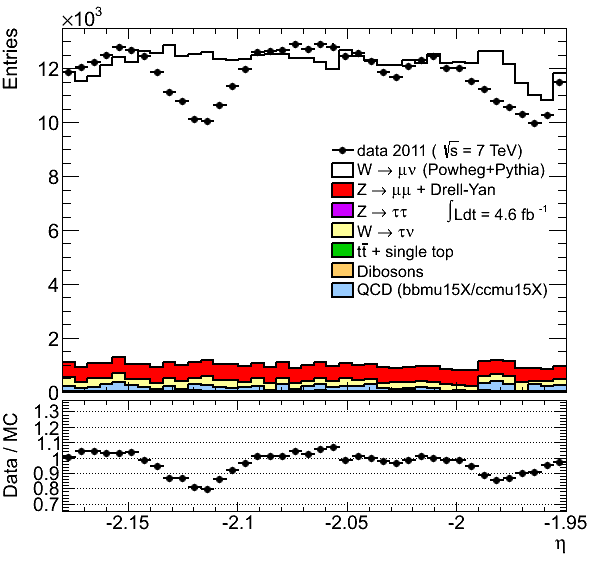
\includegraphics[width=0.66\textwidth]{dates/20130306/figures/both/W_10_C_stack_l_eta_POS} \\
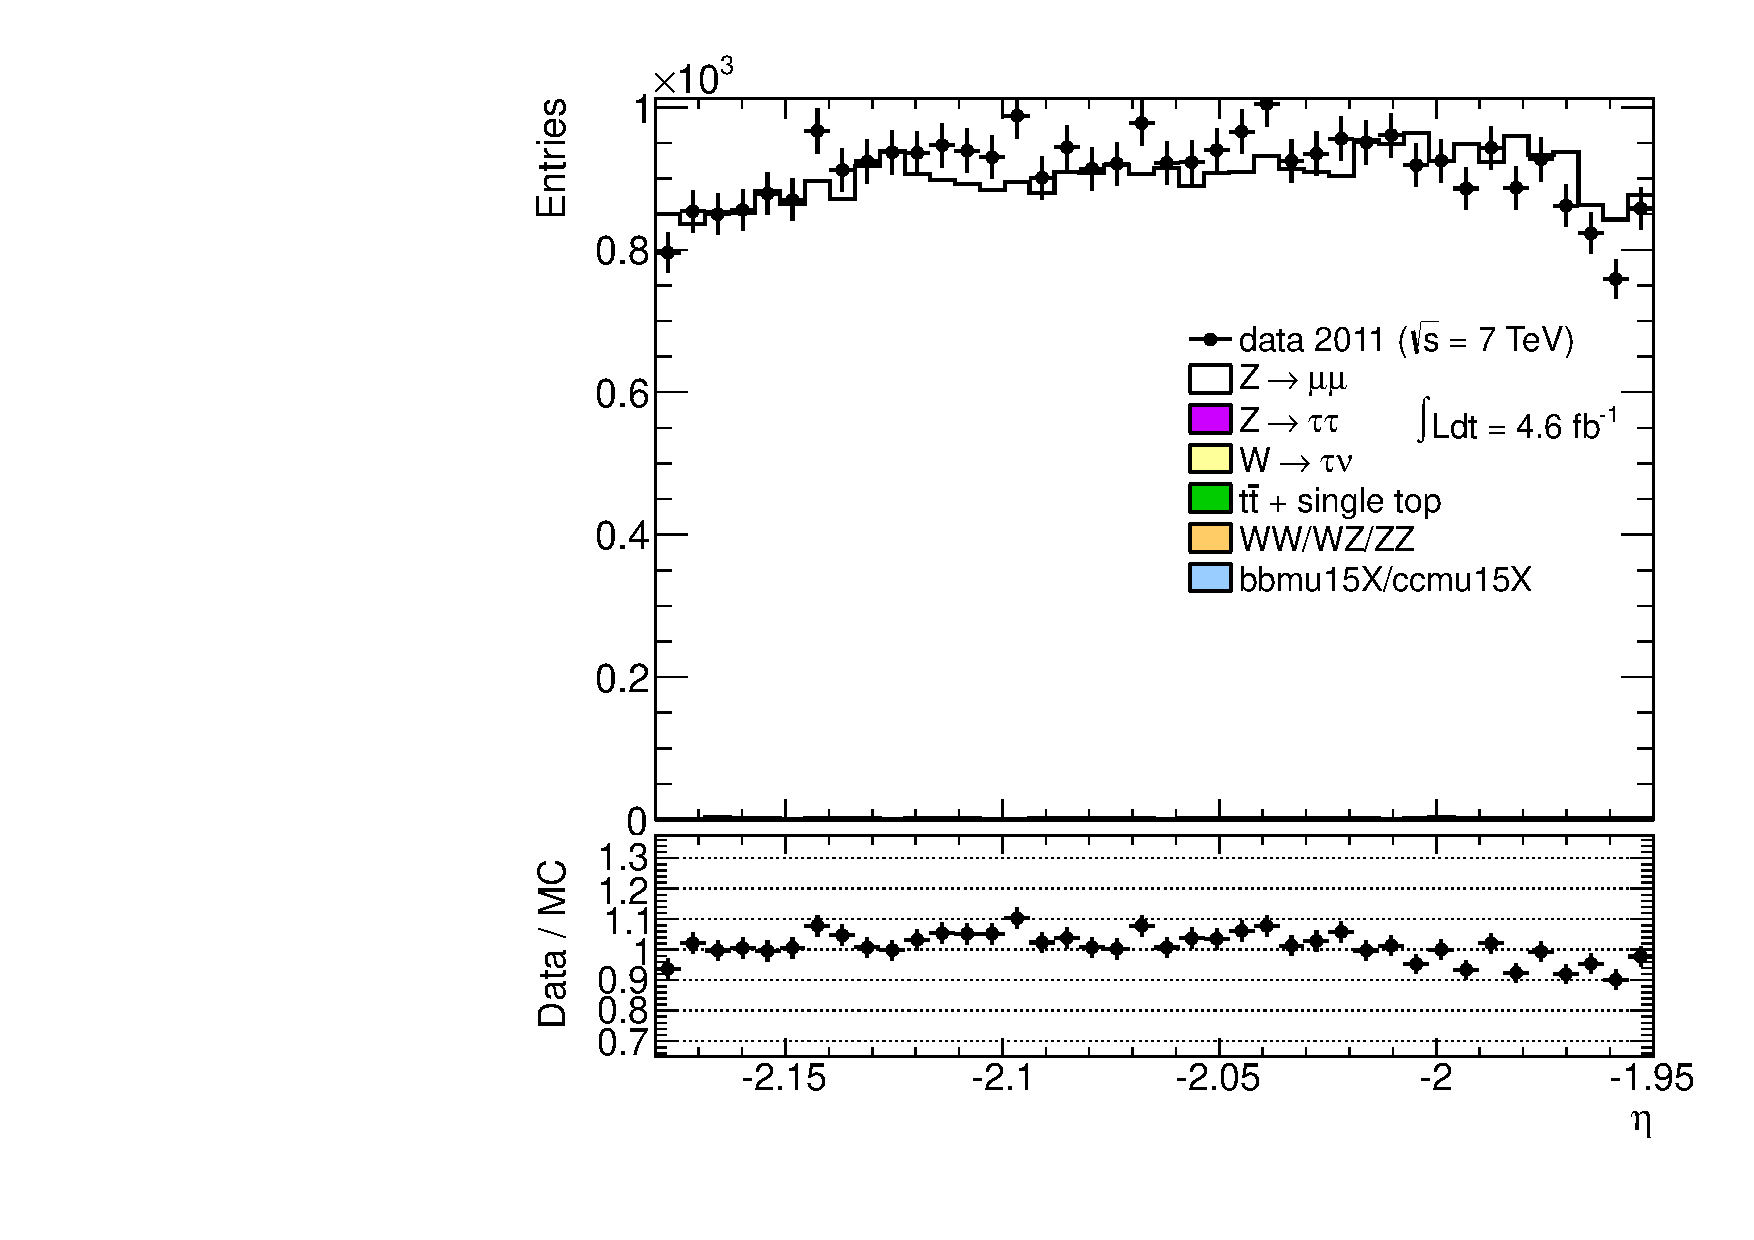
\includegraphics[width=0.66\textwidth]{dates/20130306/figures/both/Z_10_C_stack_lP_eta_ALL.pdf}
\column{.5\textwidth}
A-side $\mu^{+}$ (top: W; bottom: Z)
\centering
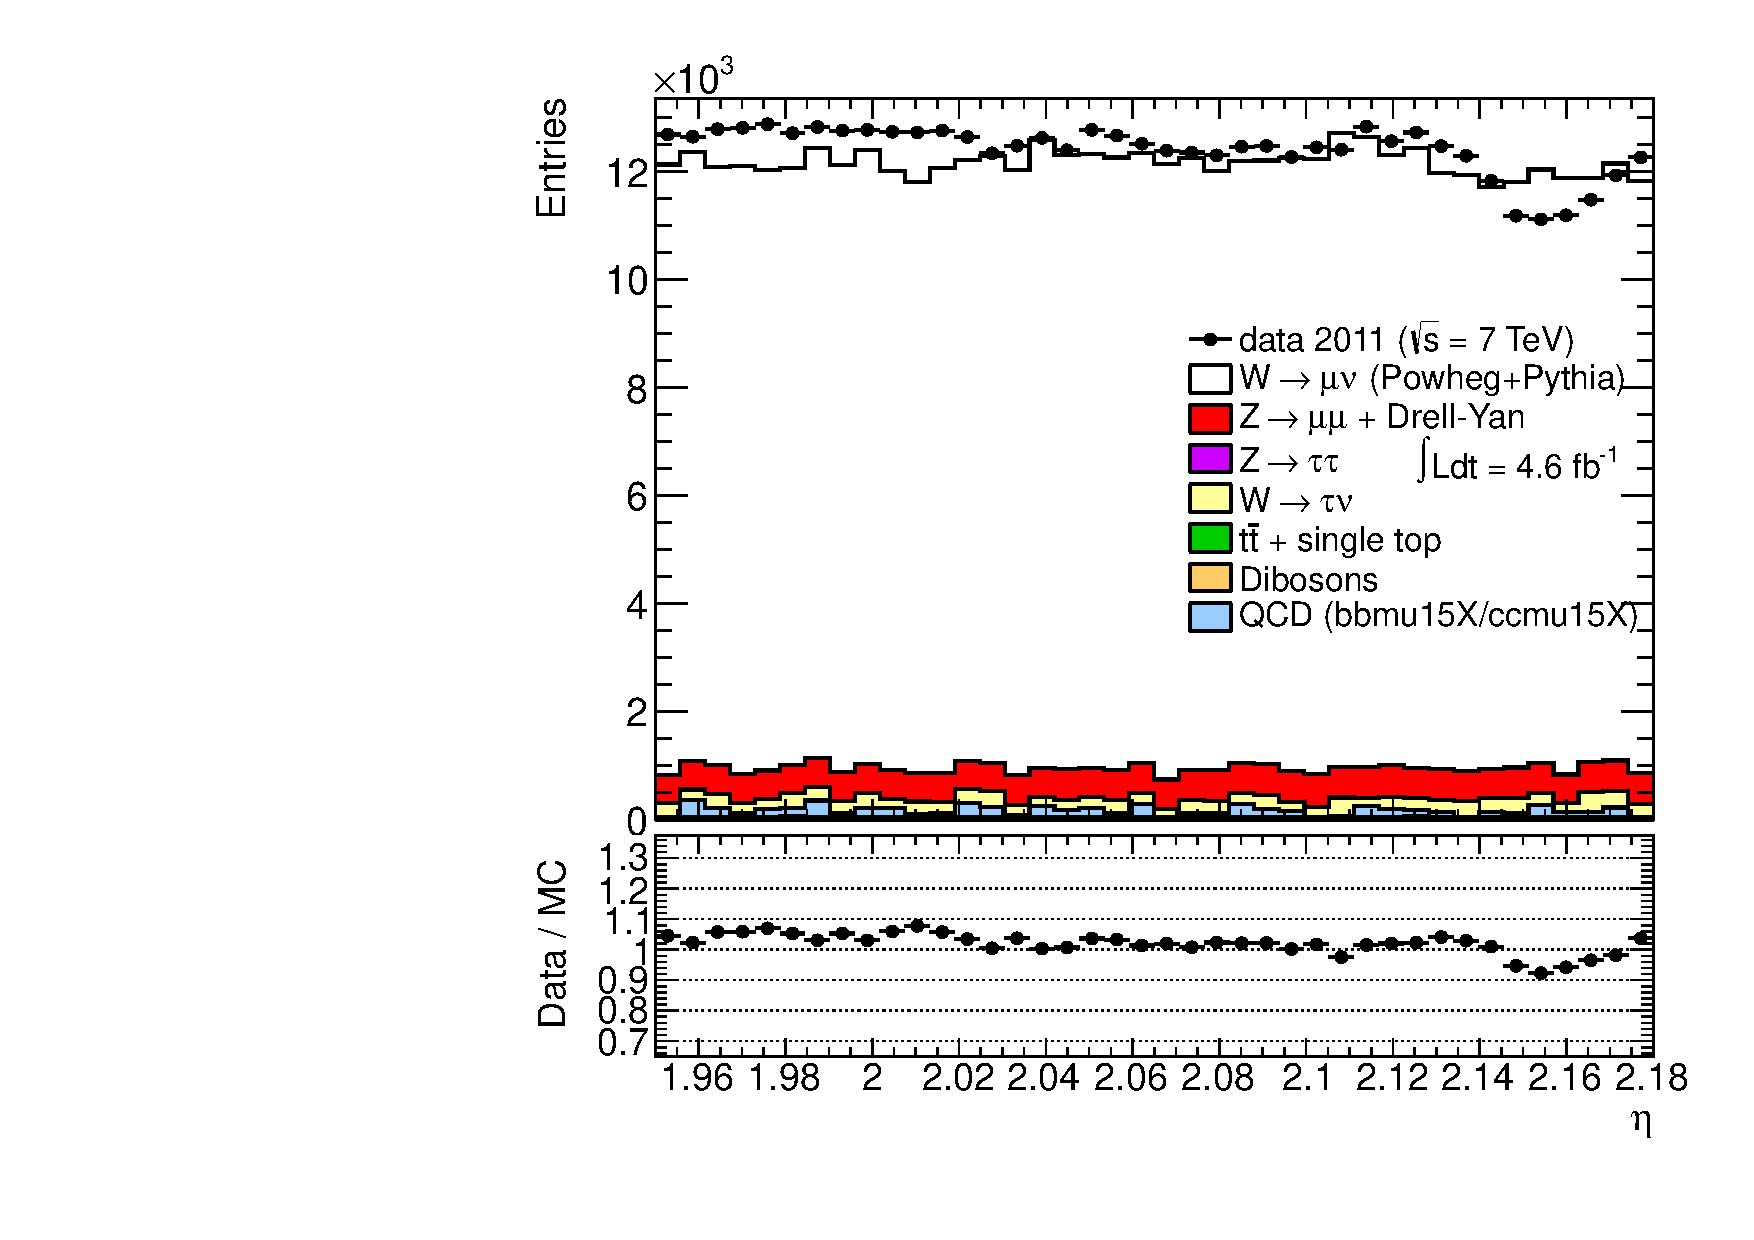
\includegraphics[width=0.66\textwidth]{dates/20130306/figures/both/W_10_A_stack_l_eta_POS} \\
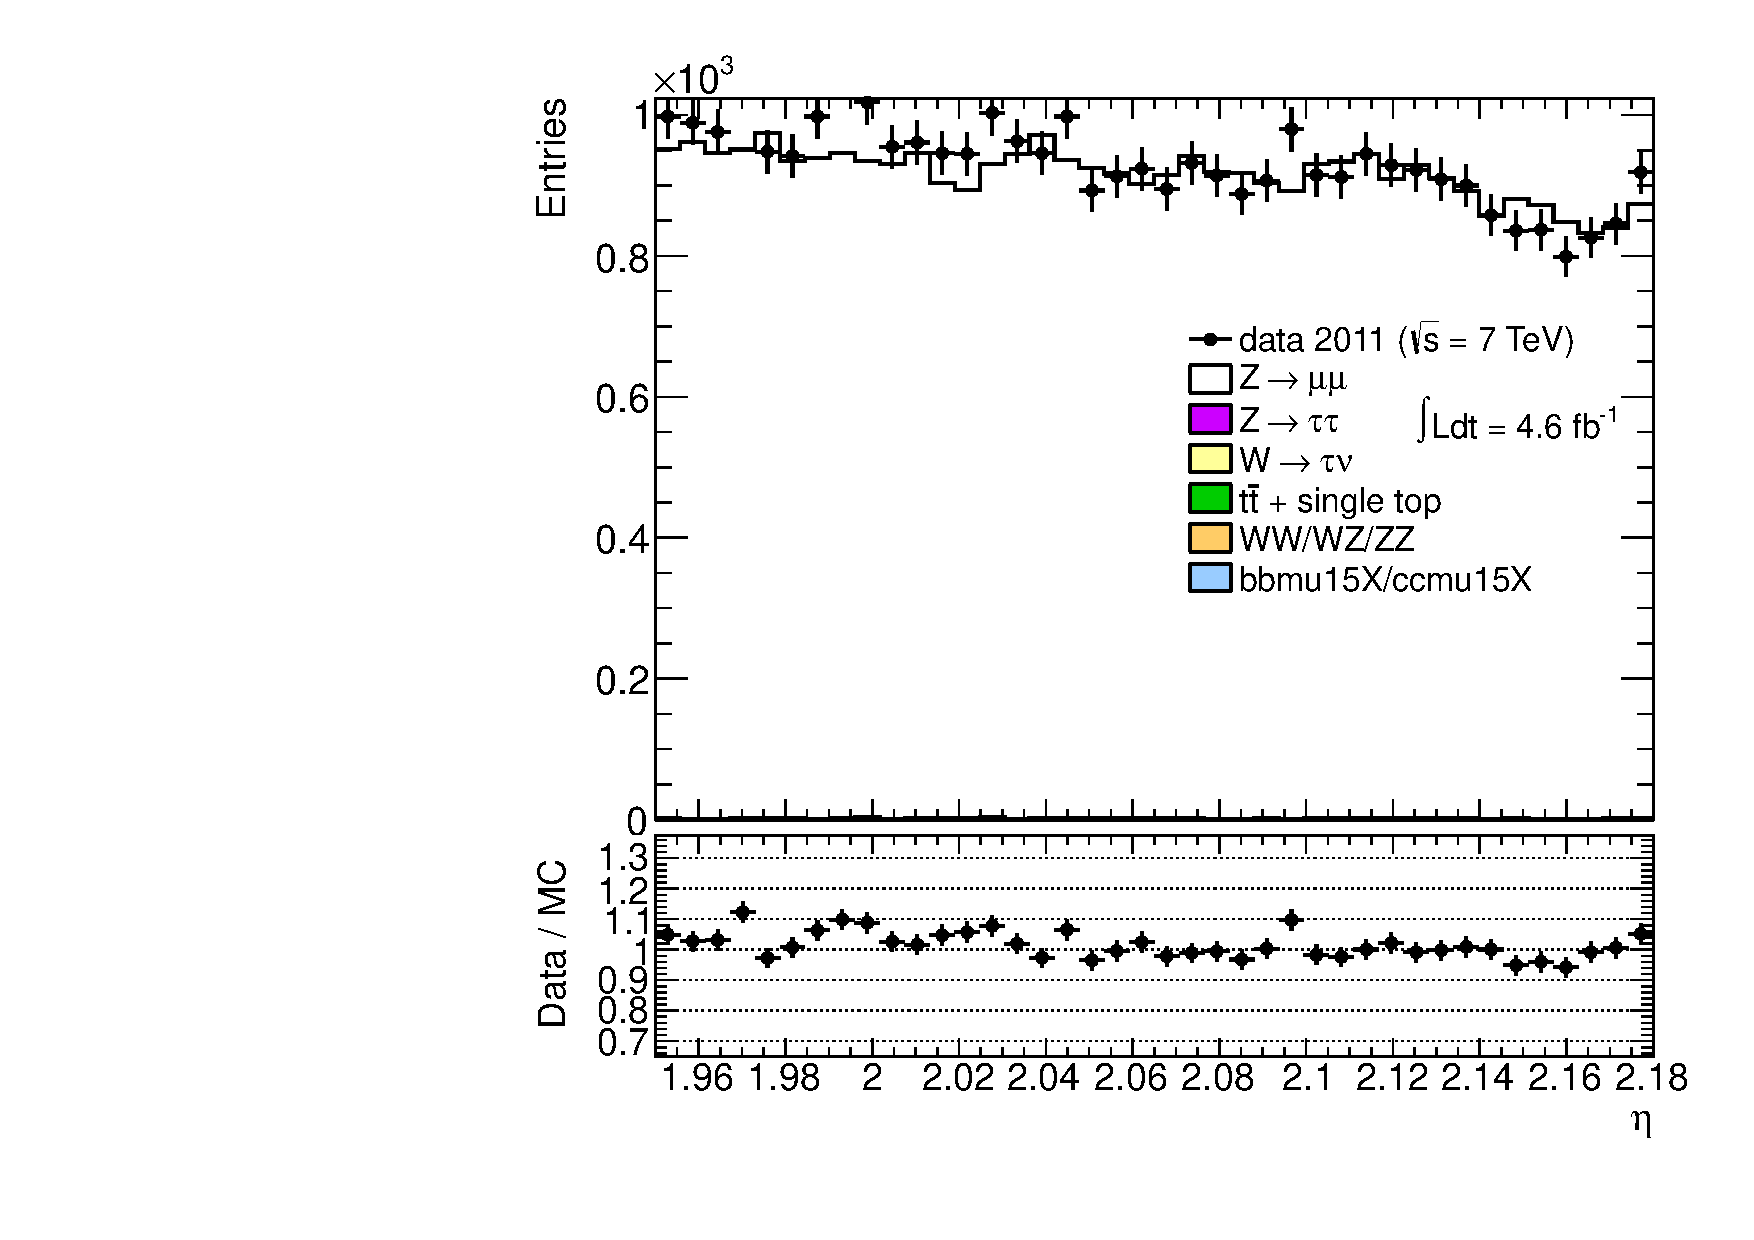
\includegraphics[width=0.66\textwidth]{dates/20130306/figures/both/Z_10_A_stack_lP_eta_ALL.pdf} 
\cole
}
\slide{ $\mu^{-}$: bin 10 ($1.95<\eta<2.18$) } {
\colb[T]
\column{.5\textwidth}
C-side $\mu^{-}$ (top: W; bottom: Z)
\centering
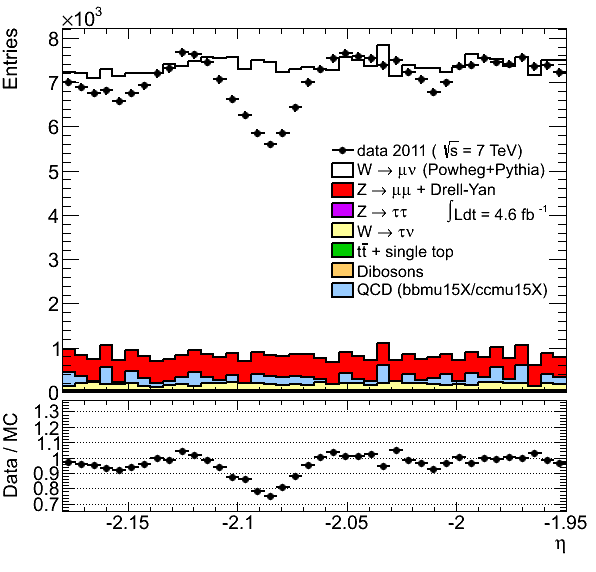
\includegraphics[width=0.66\textwidth]{dates/20130306/figures/both/W_10_C_stack_l_eta_NEG} \\
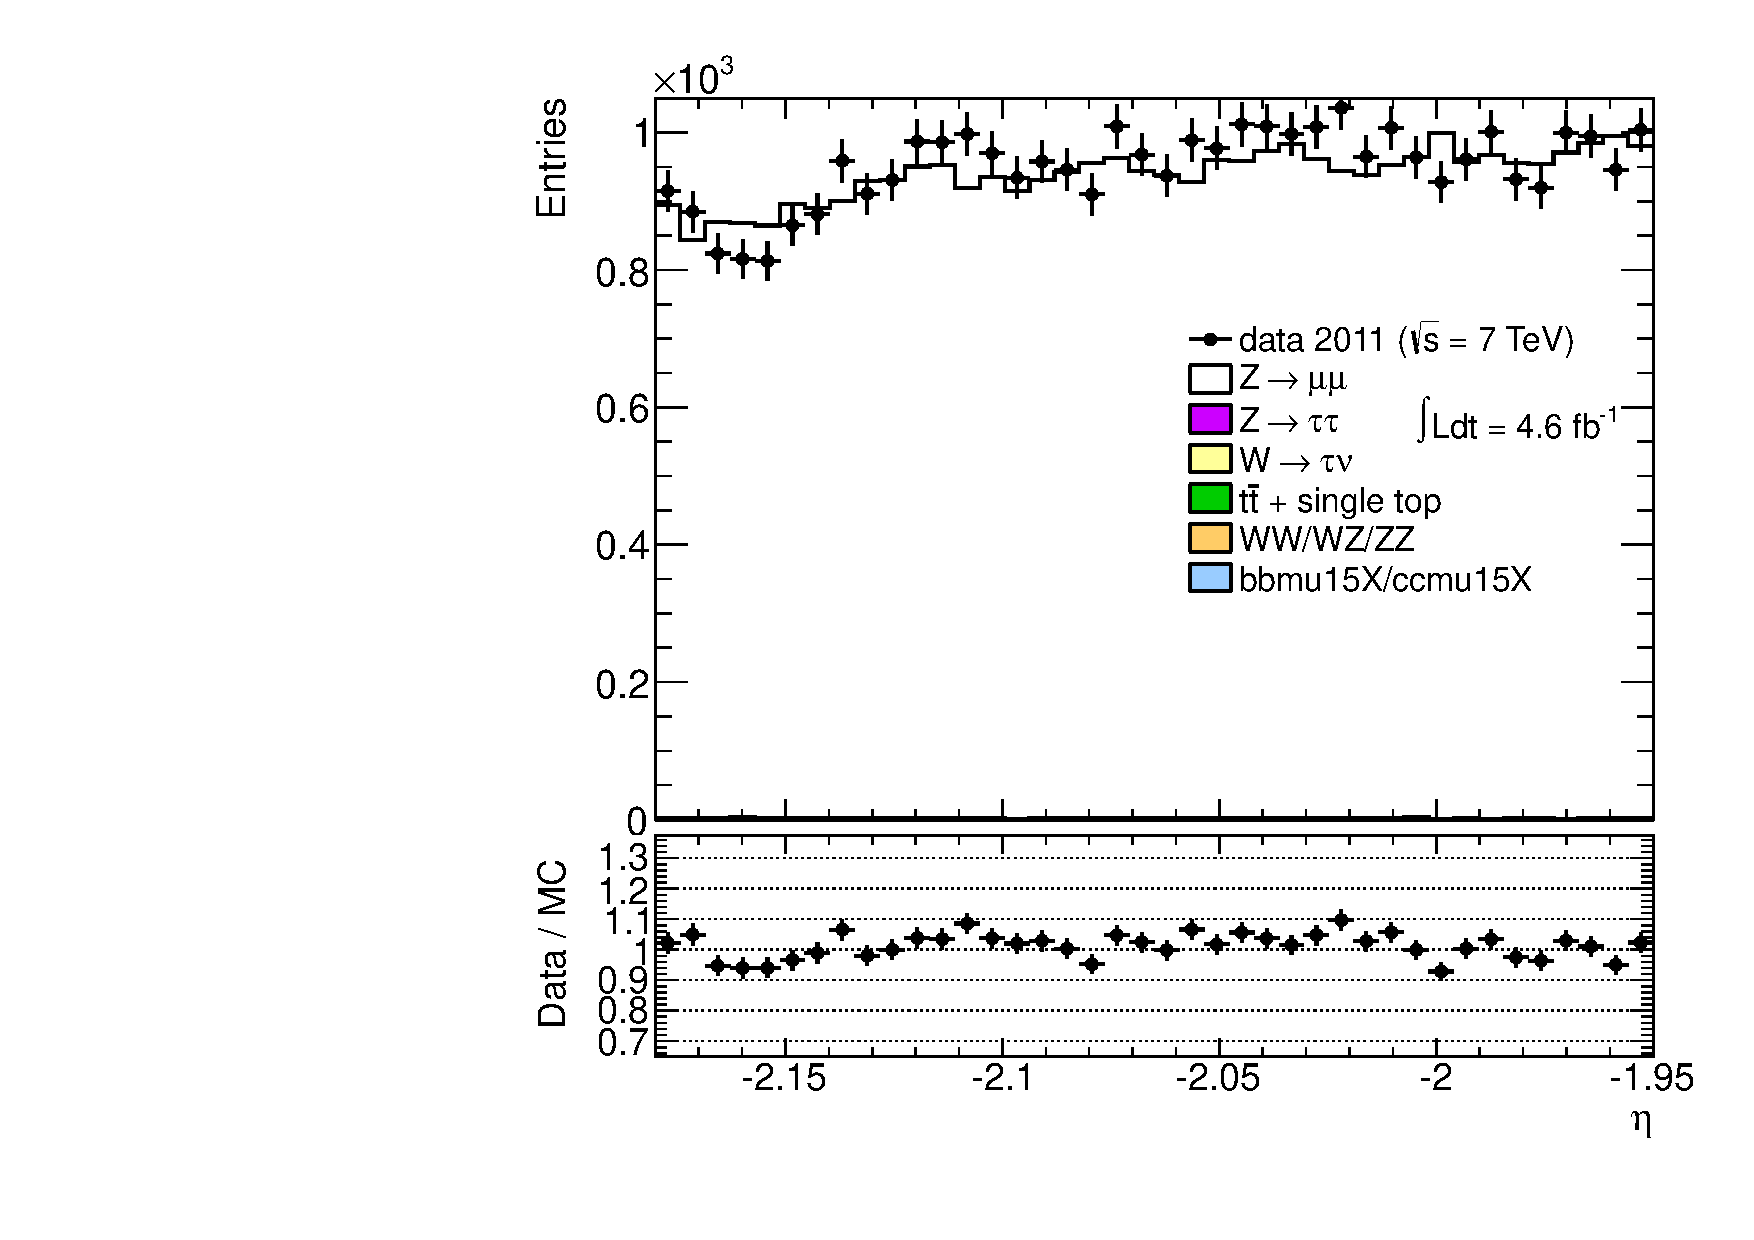
\includegraphics[width=0.66\textwidth]{dates/20130306/figures/both/Z_10_C_stack_lN_eta_ALL.pdf}
\column{.5\textwidth}
A-side $\mu^{-}$ (top: W; bottom: Z)
\centering
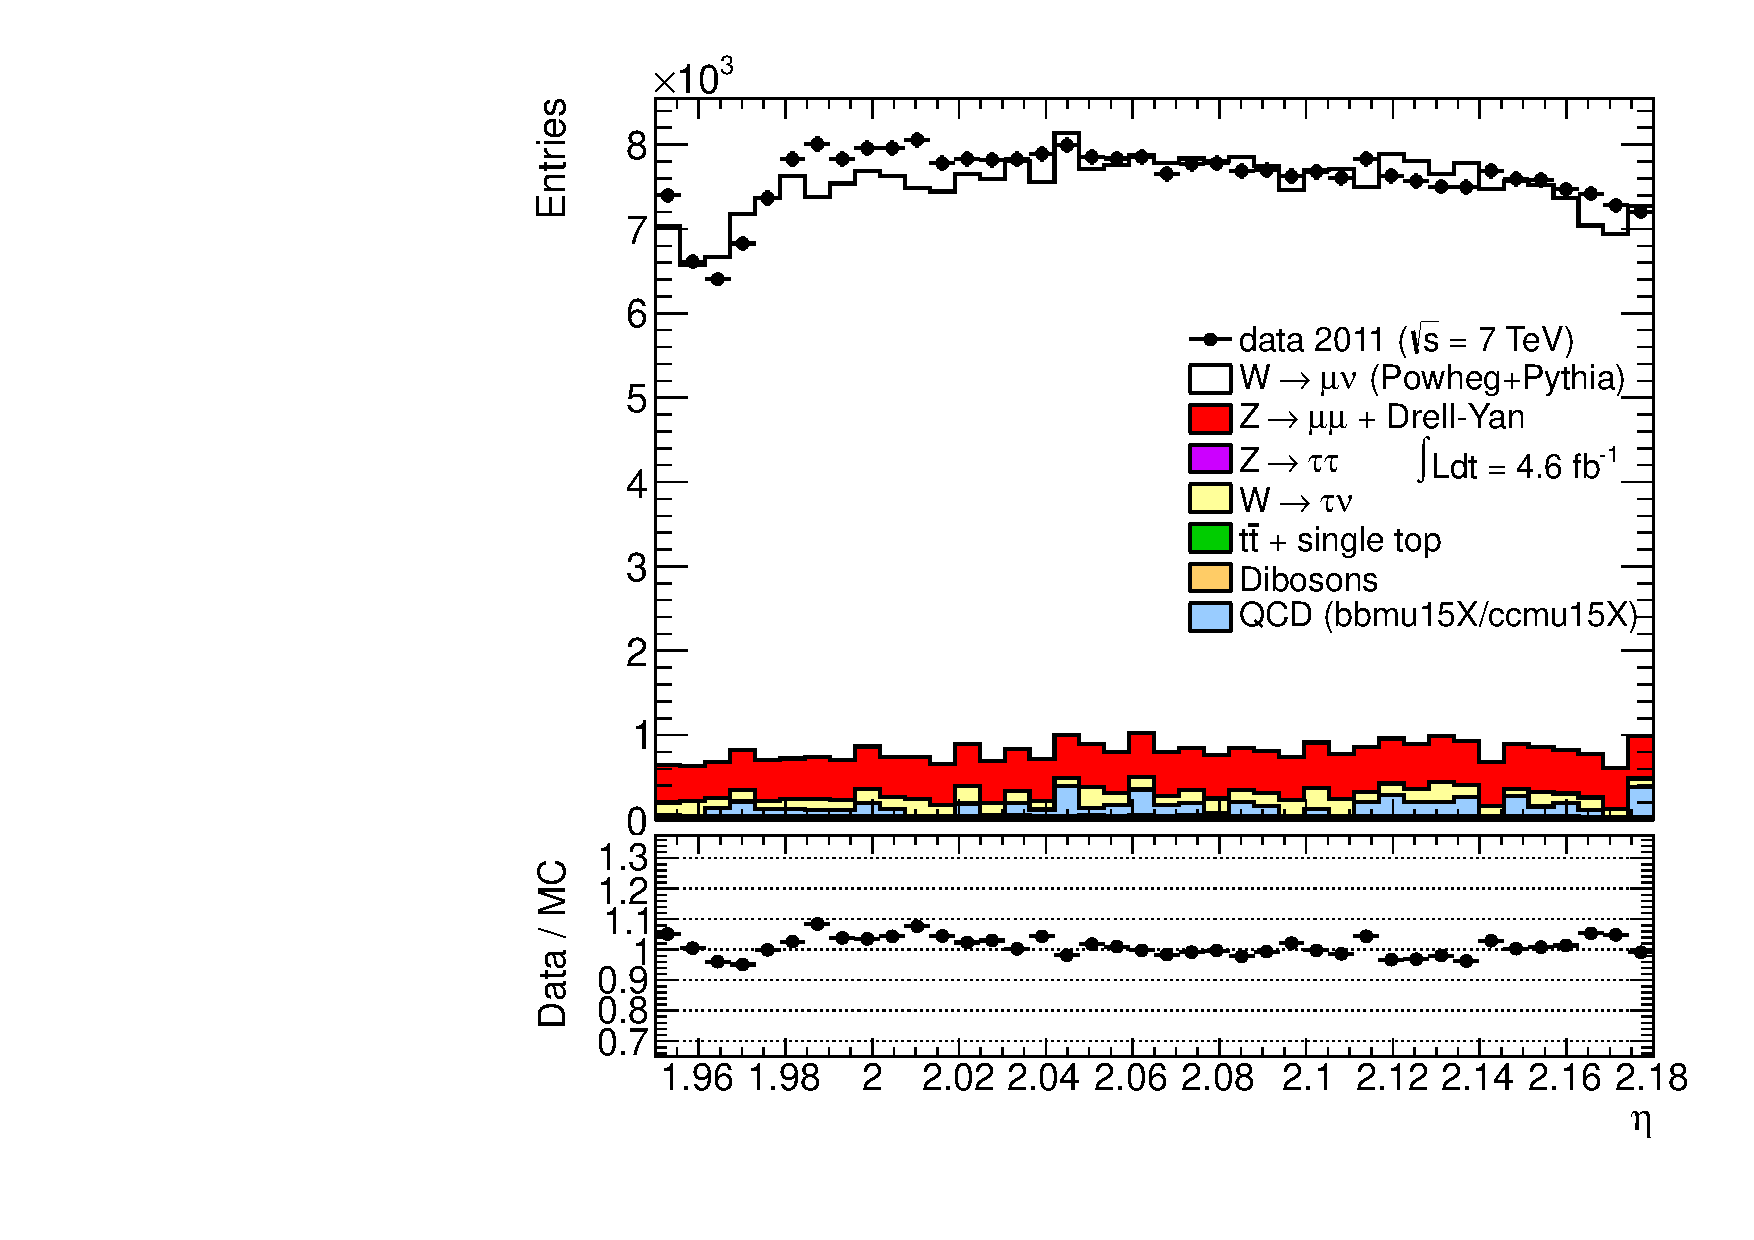
\includegraphics[width=0.66\textwidth]{dates/20130306/figures/both/W_10_A_stack_l_eta_NEG} \\
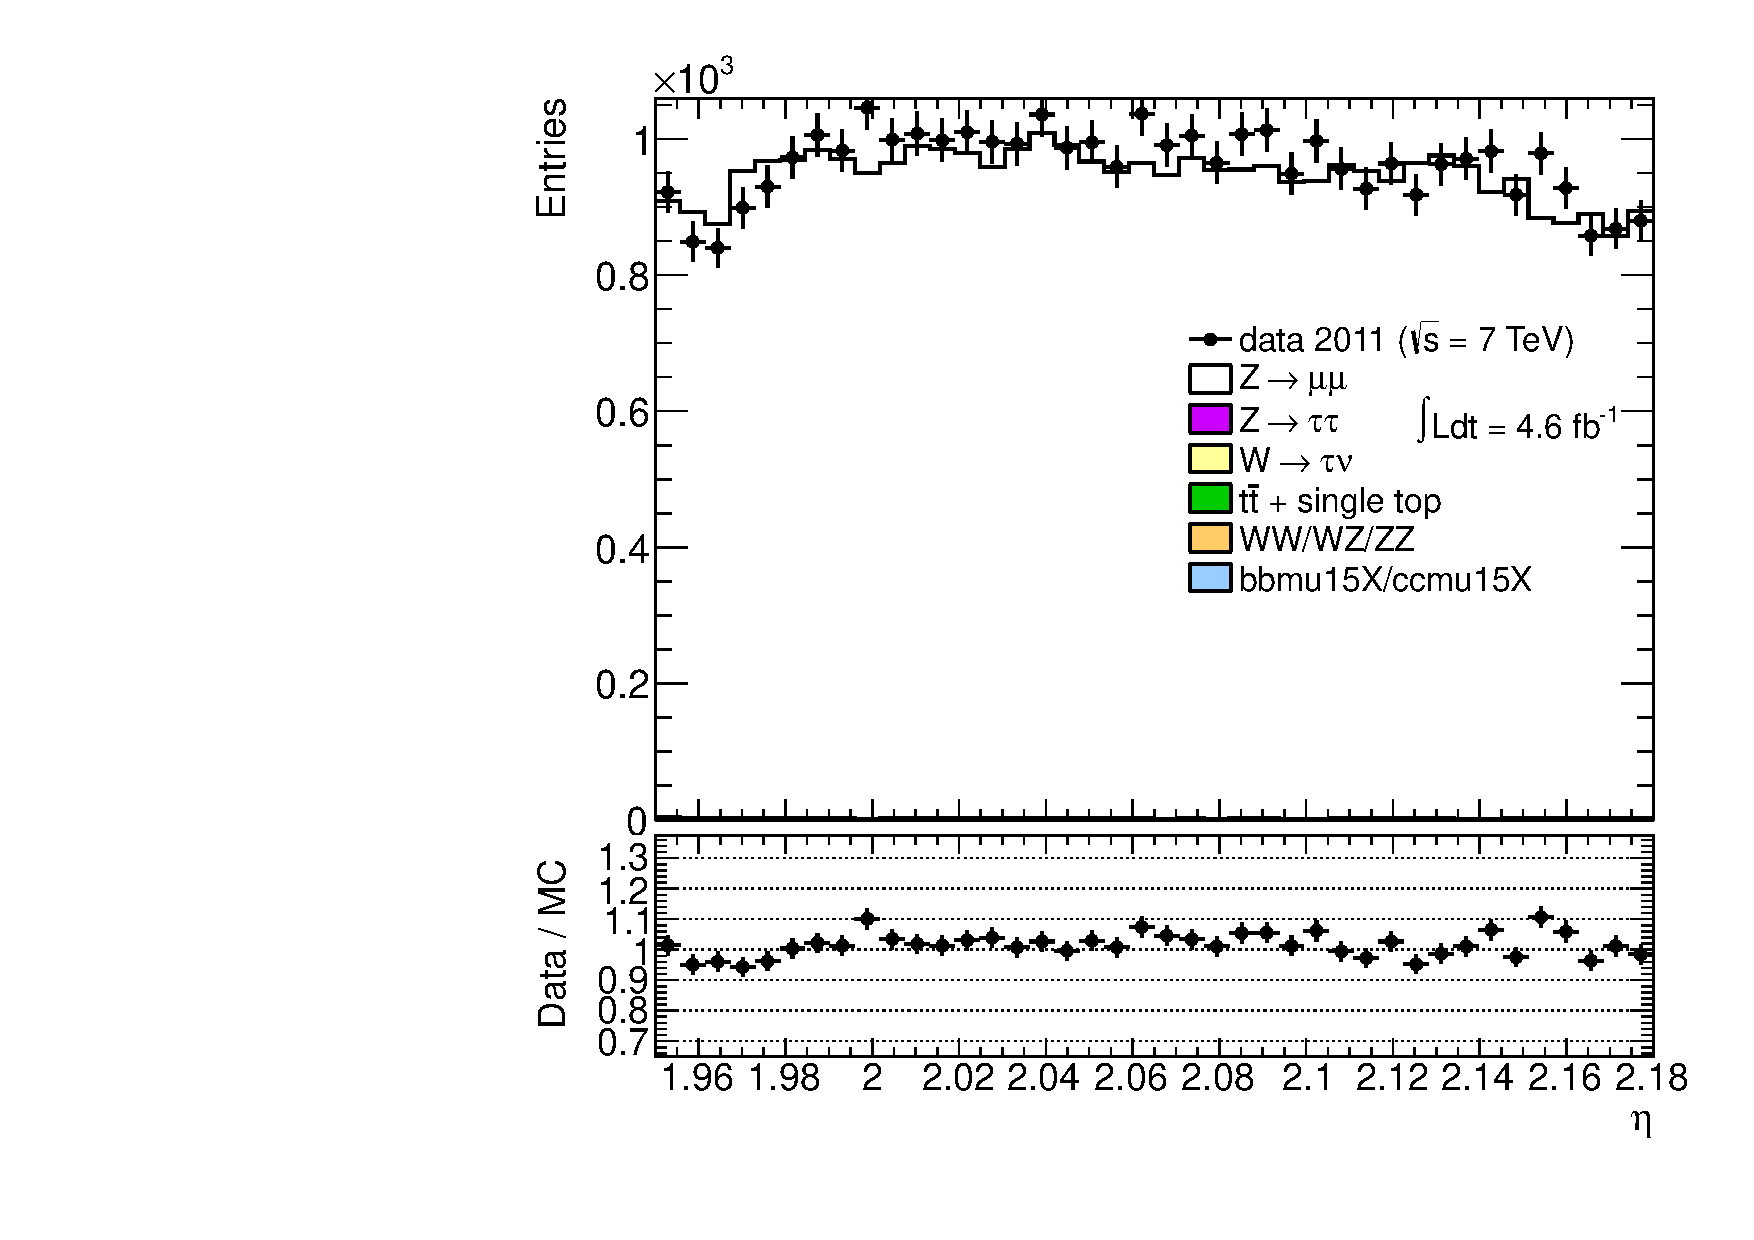
\includegraphics[width=0.66\textwidth]{dates/20130306/figures/both/Z_10_A_stack_lN_eta_ALL.pdf} 
\cole
}

\slide{ Z bin 10 $\mu^{+}$: nominal (for reference) } {
   Perhaps trigger matching is not doing the right thing in Zs? \\
   We can implicitly require the probe muon to have fired the trigger \\
   by asking the \red{tag} muon to fail it.
}
\slide{ Z bin 10 $\mu^{+}$: nominal (for reference) } {
\colb[T]
\column{.5\textwidth}
C-side $\mu^{-}$ (top: W; bottom: Z)
\centering
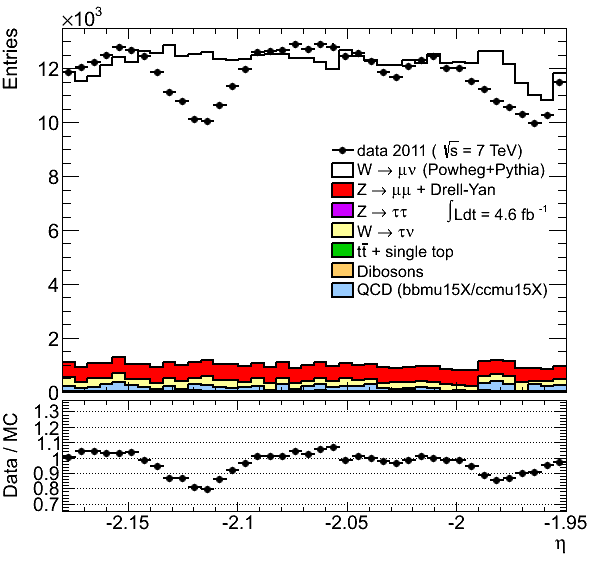
\includegraphics[width=0.66\textwidth]{dates/20130306/figures/both/W_10_C_stack_l_eta_POS} \\
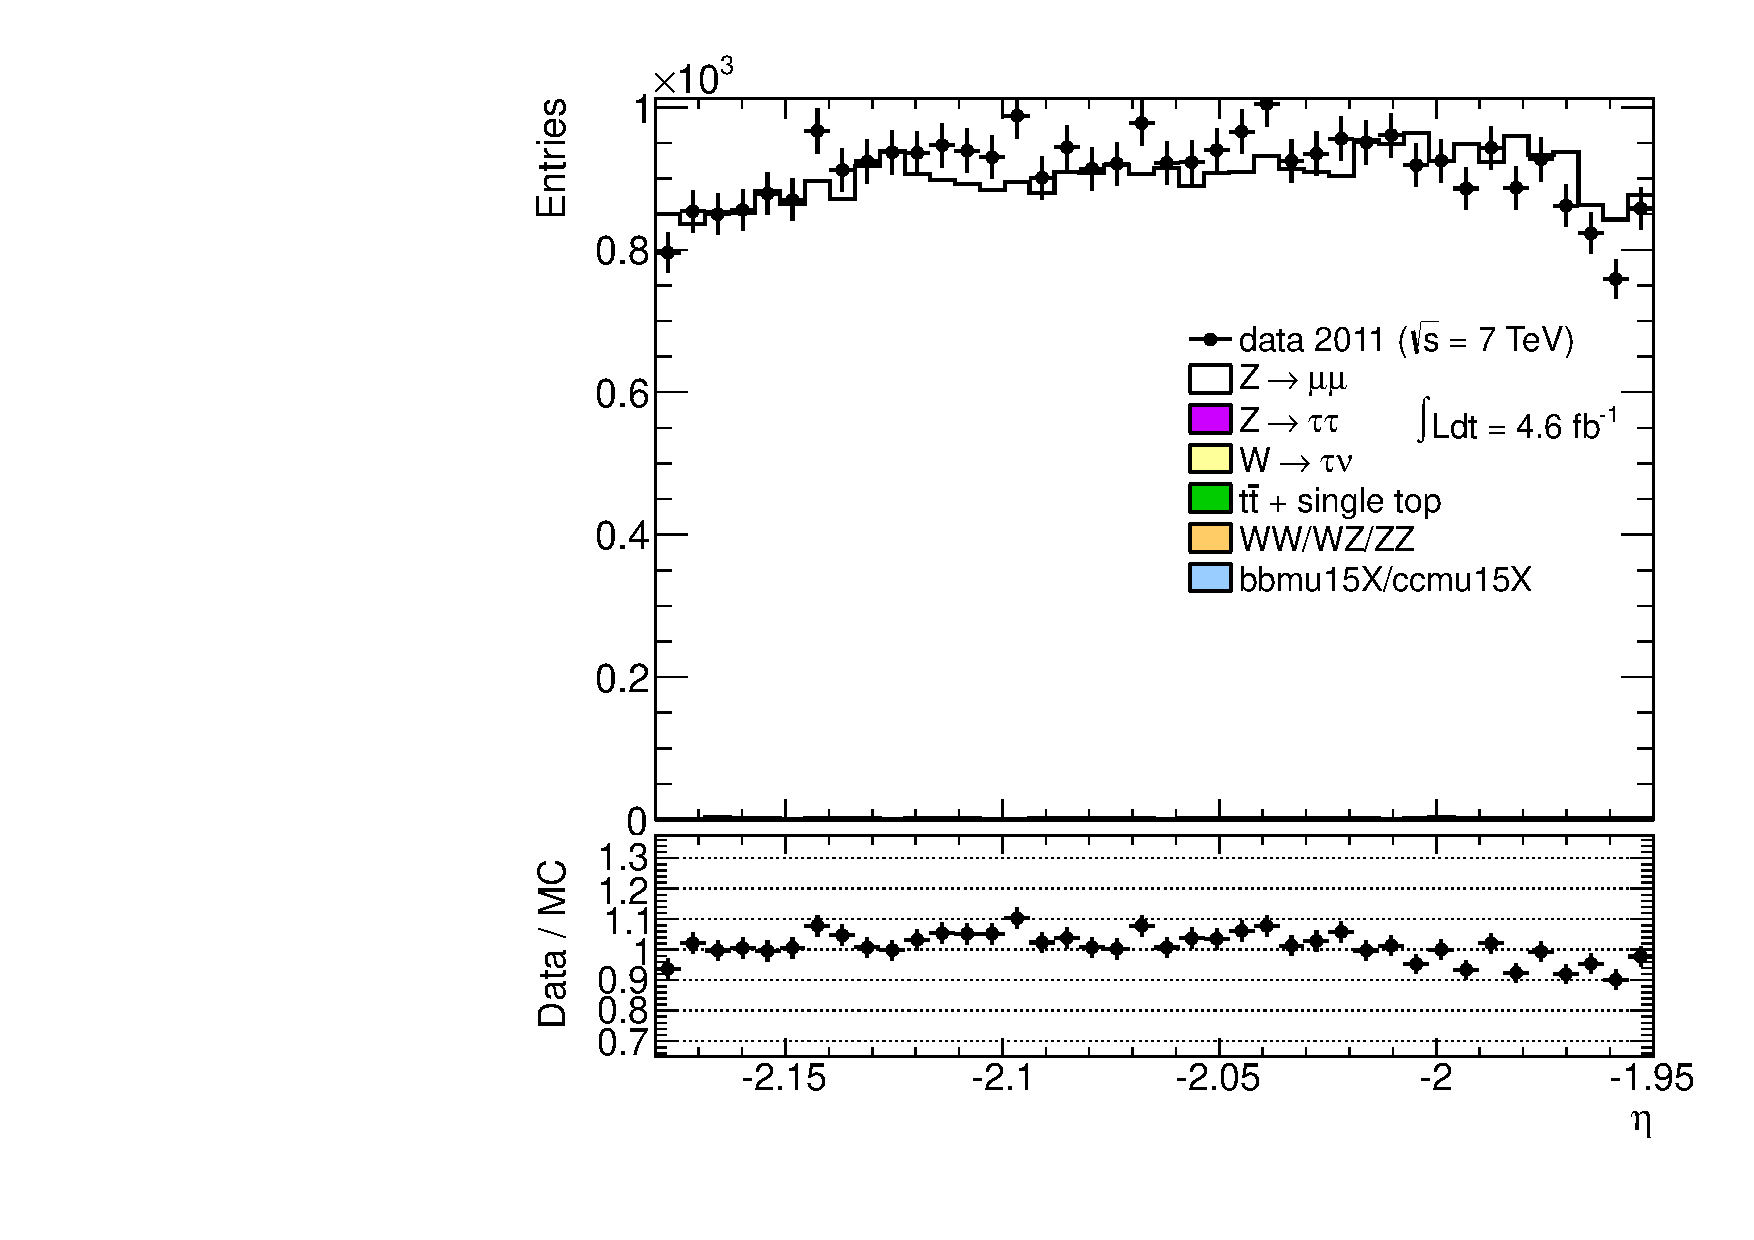
\includegraphics[width=0.66\textwidth]{dates/20130306/figures/both/Z_10_C_stack_lP_eta_ALL.pdf}
\column{.5\textwidth}
A-side $\mu^{-}$ (top: W; bottom: Z)
\centering
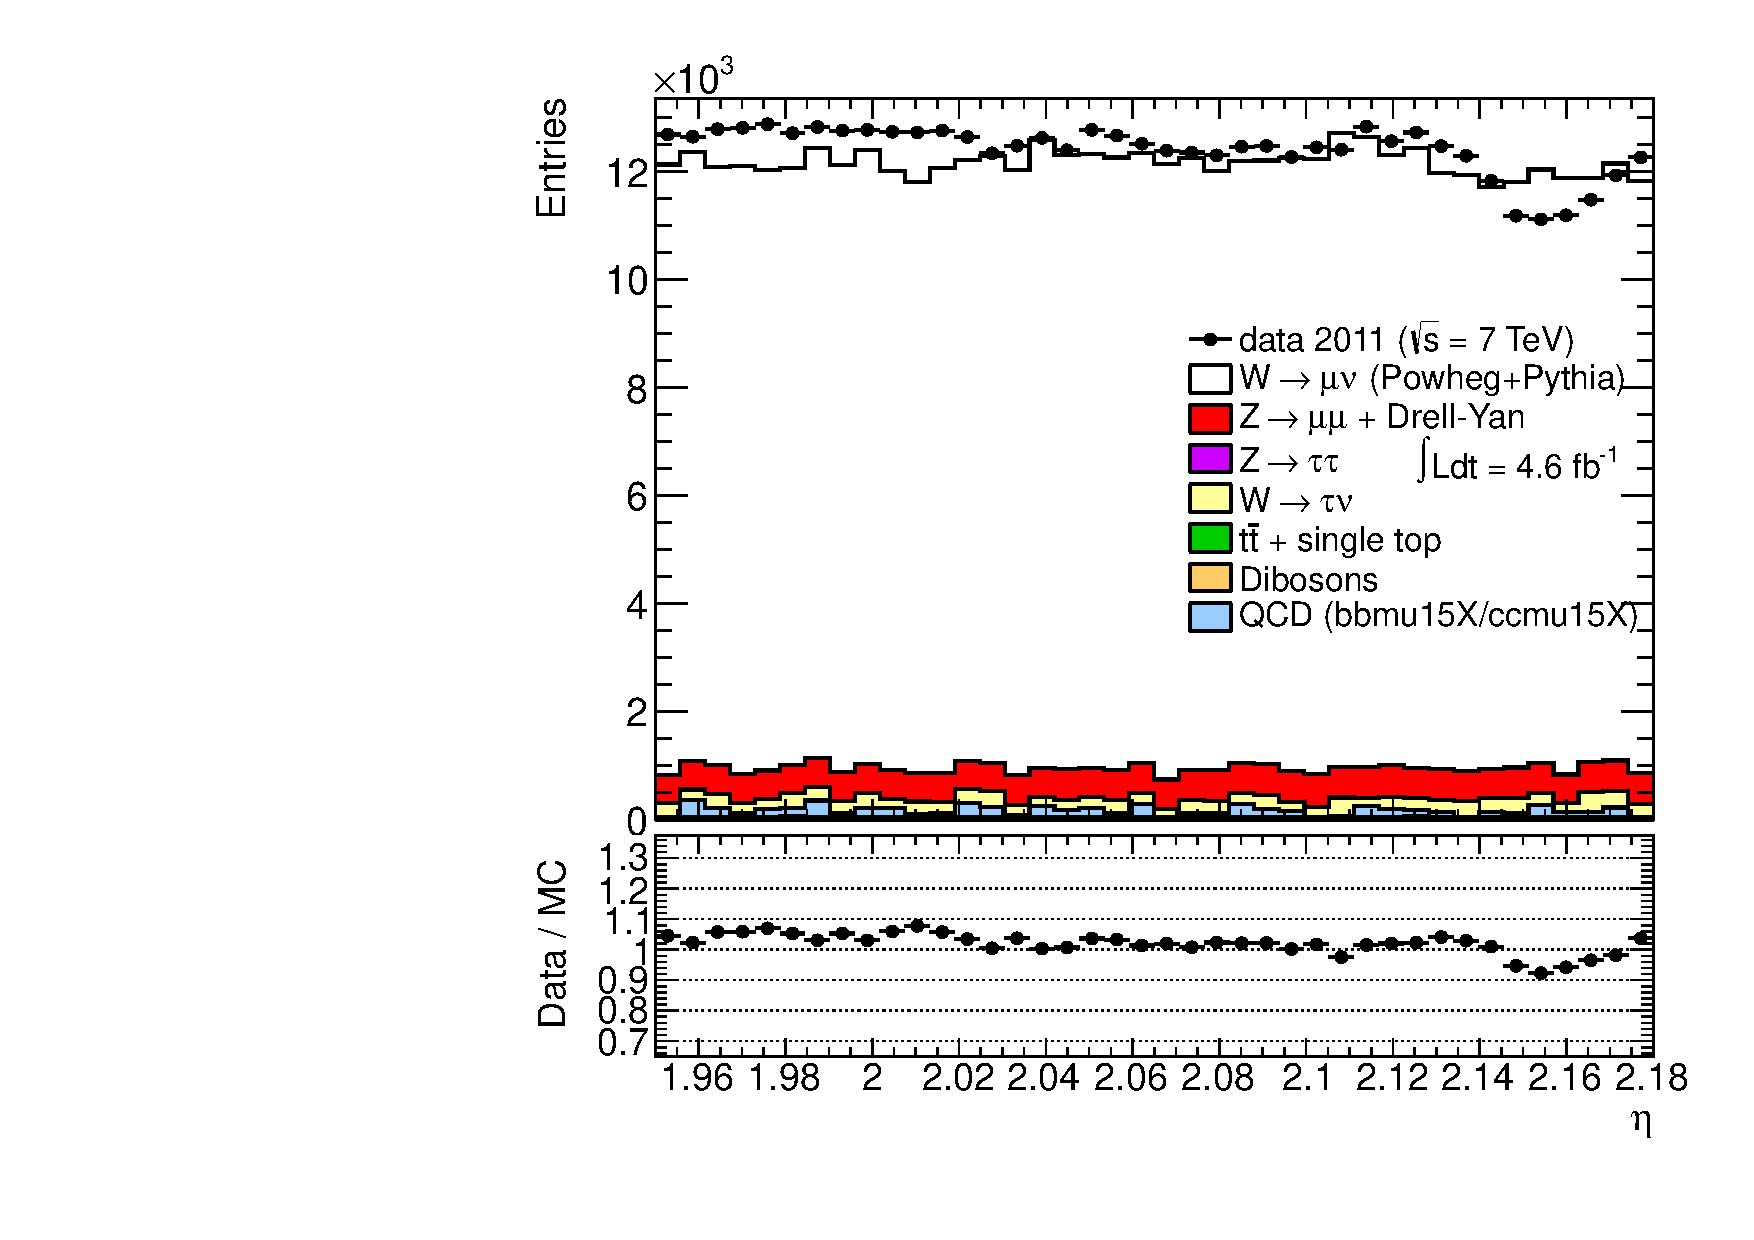
\includegraphics[width=0.66\textwidth]{dates/20130306/figures/both/W_10_A_stack_l_eta_POS} \\
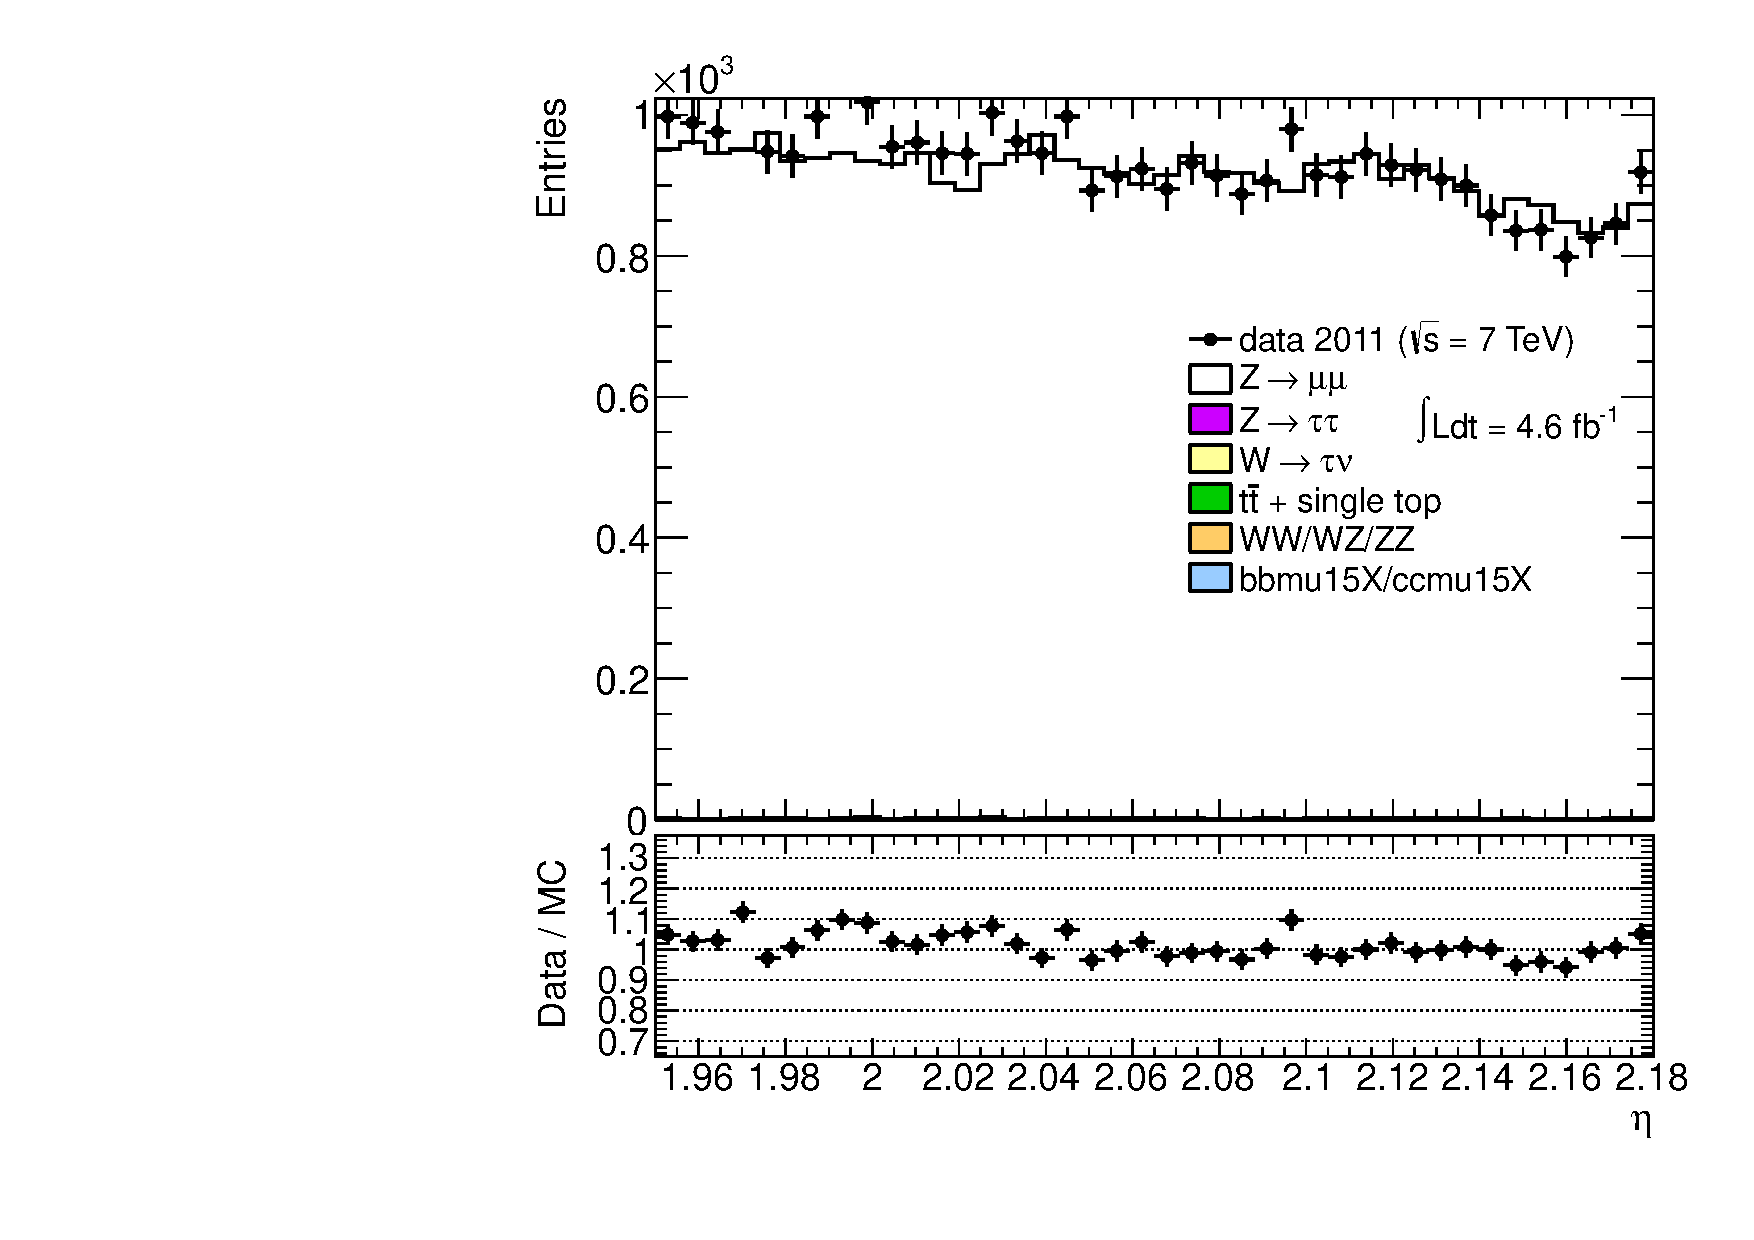
\includegraphics[width=0.66\textwidth]{dates/20130306/figures/both/Z_10_A_stack_lP_eta_ALL.pdf} 
\cole
}
\slide{ Z bin 10 $\mu^{+}$: require tag muon to \red{fail} trigger } {
\colb[T]
\column{.5\textwidth}
C-side $\mu^{-}$ (top: W; bottom: Z)
\centering
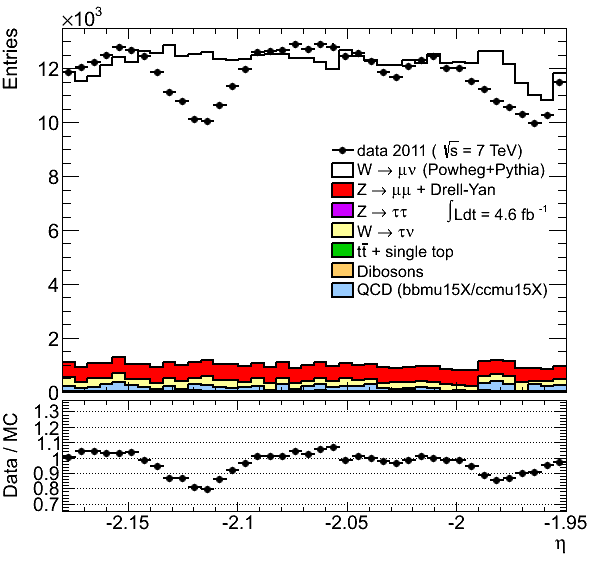
\includegraphics[width=0.66\textwidth]{dates/20130306/figures/both/W_10_C_stack_l_eta_POS} \\
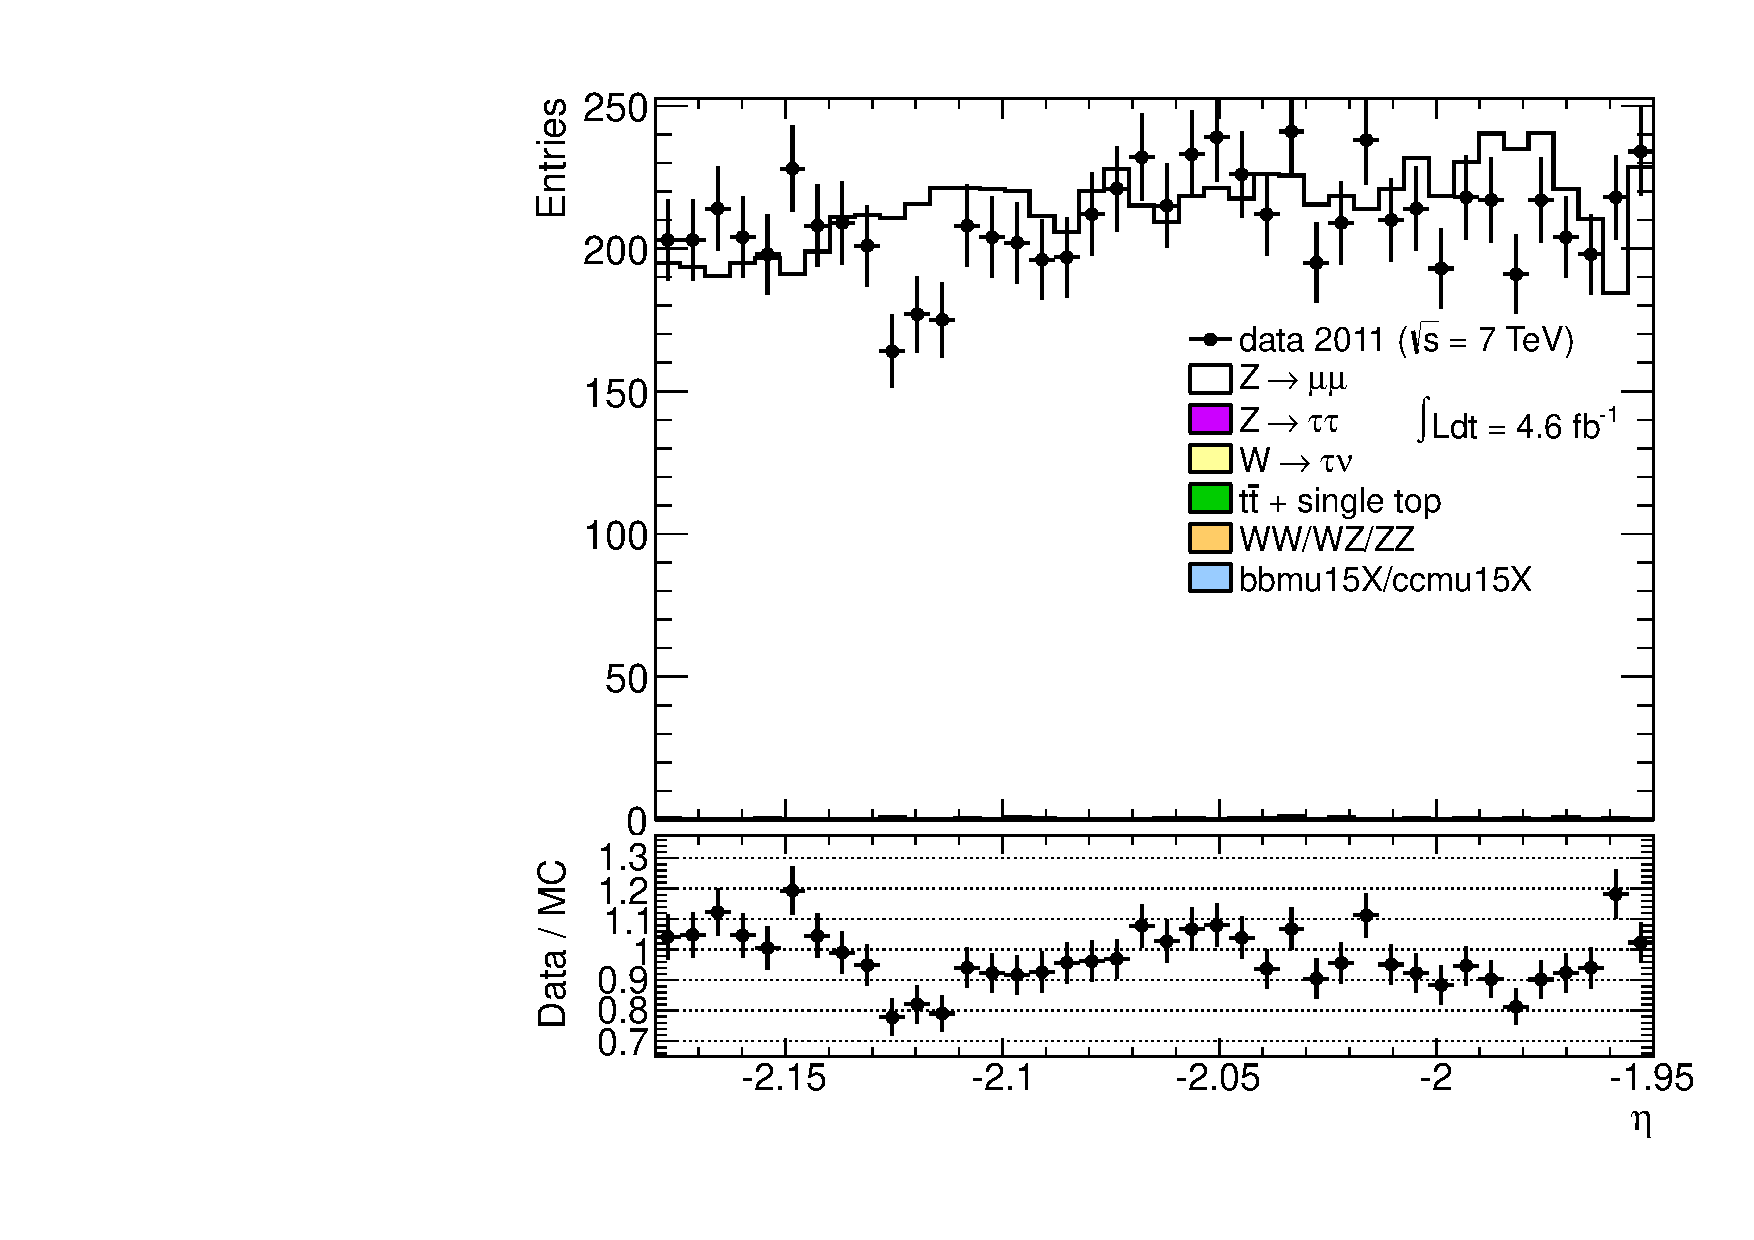
\includegraphics[width=0.66\textwidth]{dates/20130306/figures/both/Ztinv_10_C_stack_lP_eta_ALL.pdf}
\column{.5\textwidth}
A-side $\mu^{-}$ (top: W; bottom: Z)
\centering
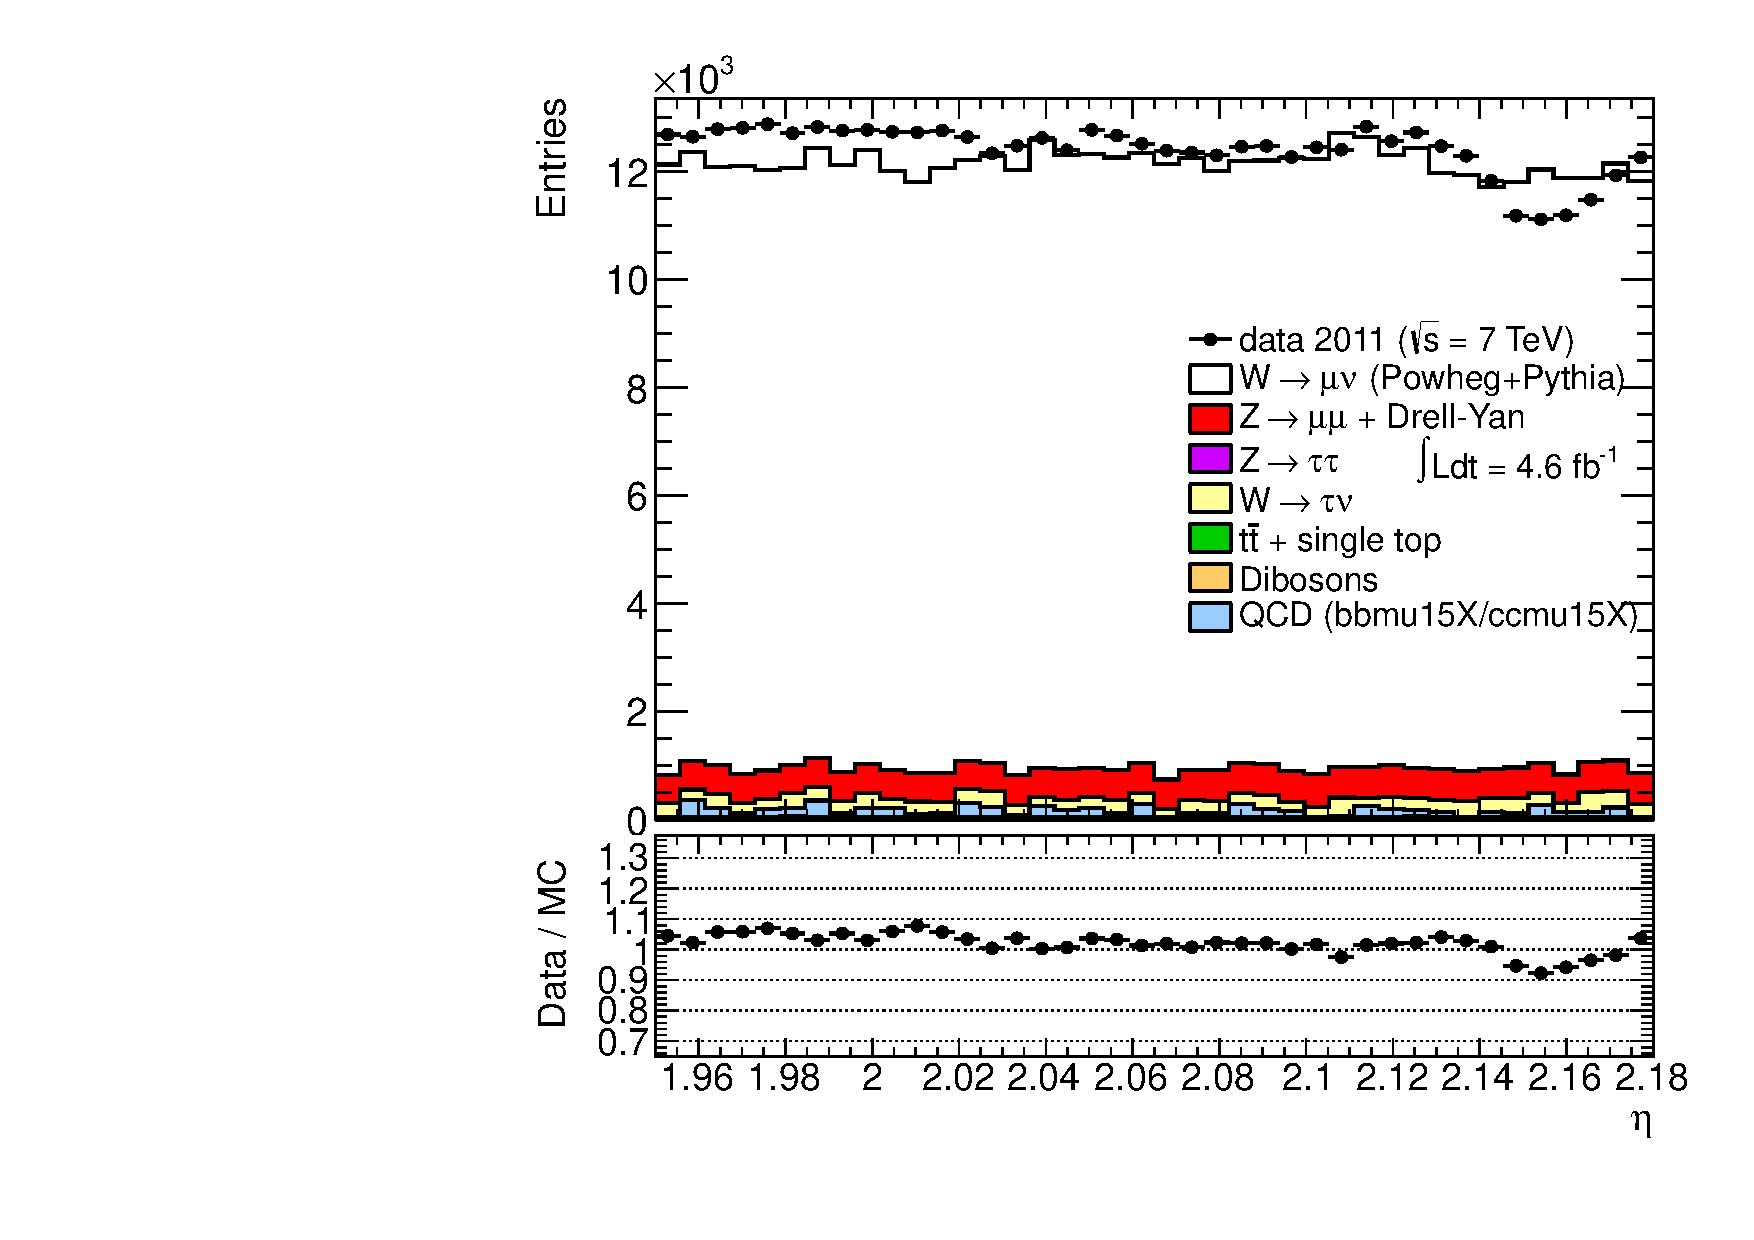
\includegraphics[width=0.66\textwidth]{dates/20130306/figures/both/W_10_A_stack_l_eta_POS} \\
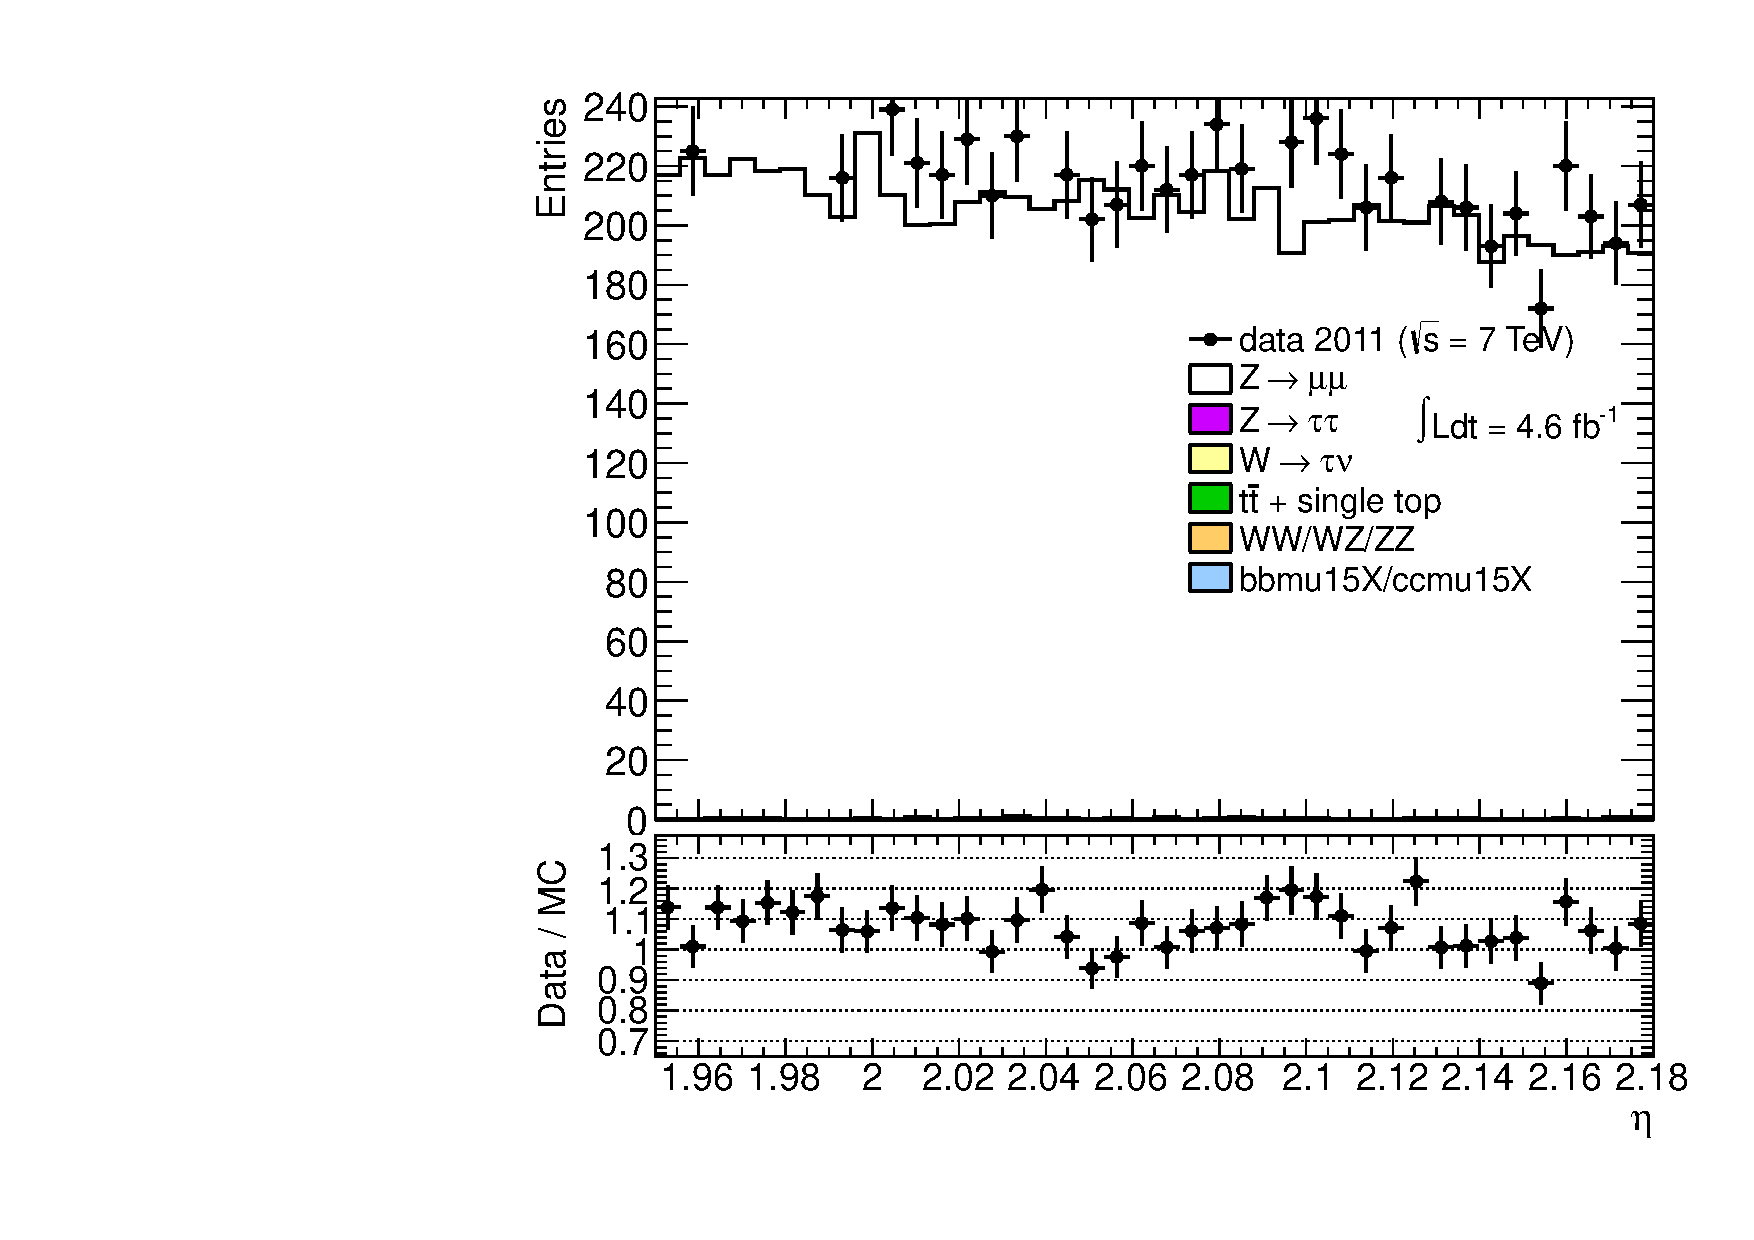
\includegraphics[width=0.66\textwidth]{dates/20130306/figures/both/Ztinv_10_A_stack_lP_eta_ALL.pdf} 
\cole
}
\slide{ Z: require tag muon to \red{fail} trigger } {
Interpretation:
\iteb
\item If we require that both Z muons match trigger: \red{no dip}
\item If we require that probe muon matches trigger (tag may or may not): \red{no dip}
\item If we require that tag fails trigger (so probe must fire!), we \red{see W-like dip}
\item This is especially true in the 10th \eta\ bin (but not so much in the 8th bin)
\iteb
\item Somehow, requiring the probe muon to match to an EF trigger for muons around the dip \red{at the AOD or D3PD level} does not actually imply that this muon triggered in hardware?
\itee
\itee
}

% period, bin 10, -
\slide{ $\mu^{-}$: bin 10 ($1.95<\eta<2.18$), period dependence } {
Let's examine period dependence of the dip in W. \\
\small{ note: Z plots are always full-2011 in plots below }
}
\slide{ $\mu^{-}$: bin 10 ($1.95<\eta<2.18$), all 2011 } {
\colb[T]
\column{.5\textwidth}
C-side (top: W; bottom: Z)
\centering
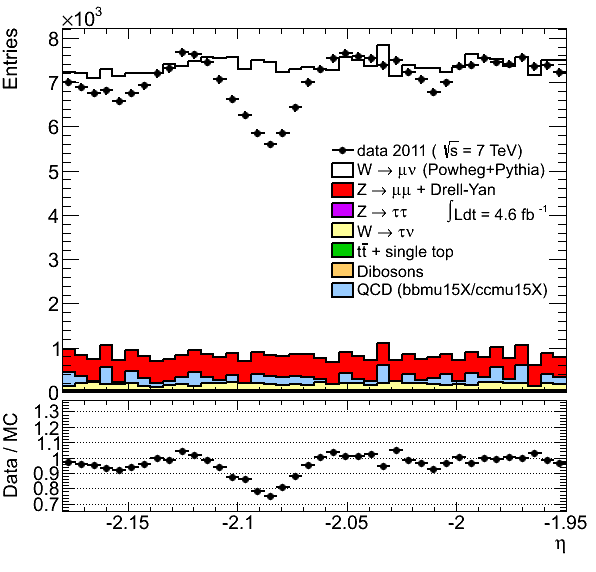
\includegraphics[width=0.66\textwidth]{dates/20130306/figures/both/W_10_C_stack_l_eta_NEG} \\
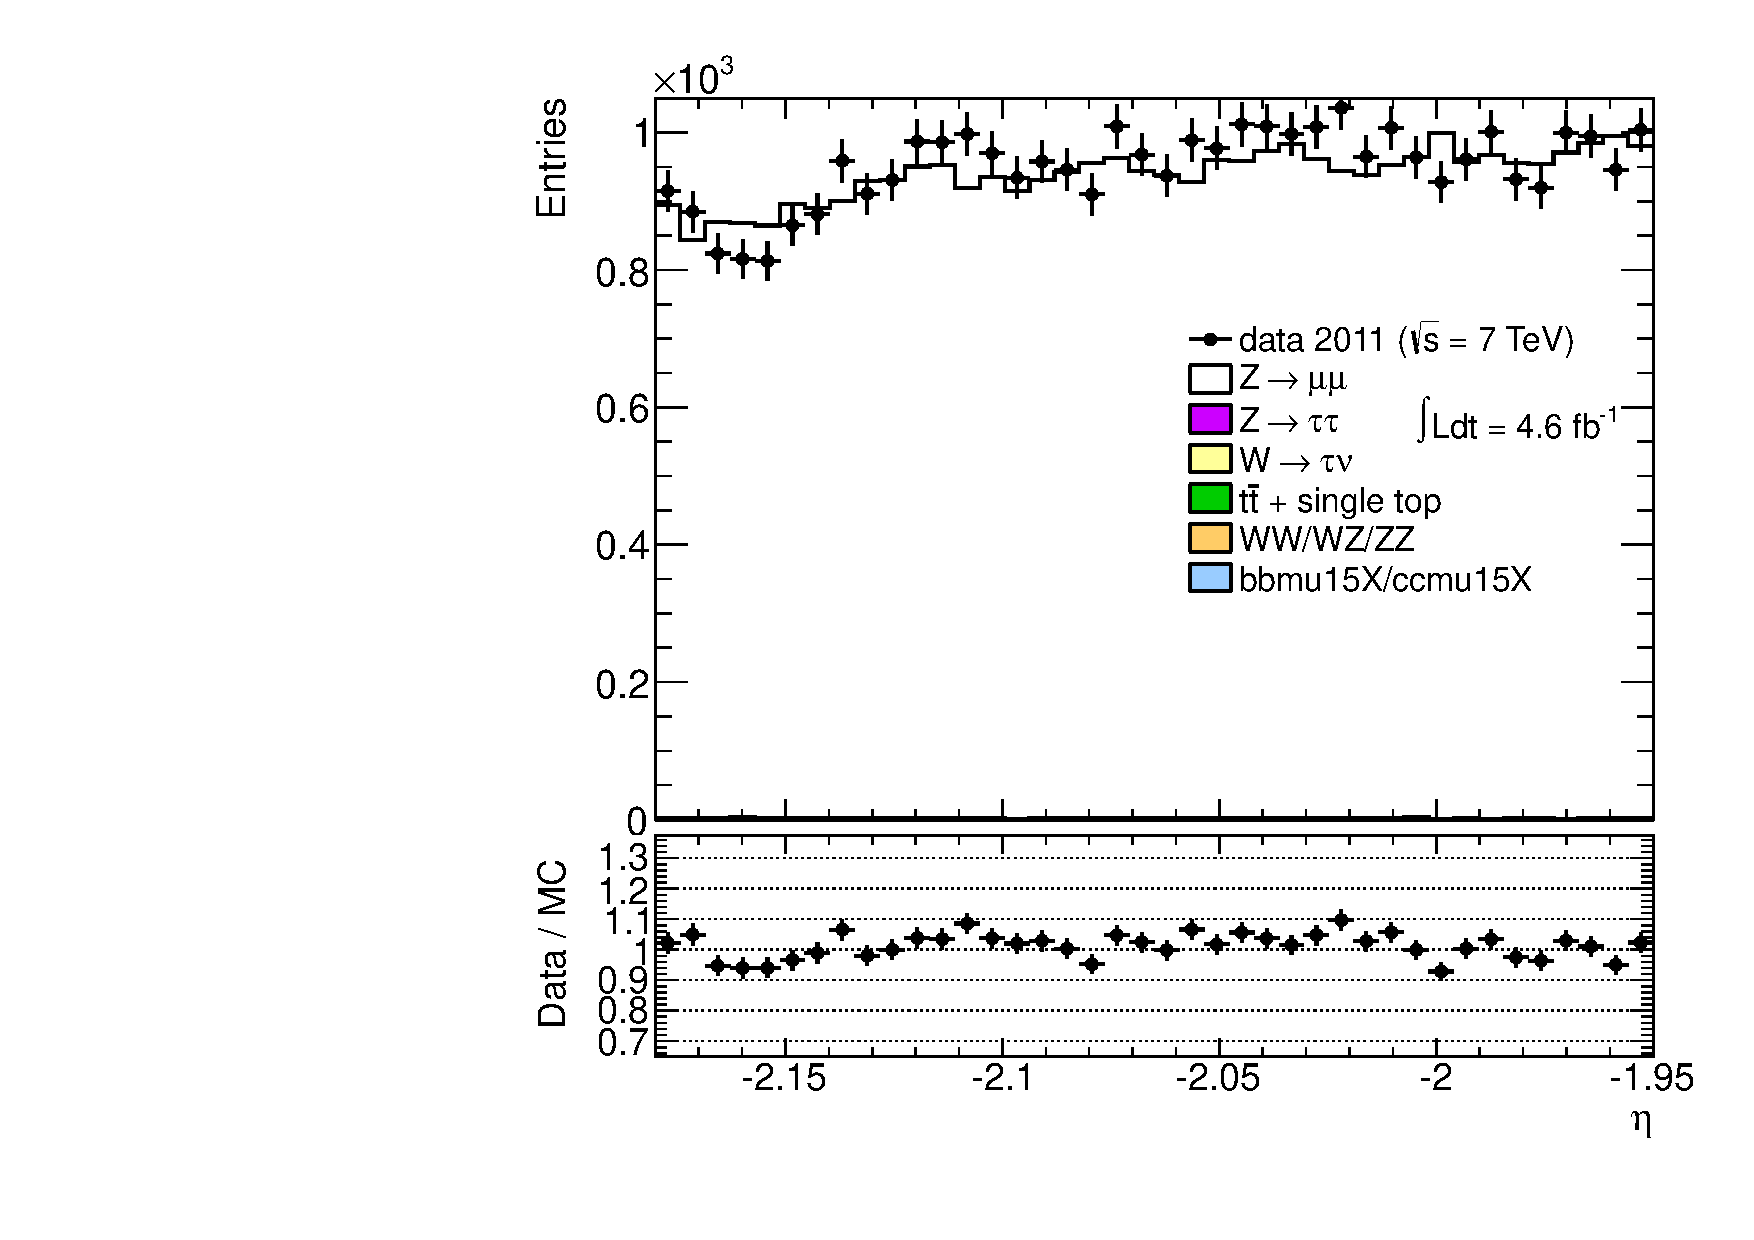
\includegraphics[width=0.66\textwidth]{dates/20130306/figures/both/Z_10_C_stack_lN_eta_ALL.pdf}
\column{.5\textwidth}
A-side (top: W; bottom: Z)
\centering
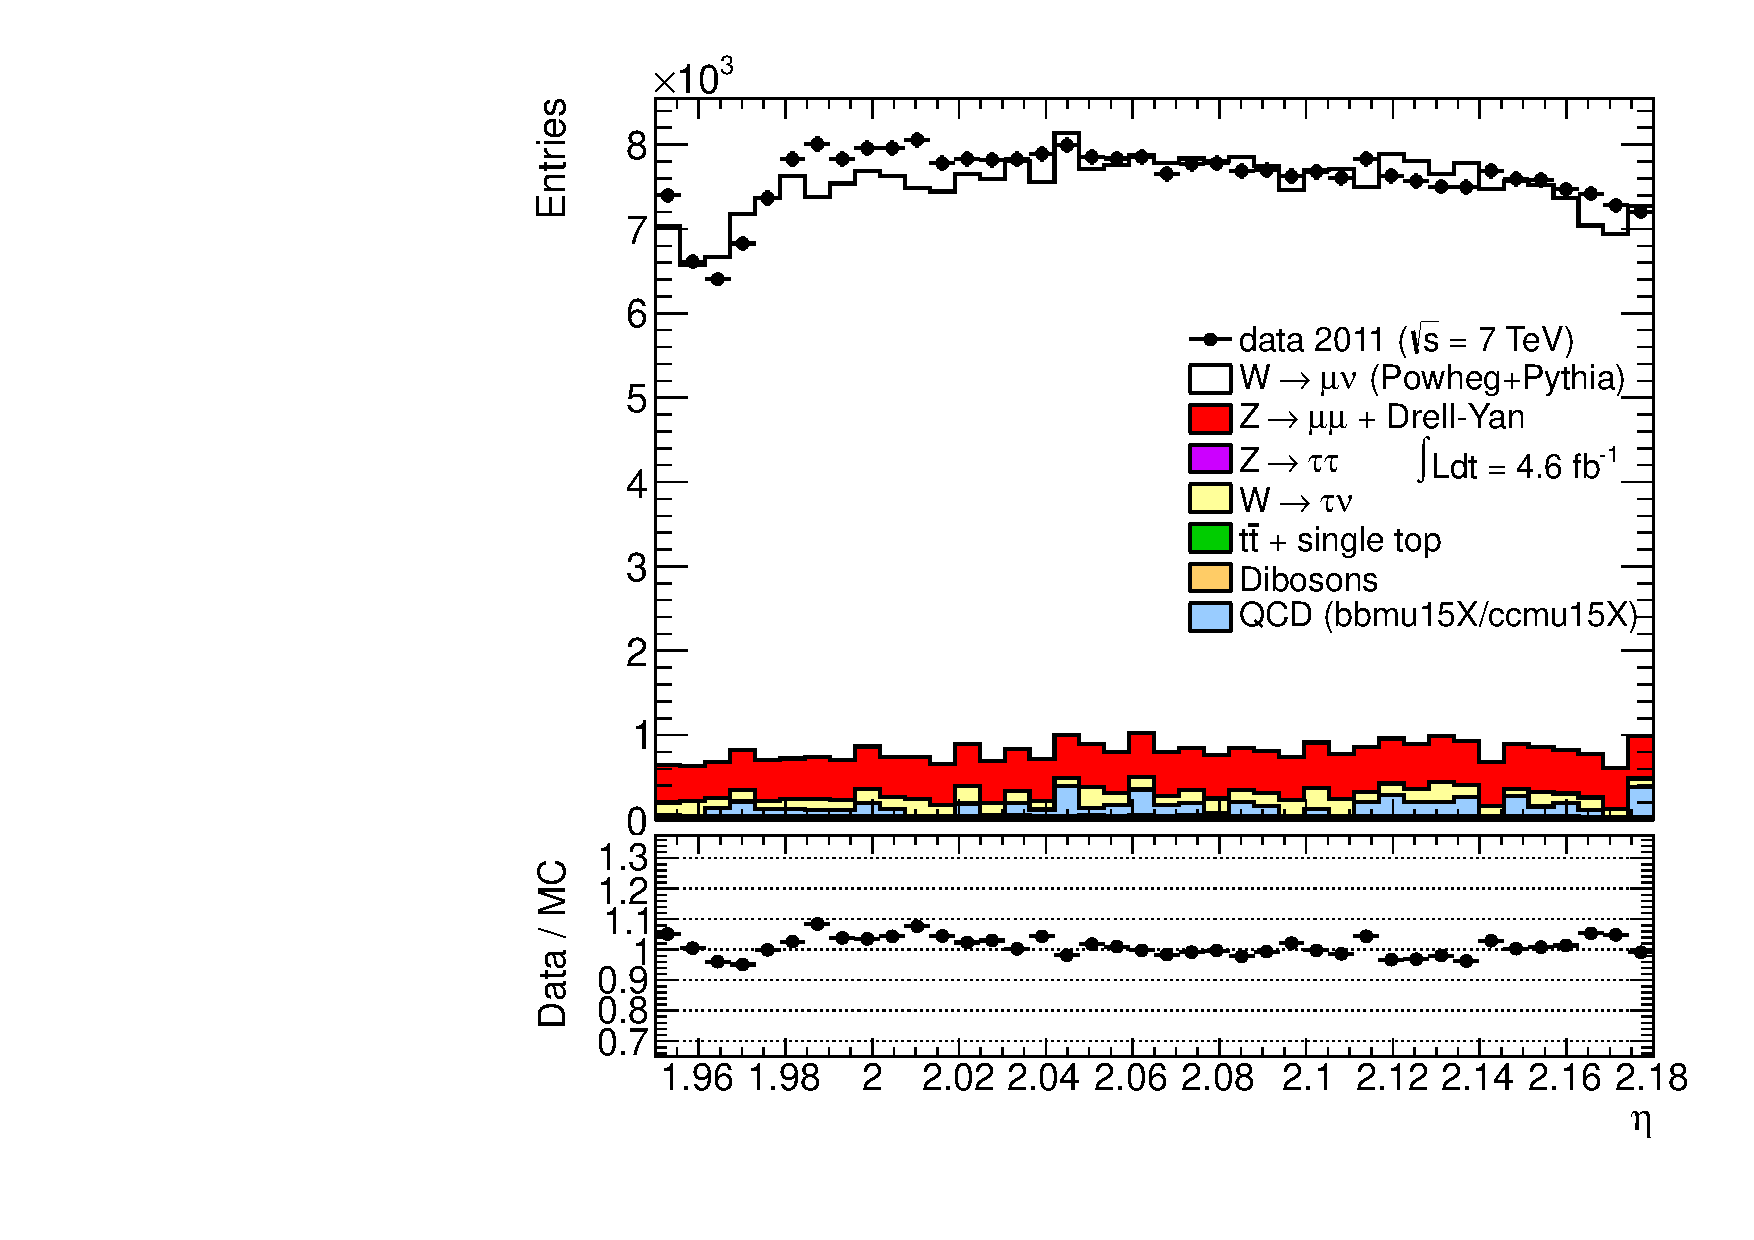
\includegraphics[width=0.66\textwidth]{dates/20130306/figures/both/W_10_A_stack_l_eta_NEG} \\
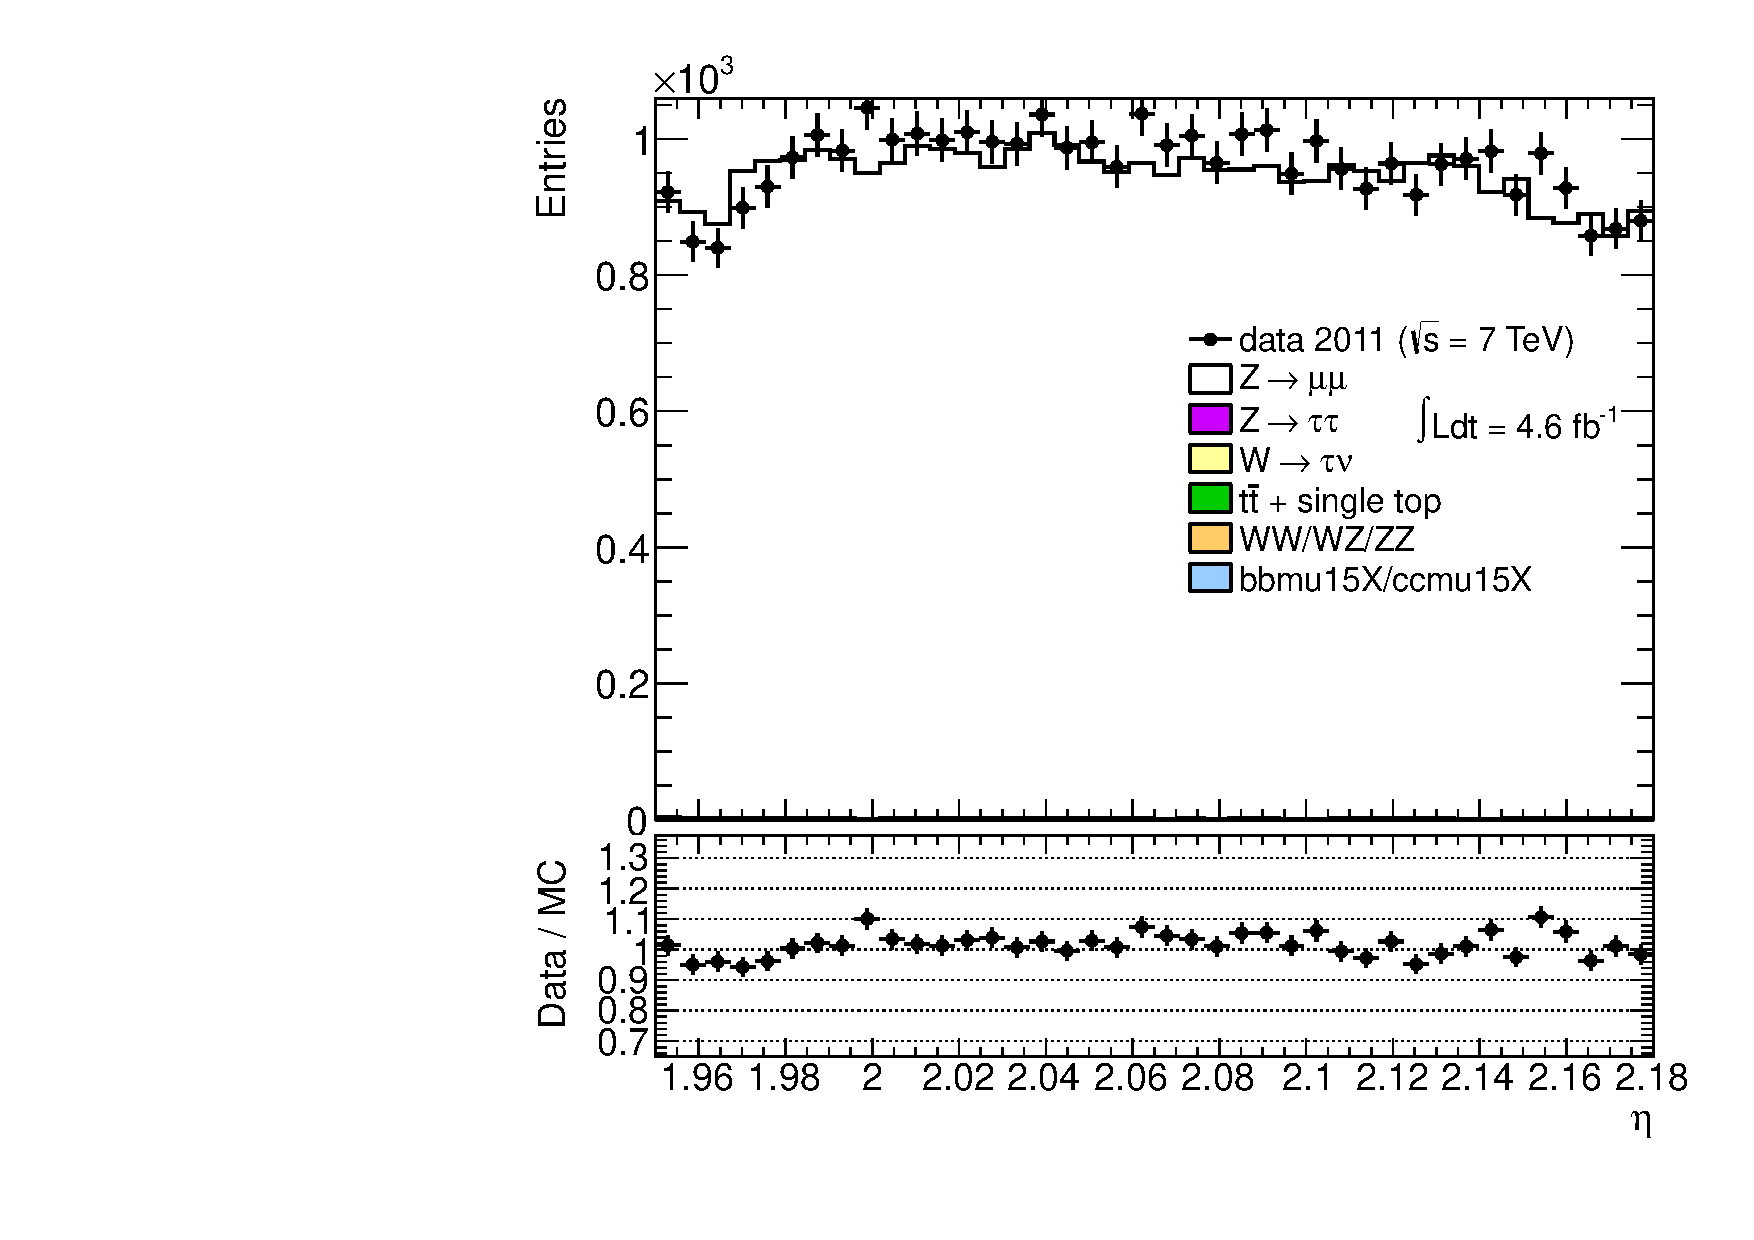
\includegraphics[width=0.66\textwidth]{dates/20130306/figures/both/Z_10_A_stack_lN_eta_ALL.pdf} 
\cole
}
\slide{ $\mu^{-}$: bin 10 ($1.95<\eta<2.18$), periods D-H } {
\colb[T]
\column{.5\textwidth}
C-side $\mu^{-}$ (top: W; bottom: Z)
\centering
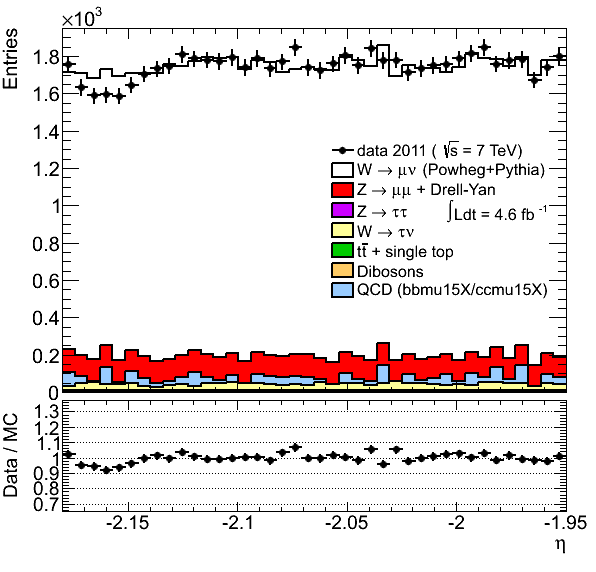
\includegraphics[width=0.66\textwidth]{dates/20130306/figures/both/WpDtoH_10_C_stack_l_eta_NEG} \\
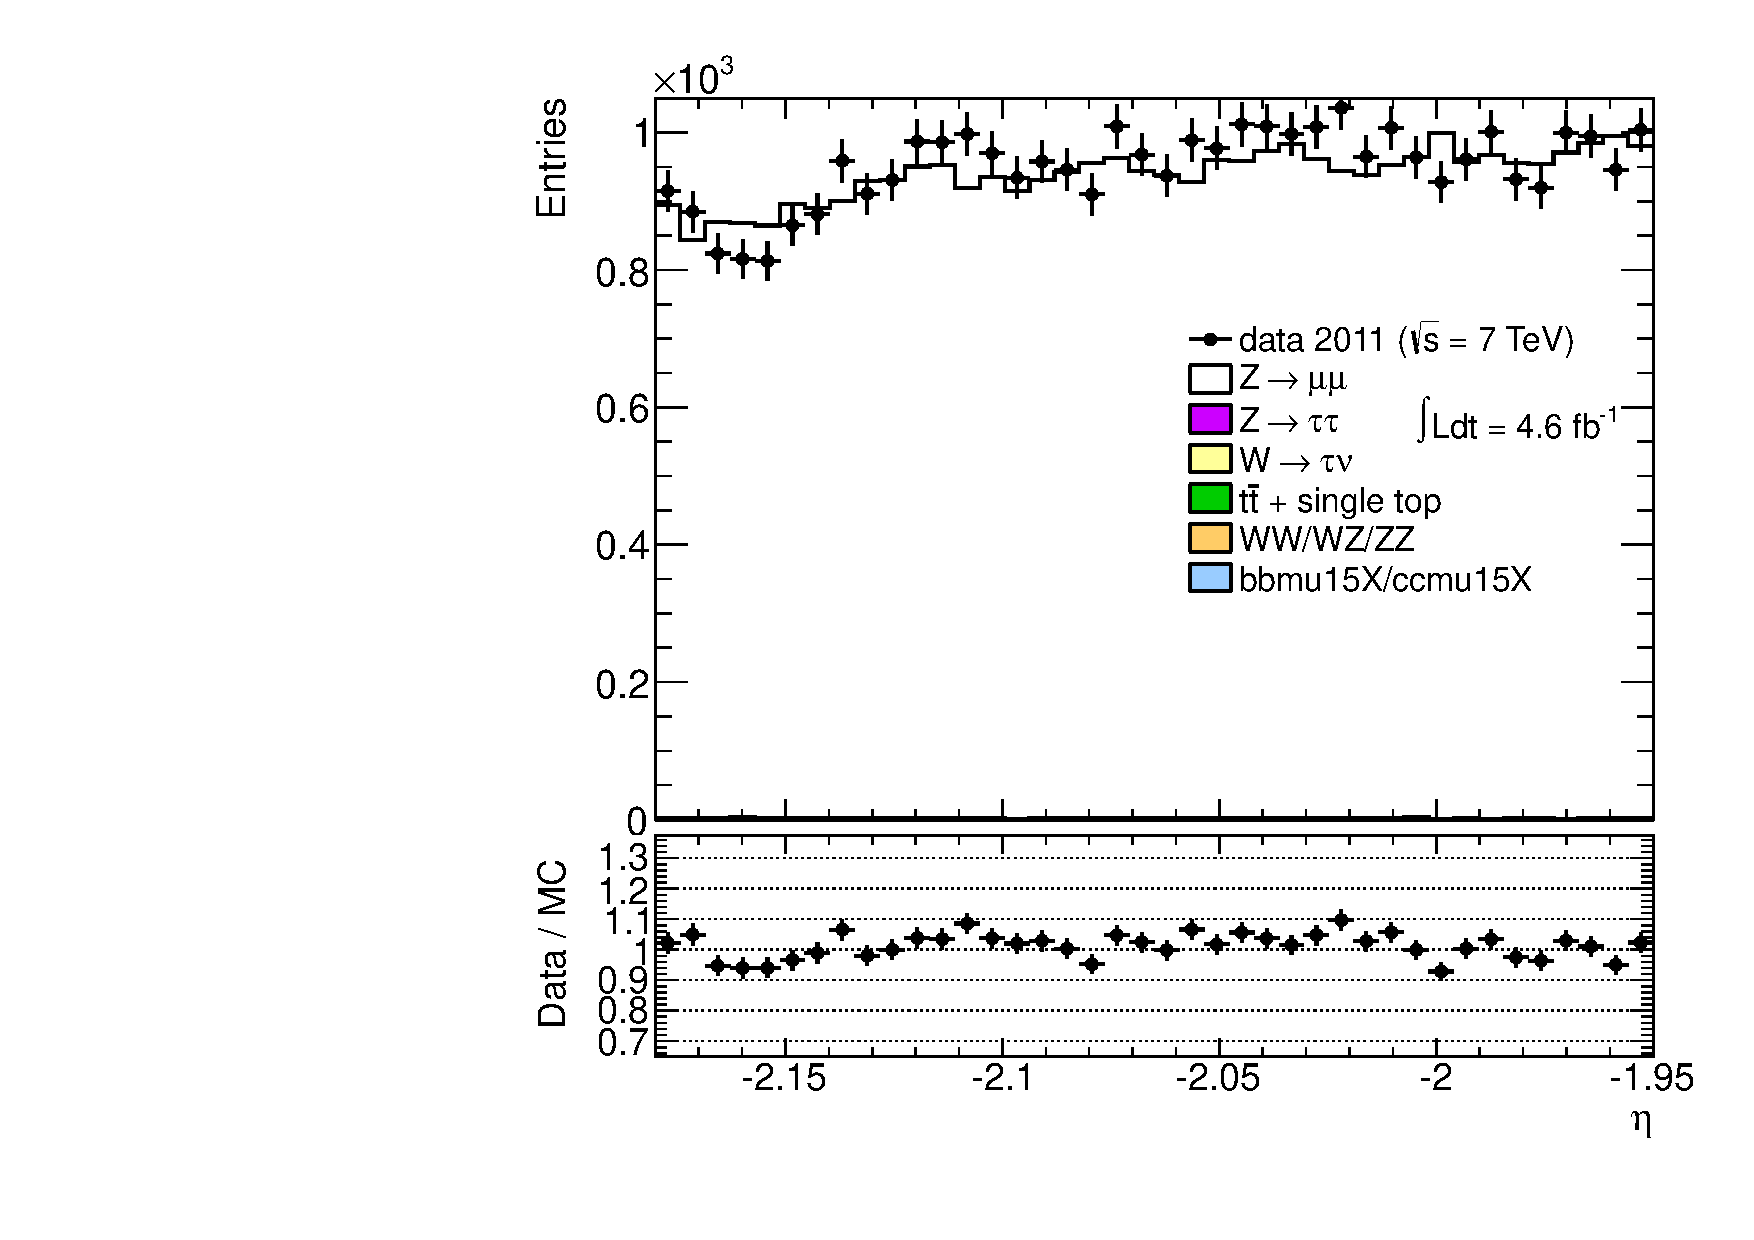
\includegraphics[width=0.66\textwidth]{dates/20130306/figures/both/Z_10_C_stack_lN_eta_ALL.pdf}
\column{.5\textwidth}
A-side $\mu^{-}$ (top: W; bottom: Z)
\centering
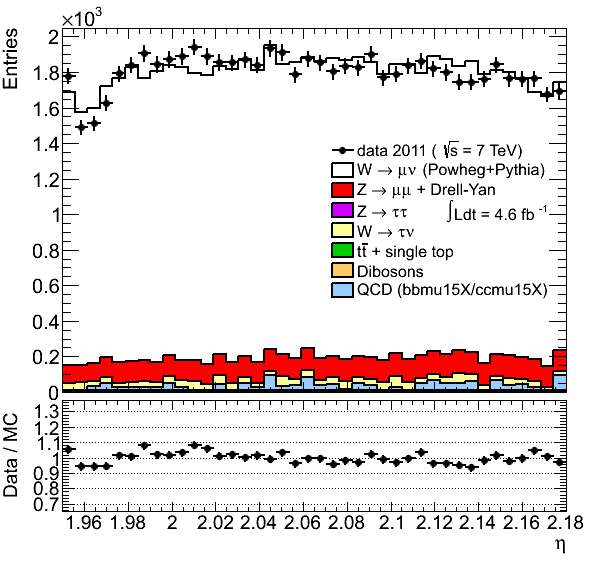
\includegraphics[width=0.66\textwidth]{dates/20130306/figures/both/WpDtoH_10_A_stack_l_eta_NEG} \\
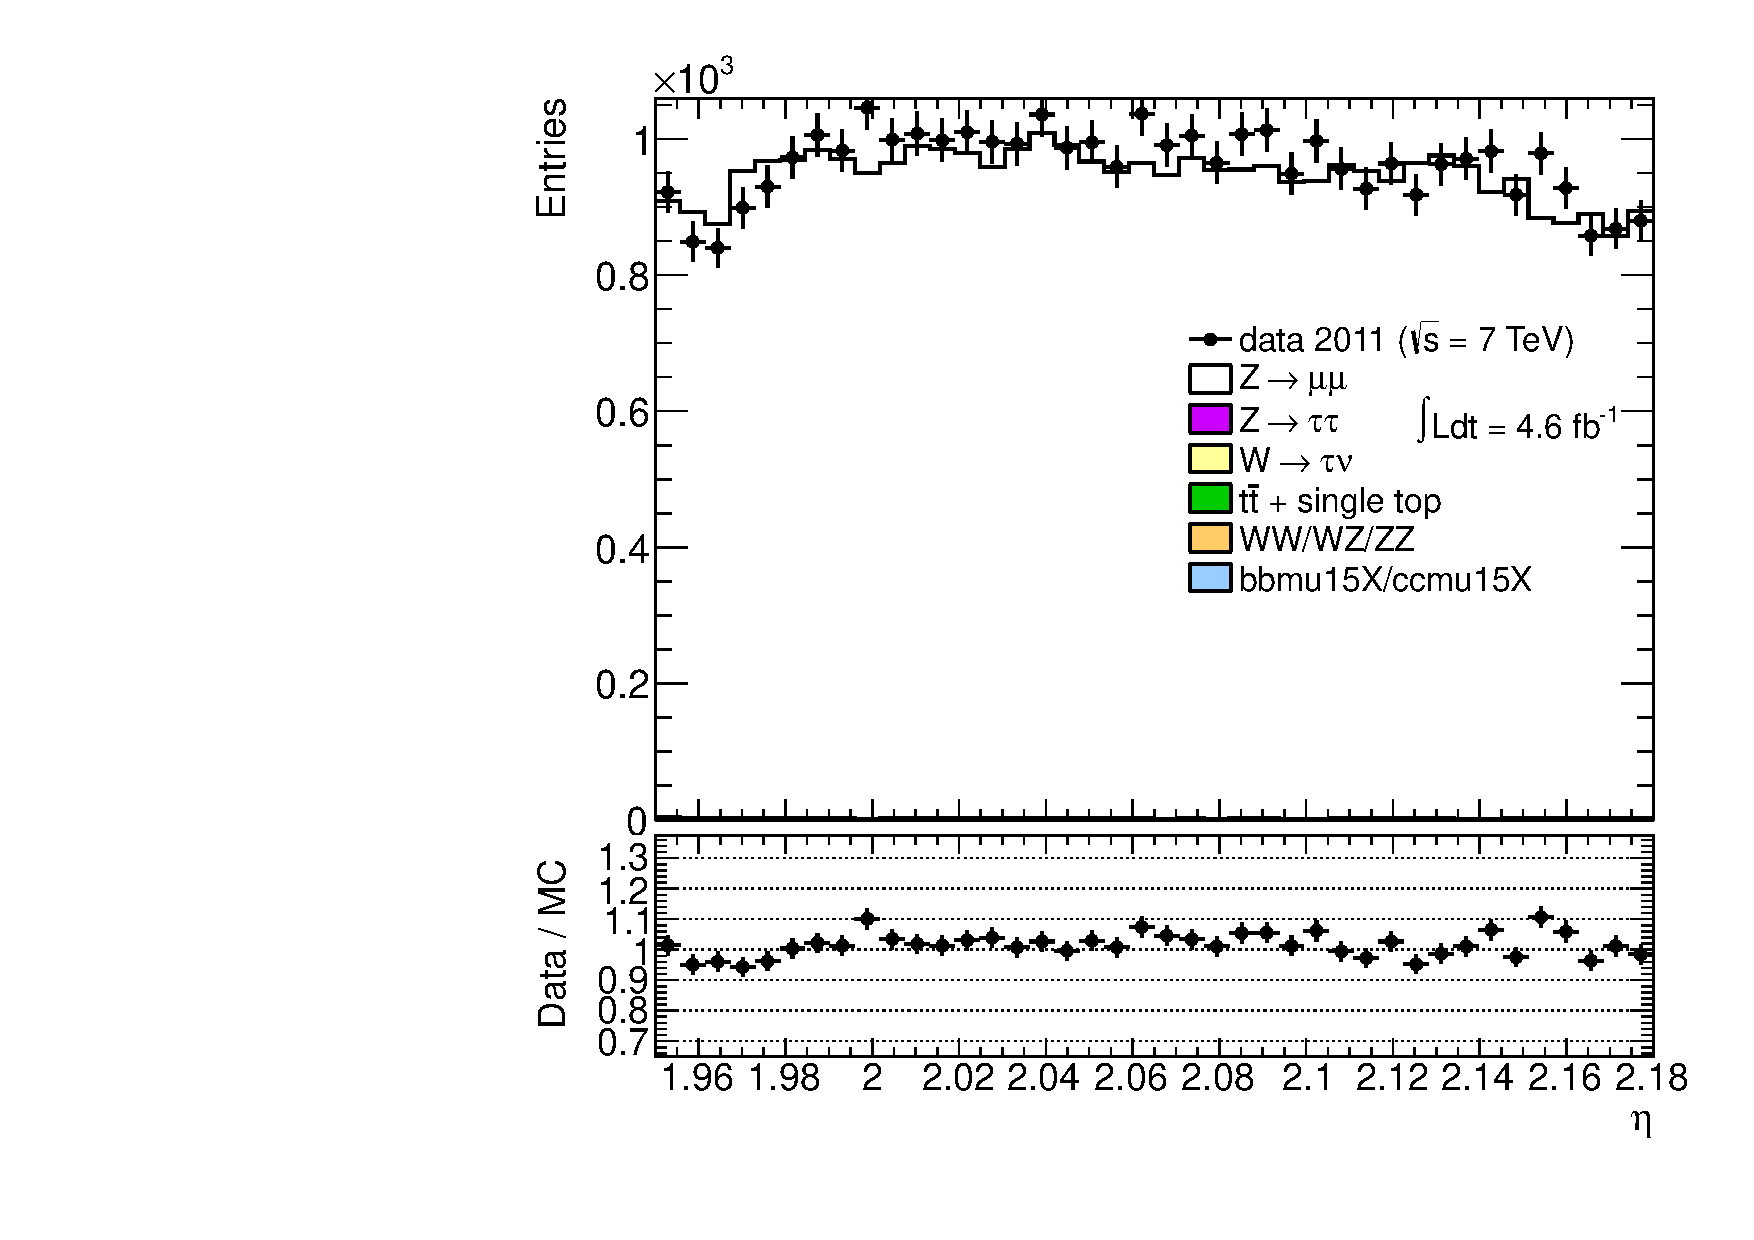
\includegraphics[width=0.66\textwidth]{dates/20130306/figures/both/Z_10_A_stack_lN_eta_ALL.pdf} 
\cole
}
\slide{ $\mu^{-}$: bin 10 ($1.95<\eta<2.18$), period I } {
\colb[T]
\column{.5\textwidth}
C-side $\mu^{-}$ (top: W; bottom: Z)
\centering
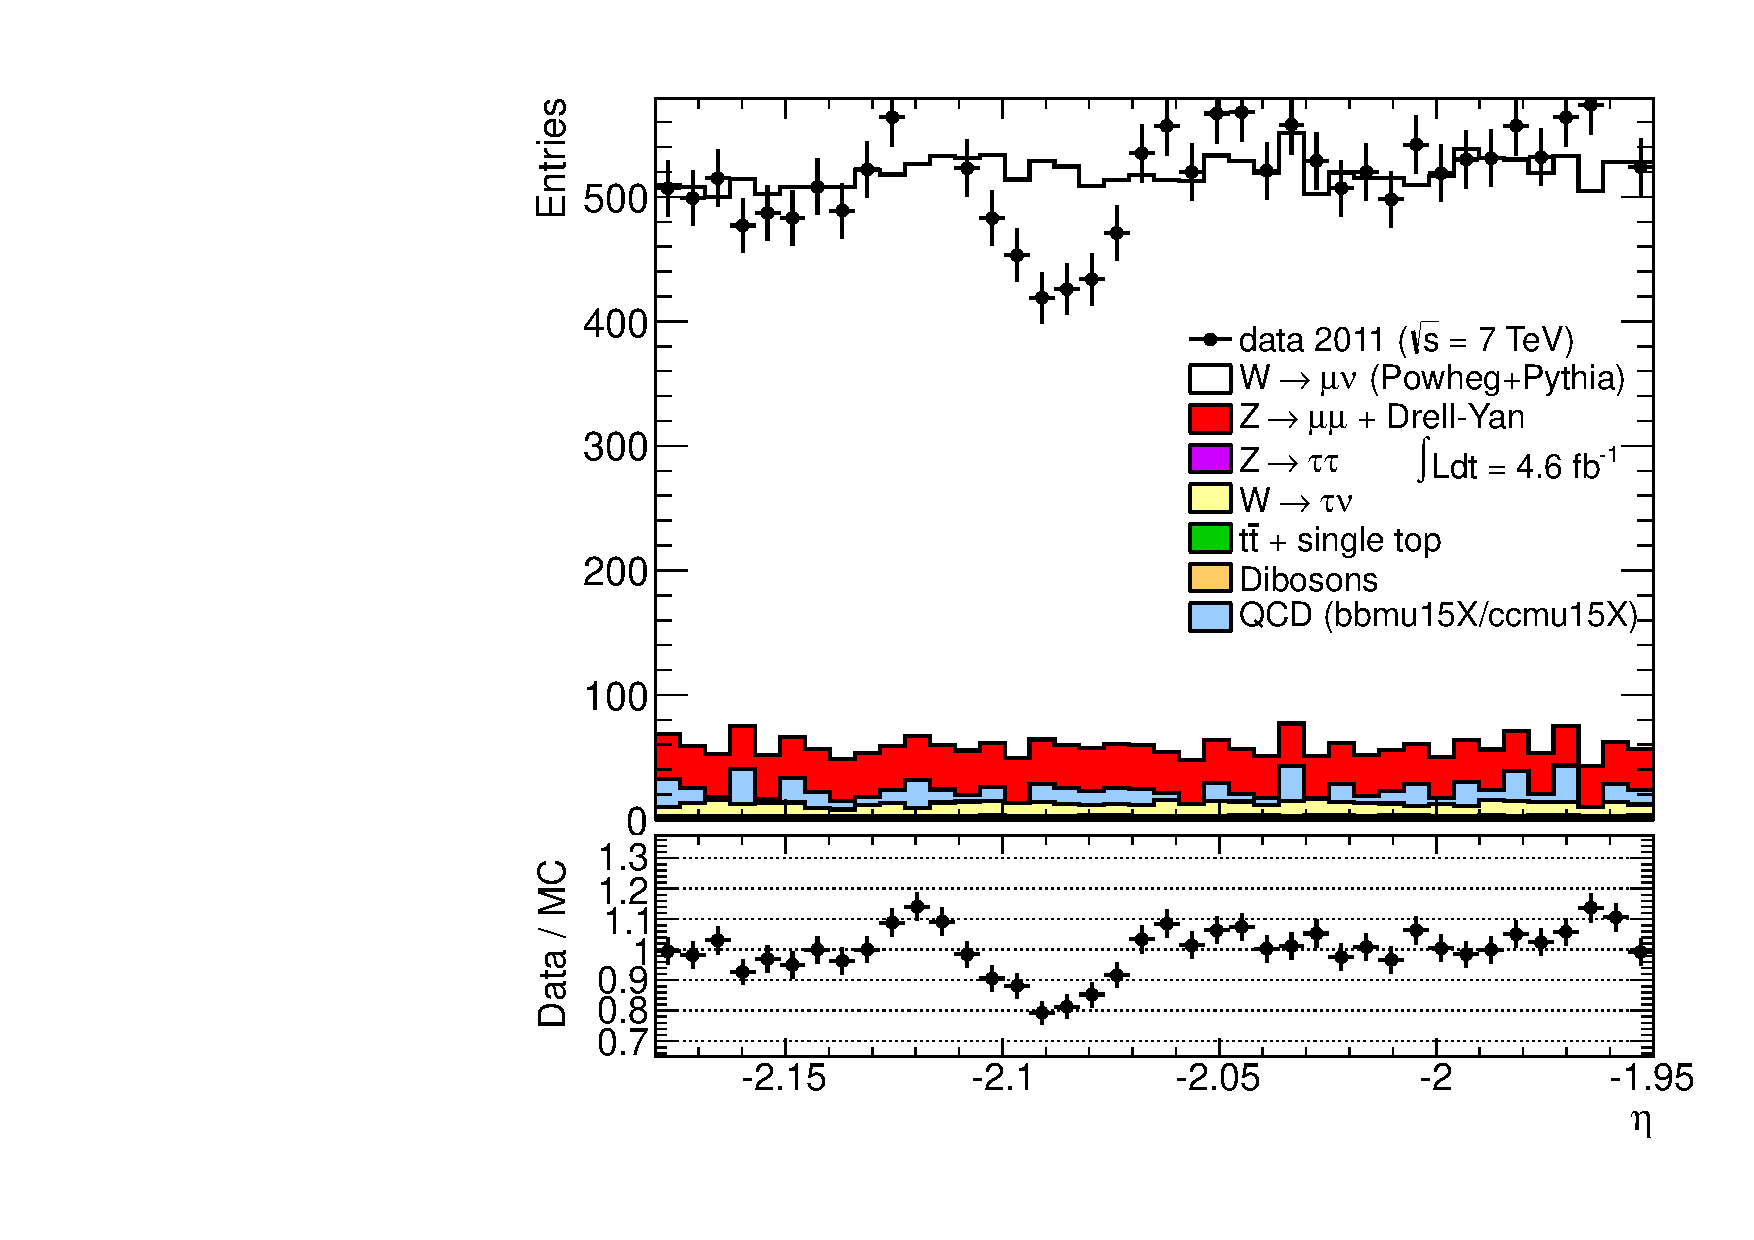
\includegraphics[width=0.66\textwidth]{dates/20130306/figures/both/WpItoI_10_C_stack_l_eta_NEG} \\
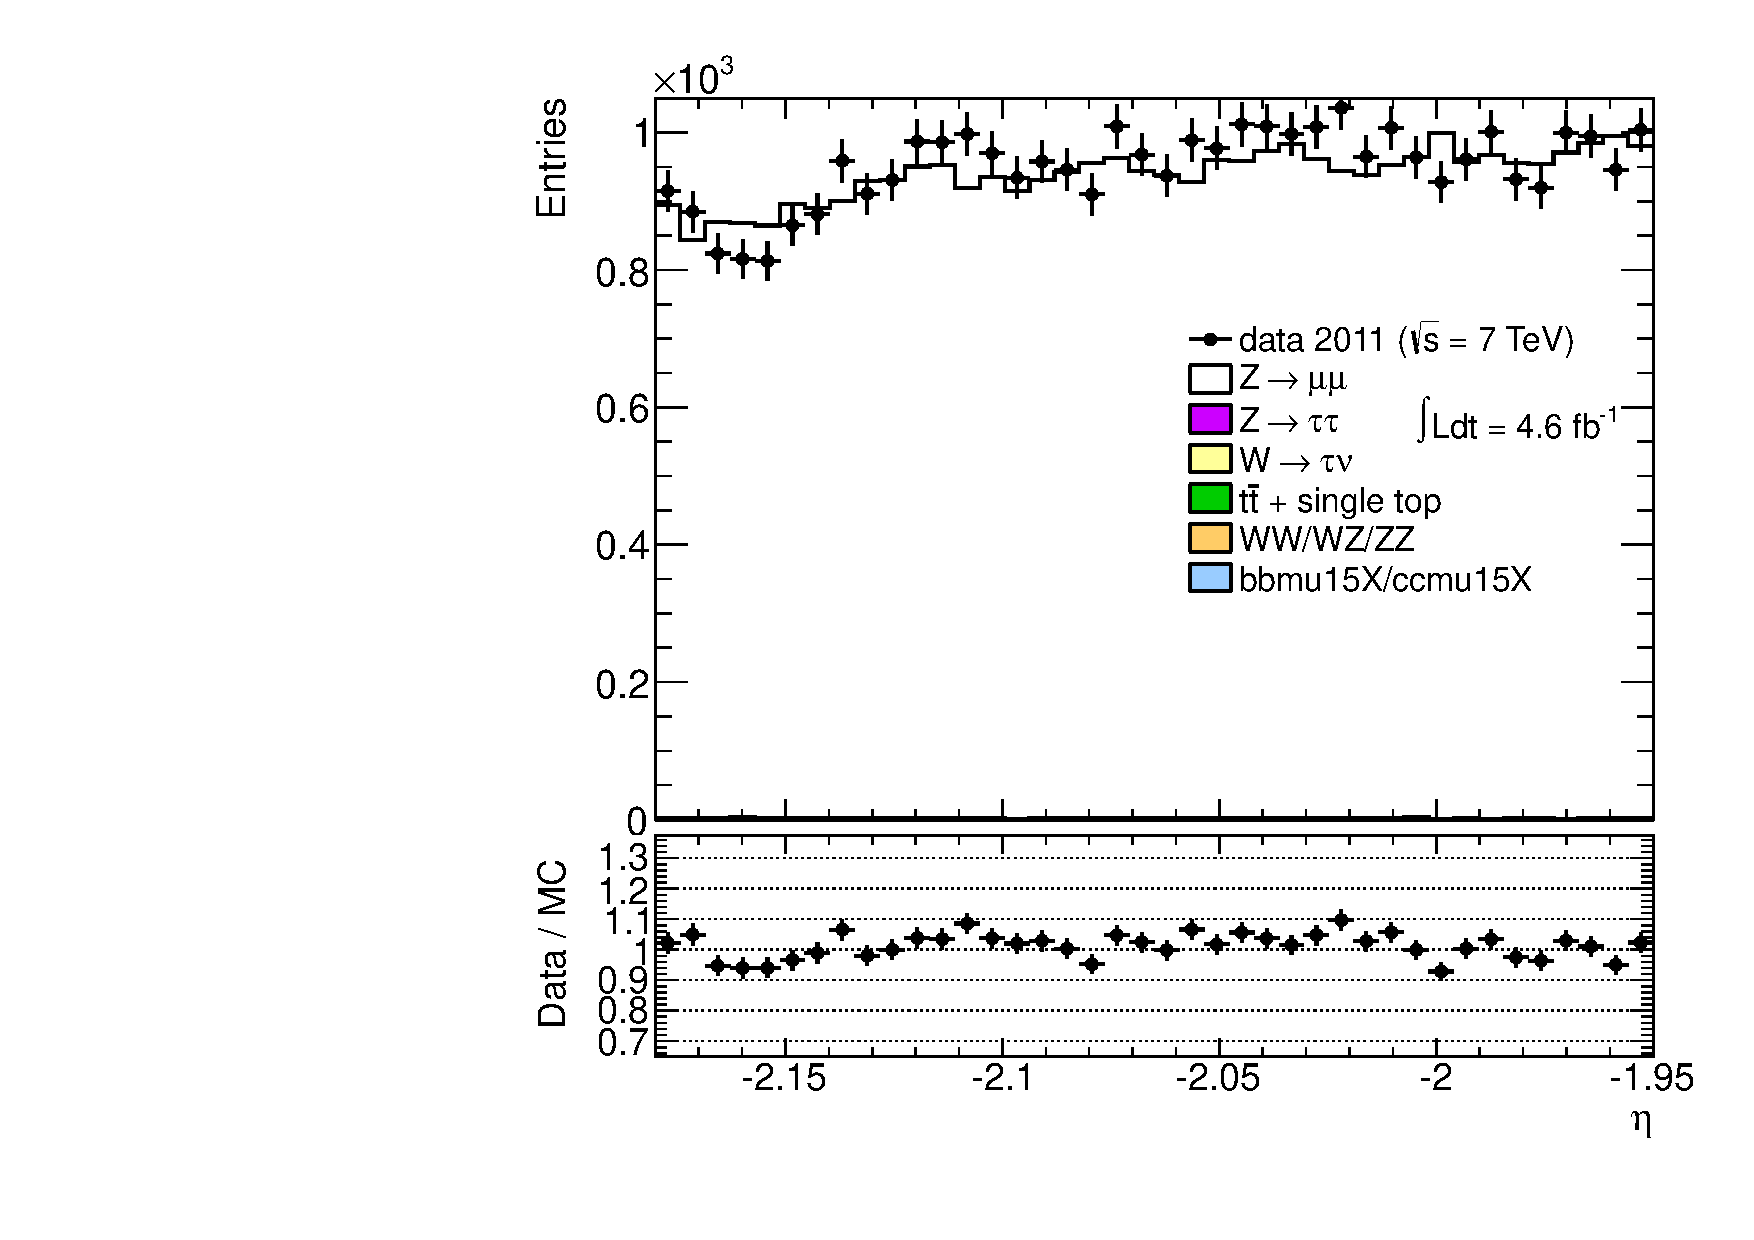
\includegraphics[width=0.66\textwidth]{dates/20130306/figures/both/Z_10_C_stack_lN_eta_ALL.pdf}
\column{.5\textwidth}
A-side $\mu^{-}$ (top: W; bottom: Z)
\centering
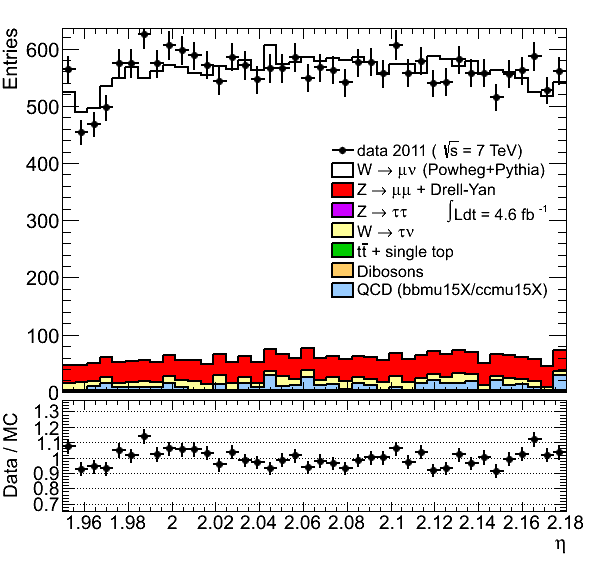
\includegraphics[width=0.66\textwidth]{dates/20130306/figures/both/WpItoI_10_A_stack_l_eta_NEG} \\
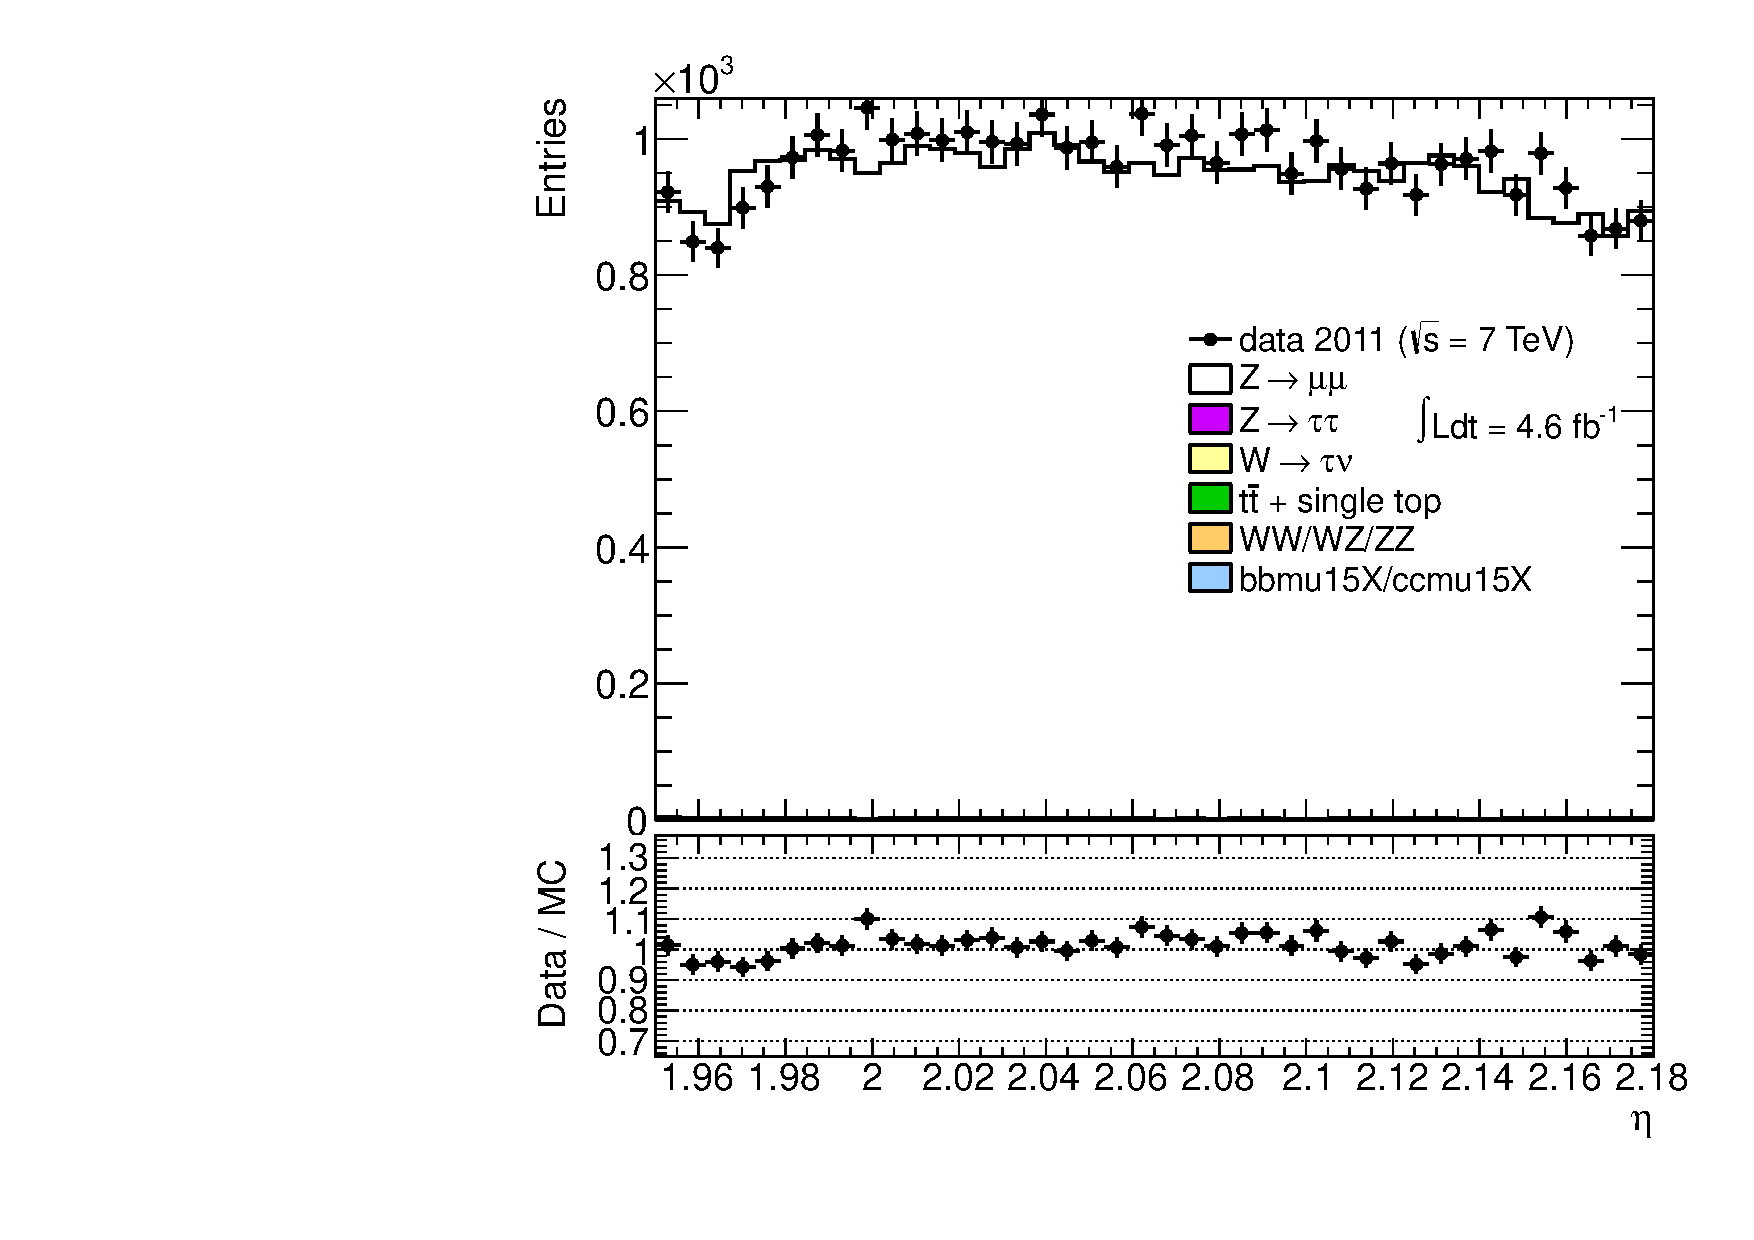
\includegraphics[width=0.66\textwidth]{dates/20130306/figures/both/Z_10_A_stack_lN_eta_ALL.pdf} 
\cole
}
\slide{ $\mu^{-}$: bin 10 ($1.95<\eta<2.18$), periods I-K } {
\colb[T]
\column{.5\textwidth}
C-side $\mu^{-}$ (top: W; bottom: Z)
\centering
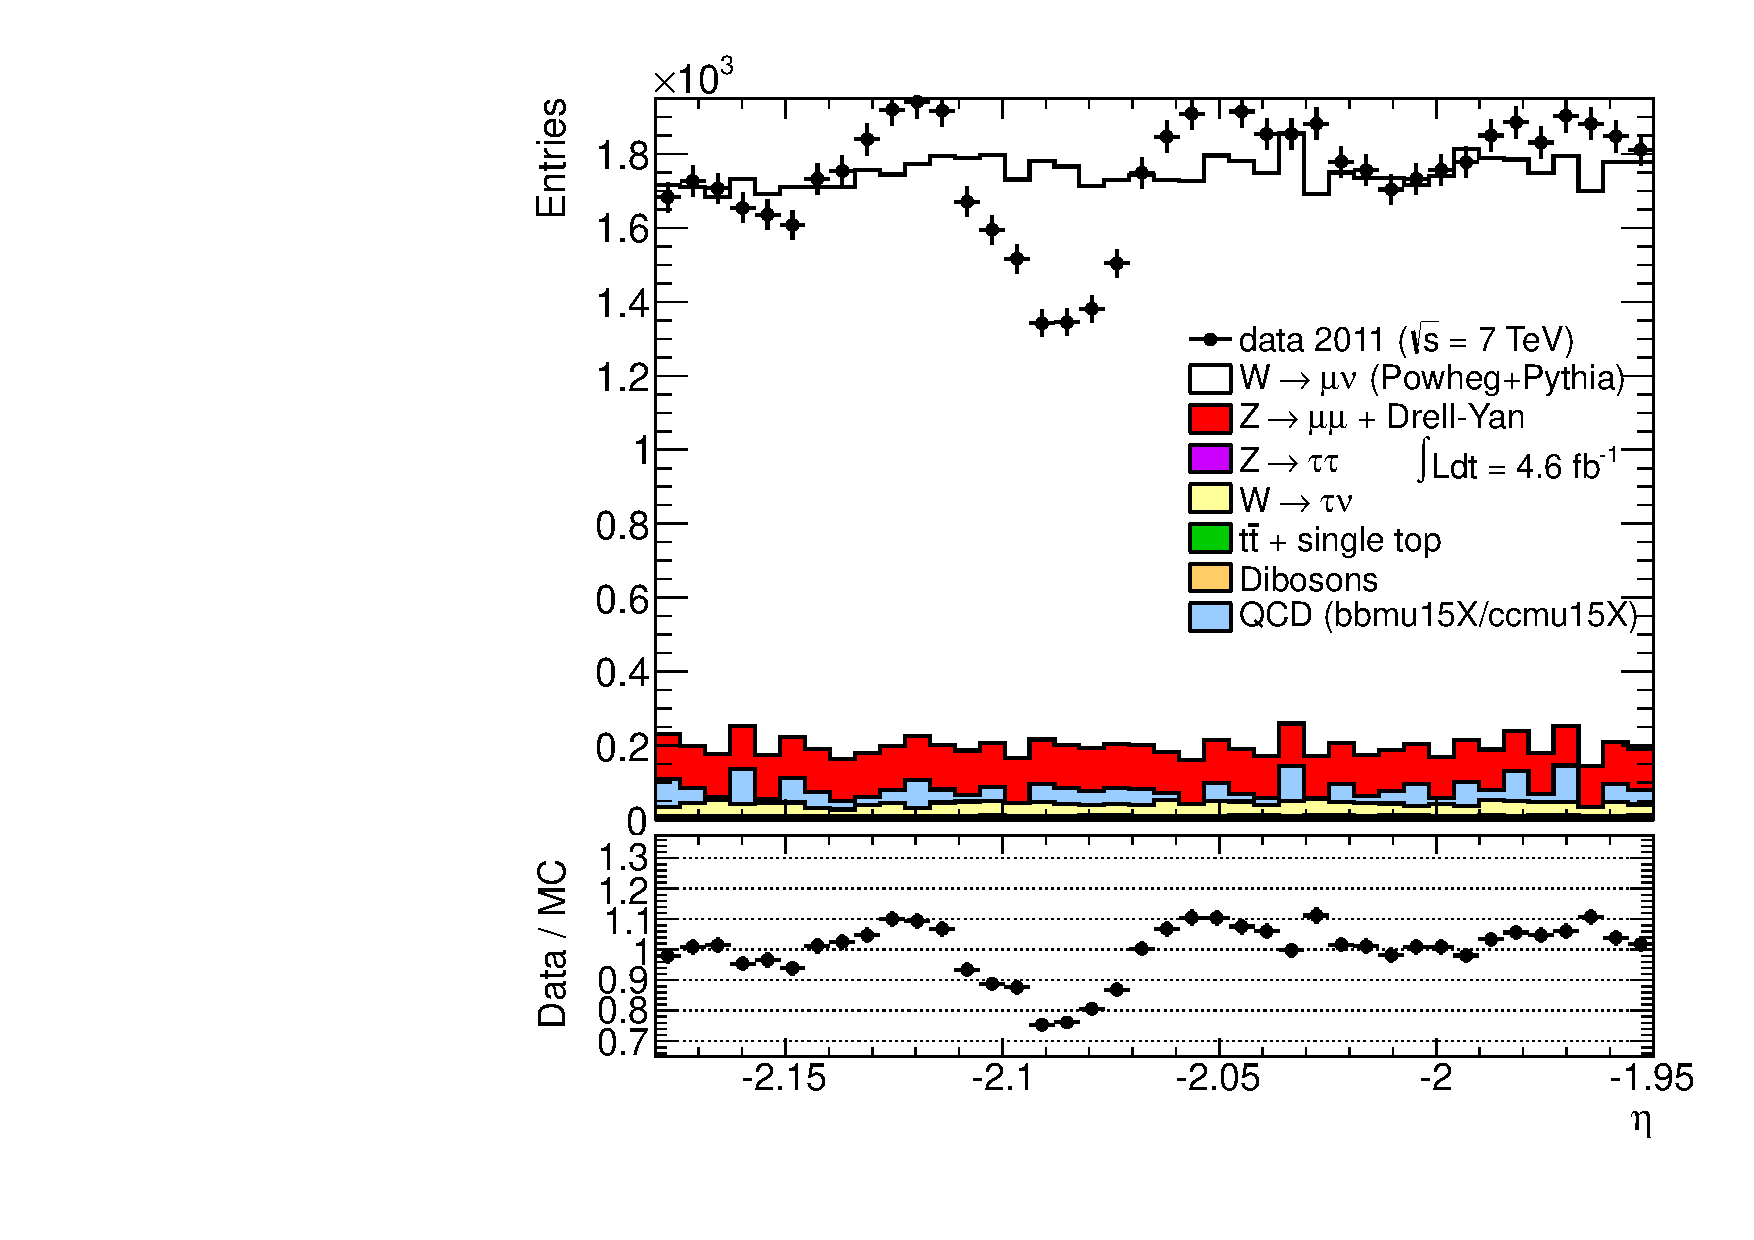
\includegraphics[width=0.66\textwidth]{dates/20130306/figures/both/WpItoK_10_C_stack_l_eta_NEG} \\
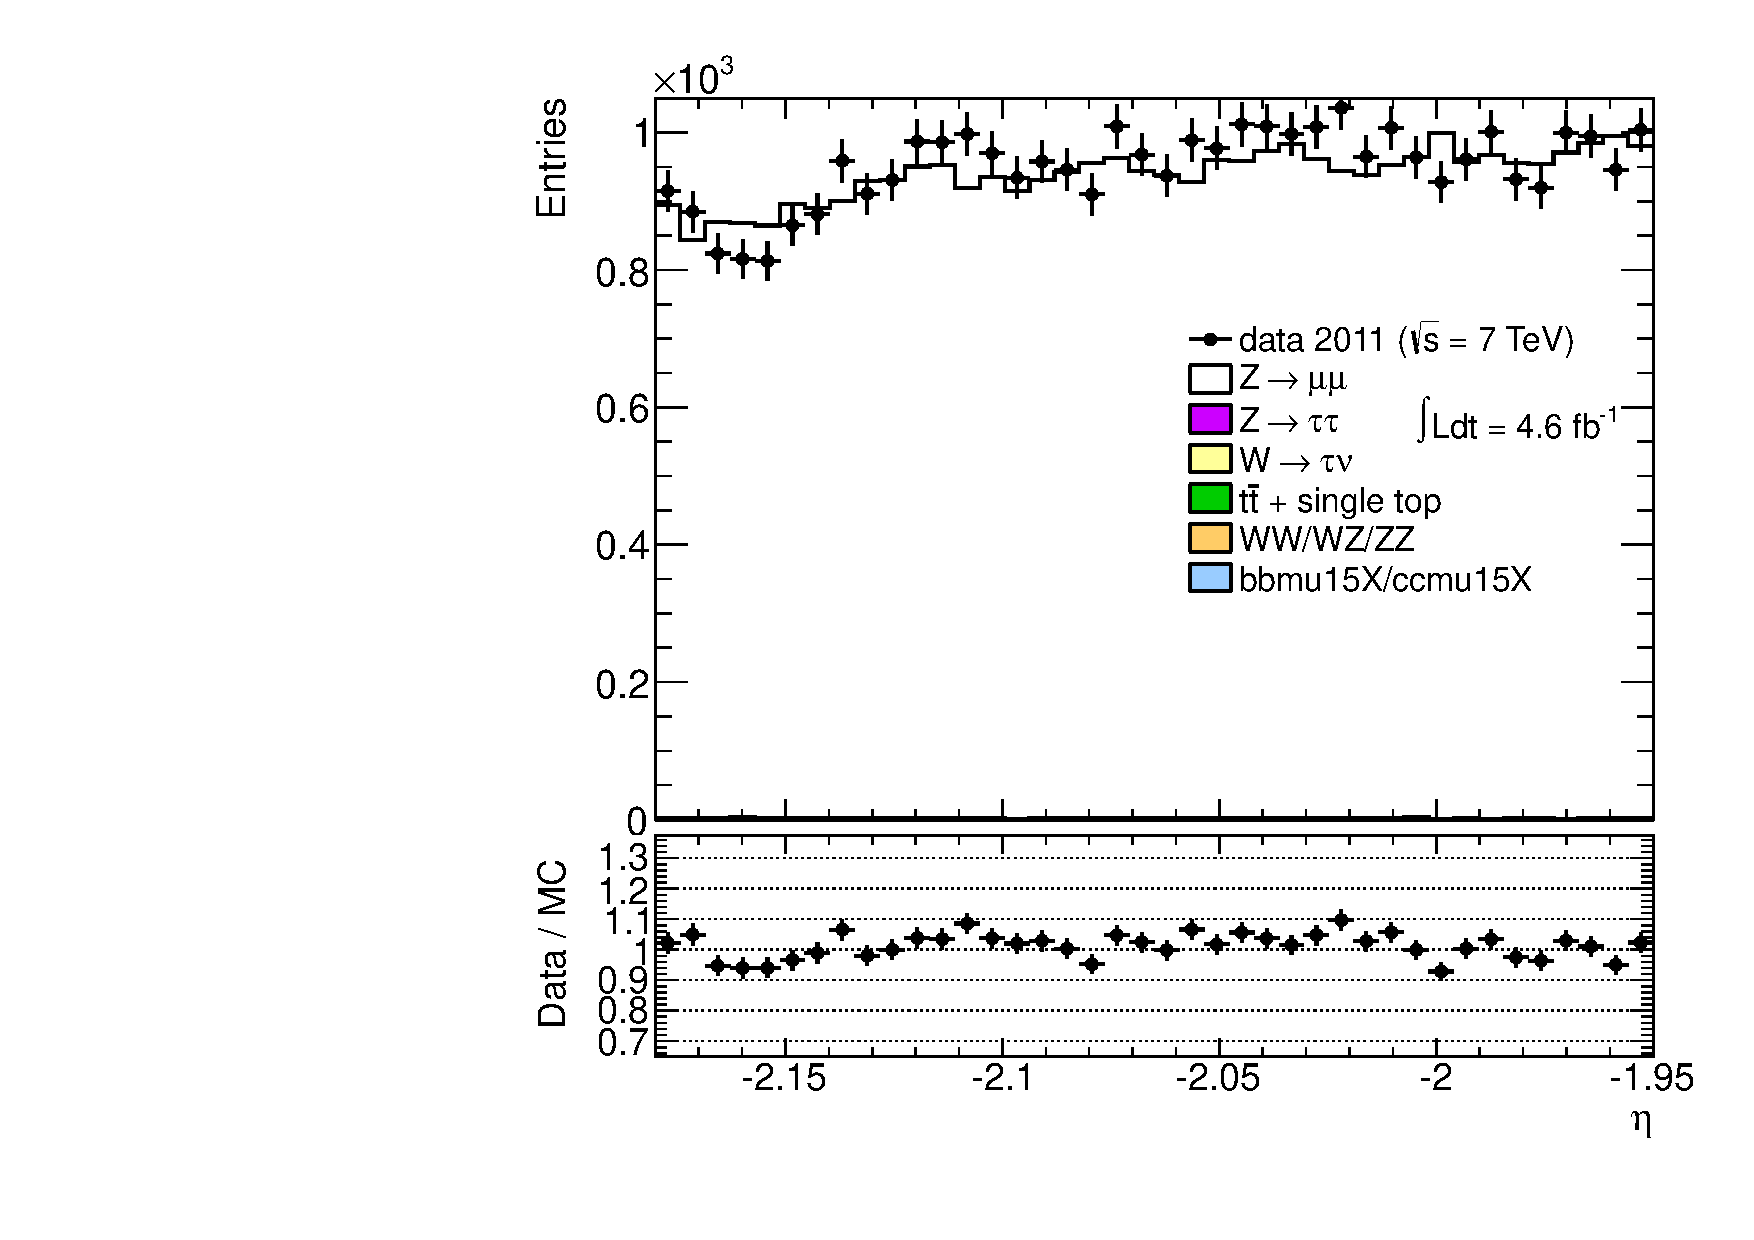
\includegraphics[width=0.66\textwidth]{dates/20130306/figures/both/Z_10_C_stack_lN_eta_ALL.pdf}
\column{.5\textwidth}
A-side $\mu^{-}$ (top: W; bottom: Z)
\centering
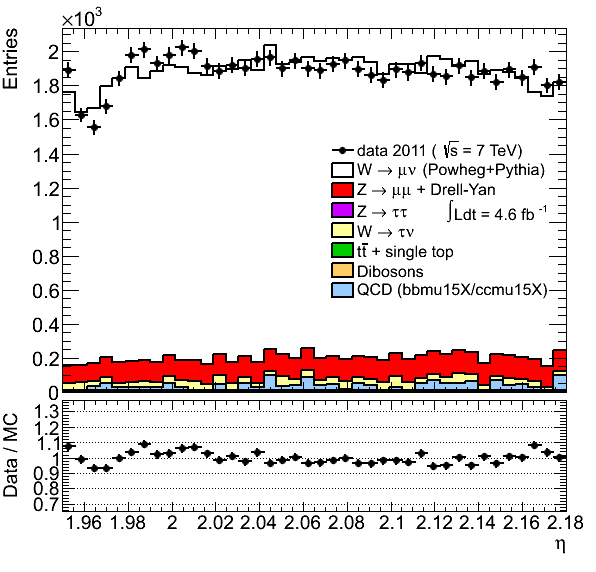
\includegraphics[width=0.66\textwidth]{dates/20130306/figures/both/WpItoK_10_A_stack_l_eta_NEG} \\
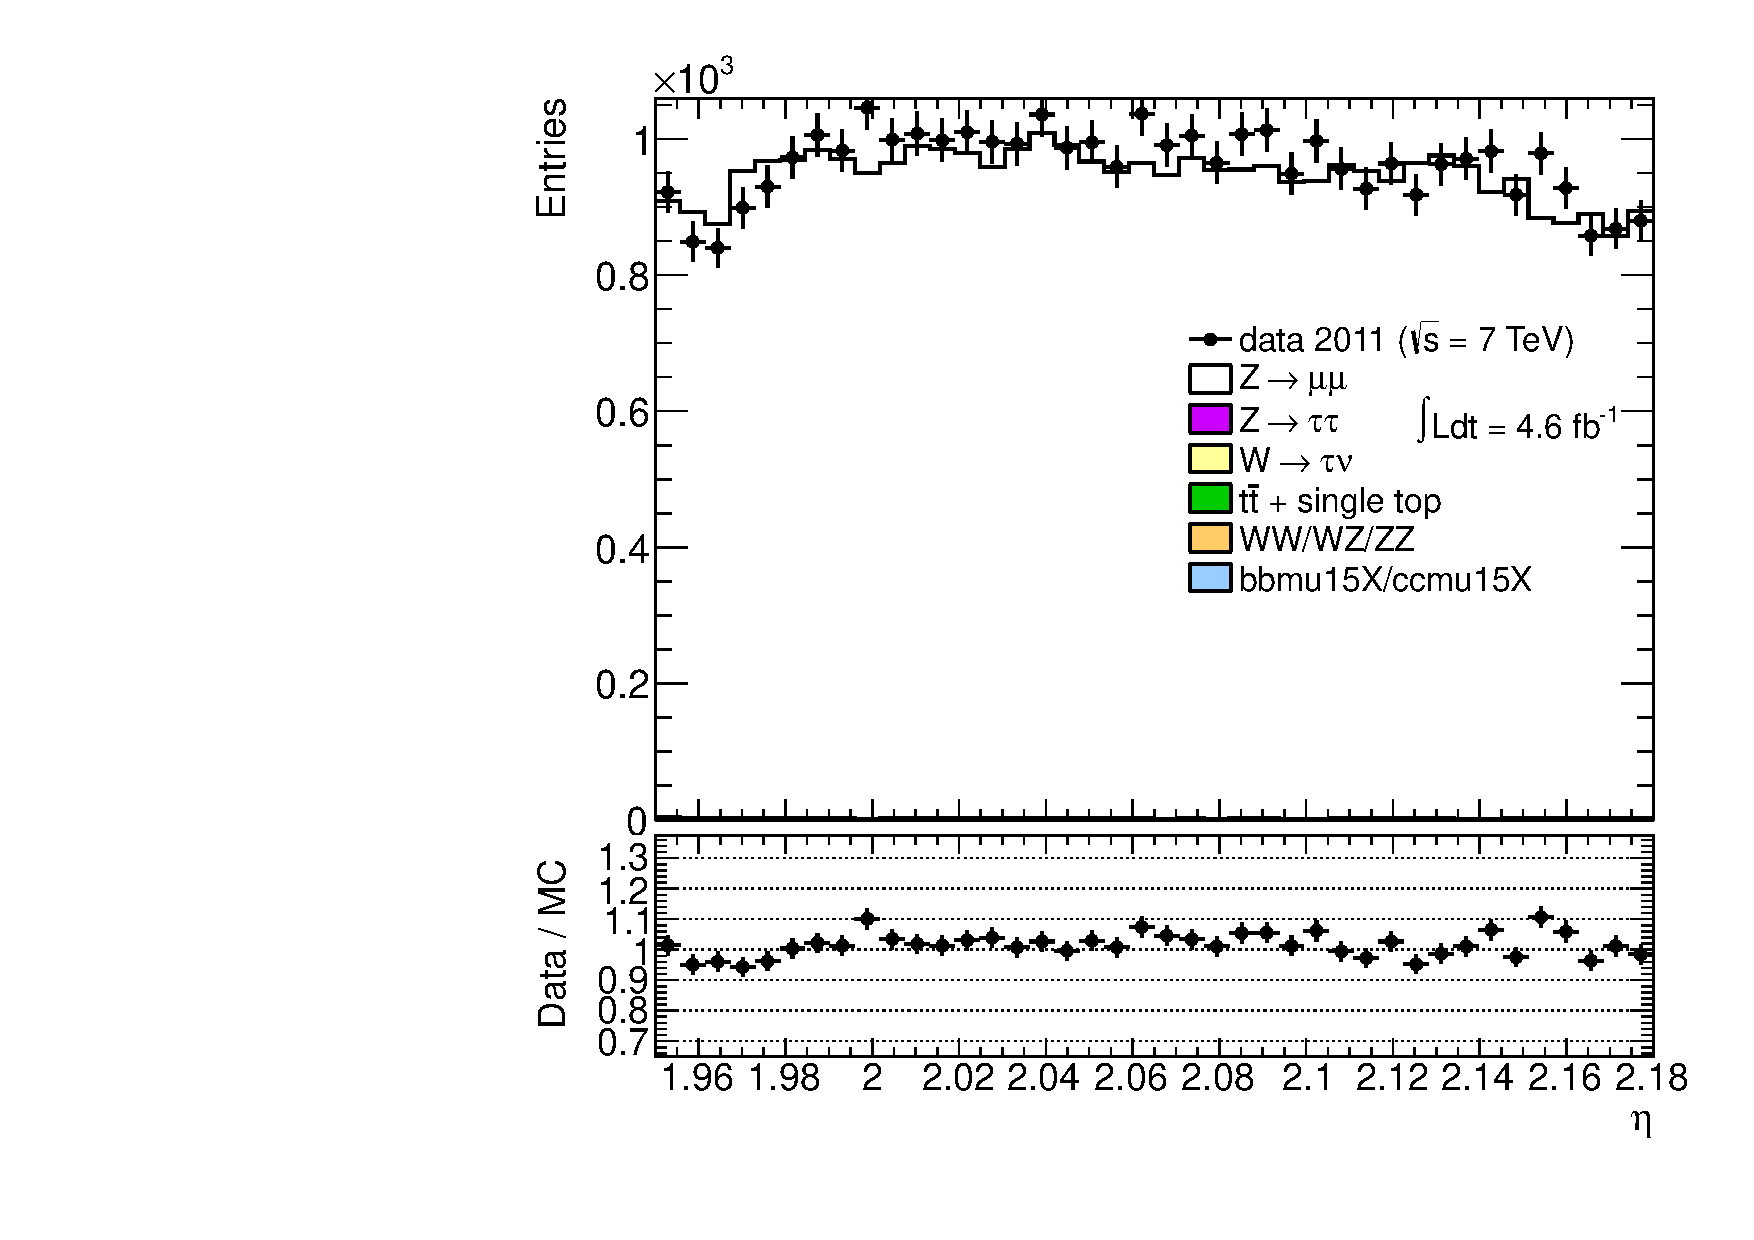
\includegraphics[width=0.66\textwidth]{dates/20130306/figures/both/Z_10_A_stack_lN_eta_ALL.pdf} 
\cole
}
\slide{ $\mu^{-}$: bin 10 ($1.95<\eta<2.18$), period L } {
\colb[T]
\column{.5\textwidth}
C-side $\mu^{-}$ (top: W; bottom: Z)
\centering
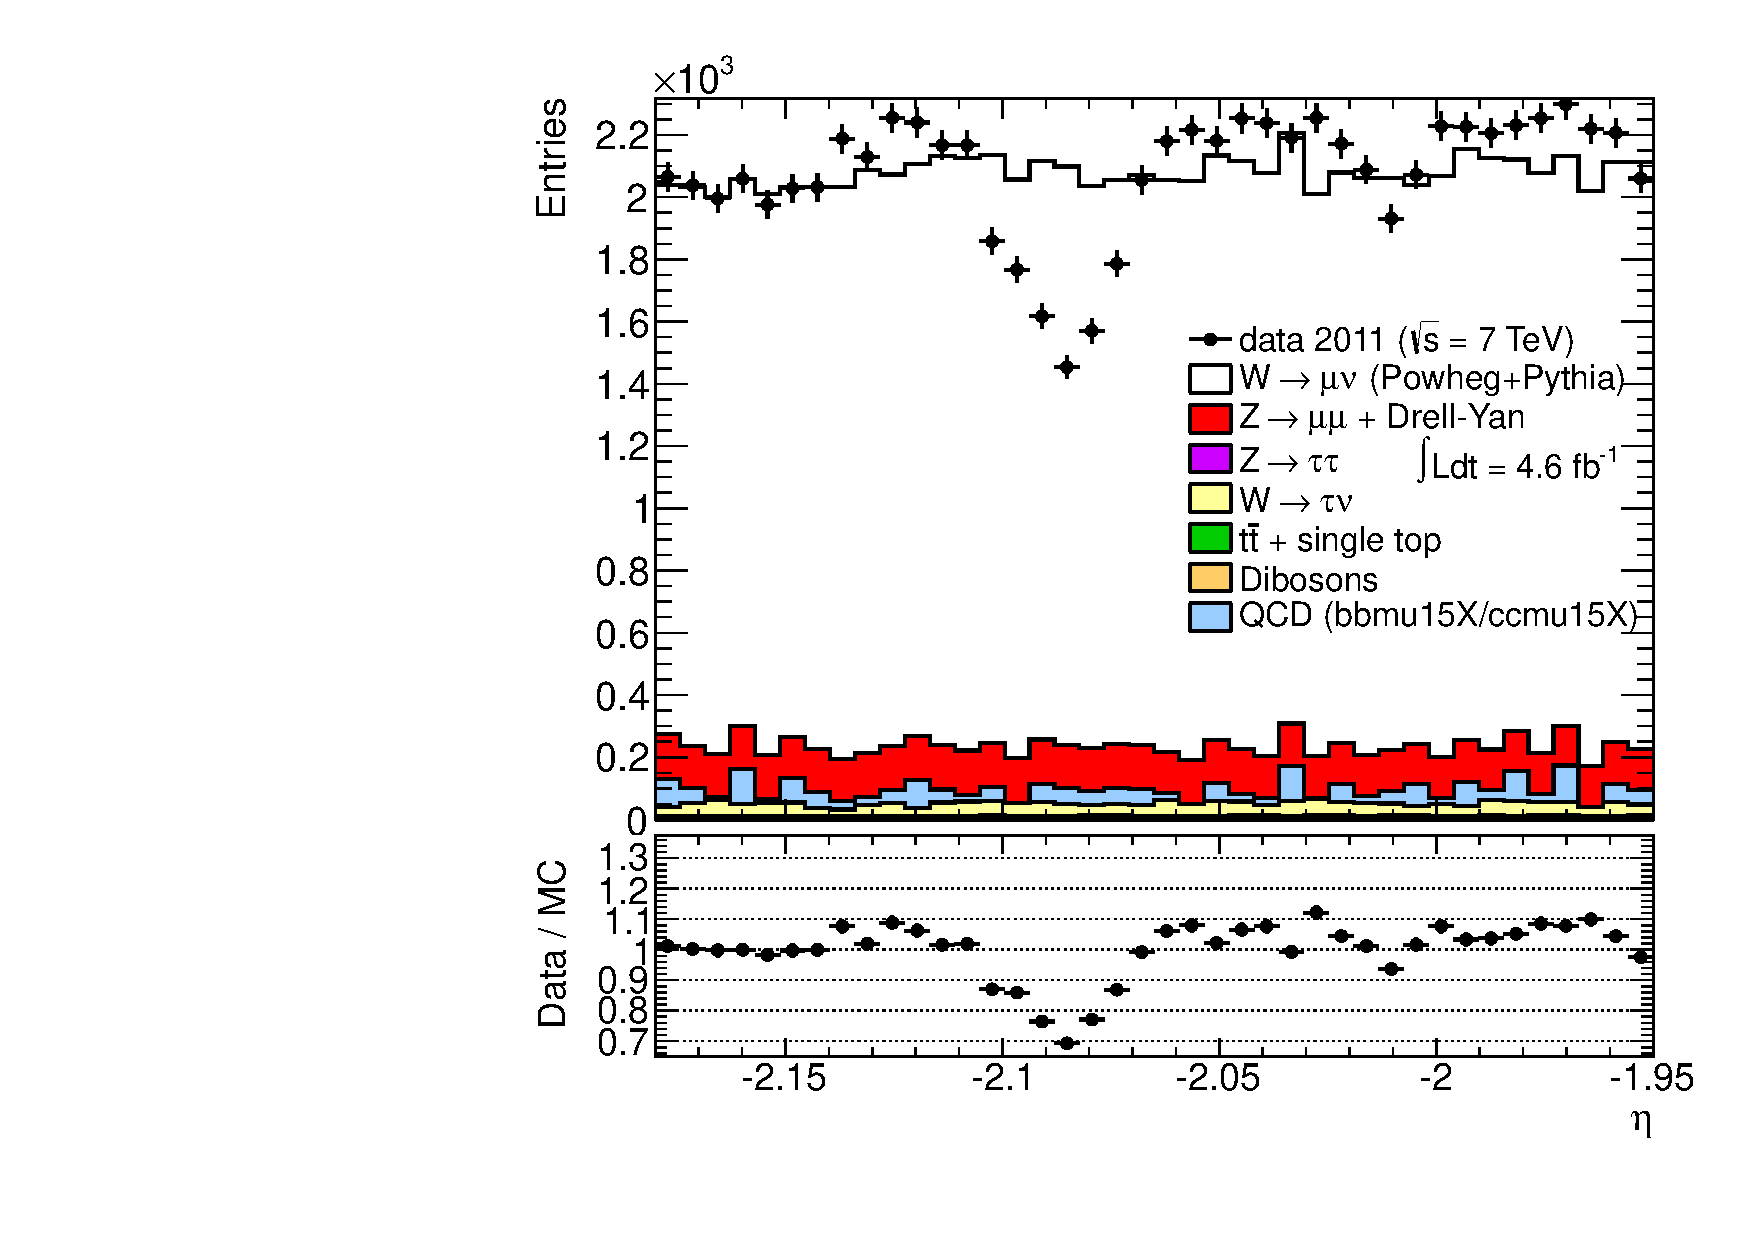
\includegraphics[width=0.66\textwidth]{dates/20130306/figures/both/WpLtoL_10_C_stack_l_eta_NEG} \\
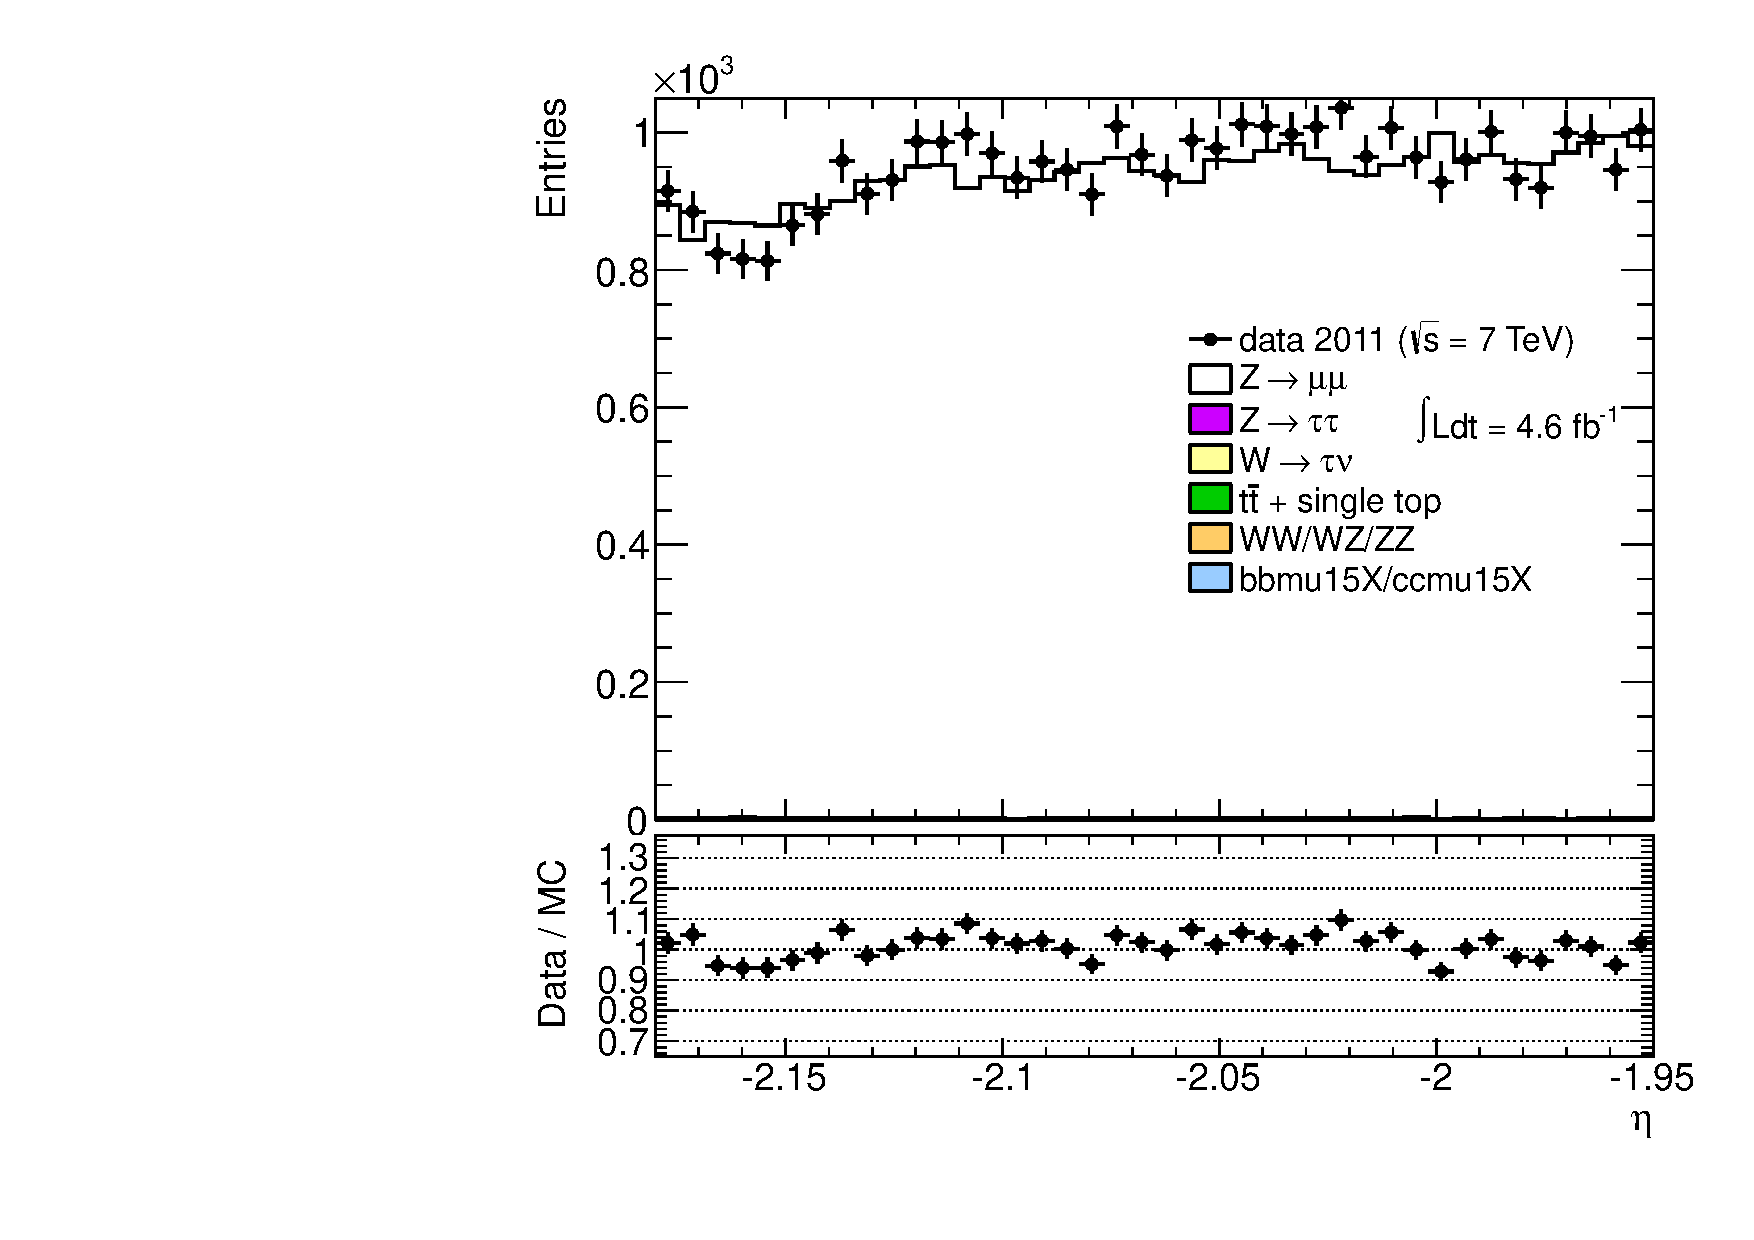
\includegraphics[width=0.66\textwidth]{dates/20130306/figures/both/Z_10_C_stack_lN_eta_ALL.pdf}
\column{.5\textwidth}
A-side $\mu^{-}$ (top: W; bottom: Z)
\centering
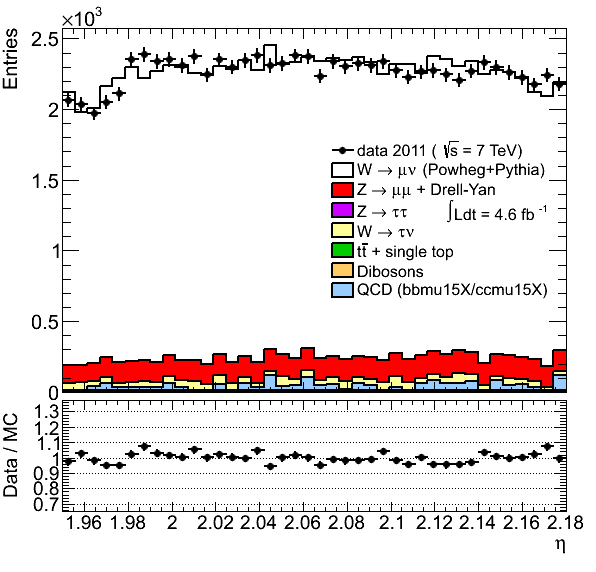
\includegraphics[width=0.66\textwidth]{dates/20130306/figures/both/WpLtoL_10_A_stack_l_eta_NEG} \\
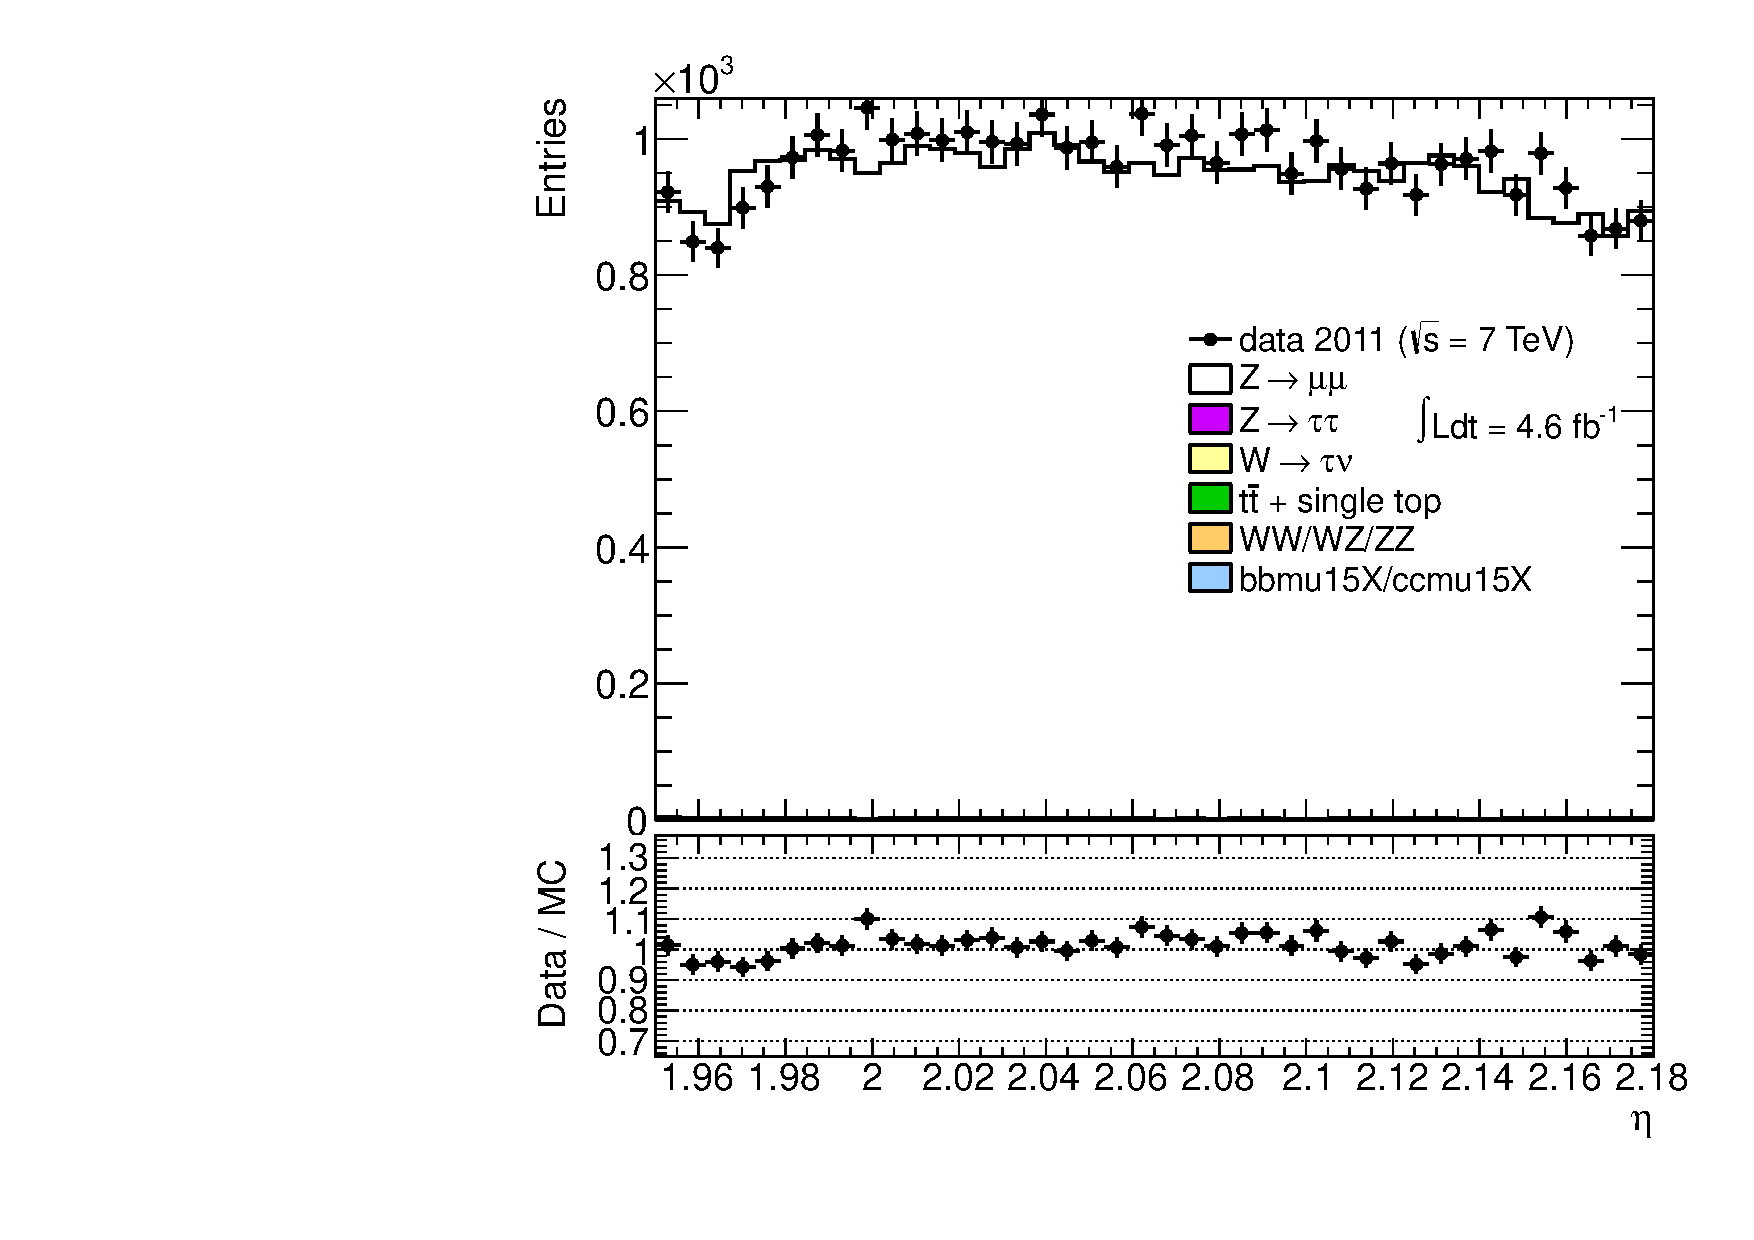
\includegraphics[width=0.66\textwidth]{dates/20130306/figures/both/Z_10_A_stack_lN_eta_ALL.pdf} 
\cole
}
\slide{ $\mu^{-}$: bin 10 ($1.95<\eta<2.18$), period M} {
\colb[T]
\column{.5\textwidth}
C-side $\mu^{-}$ (top: W; bottom: Z)
\centering
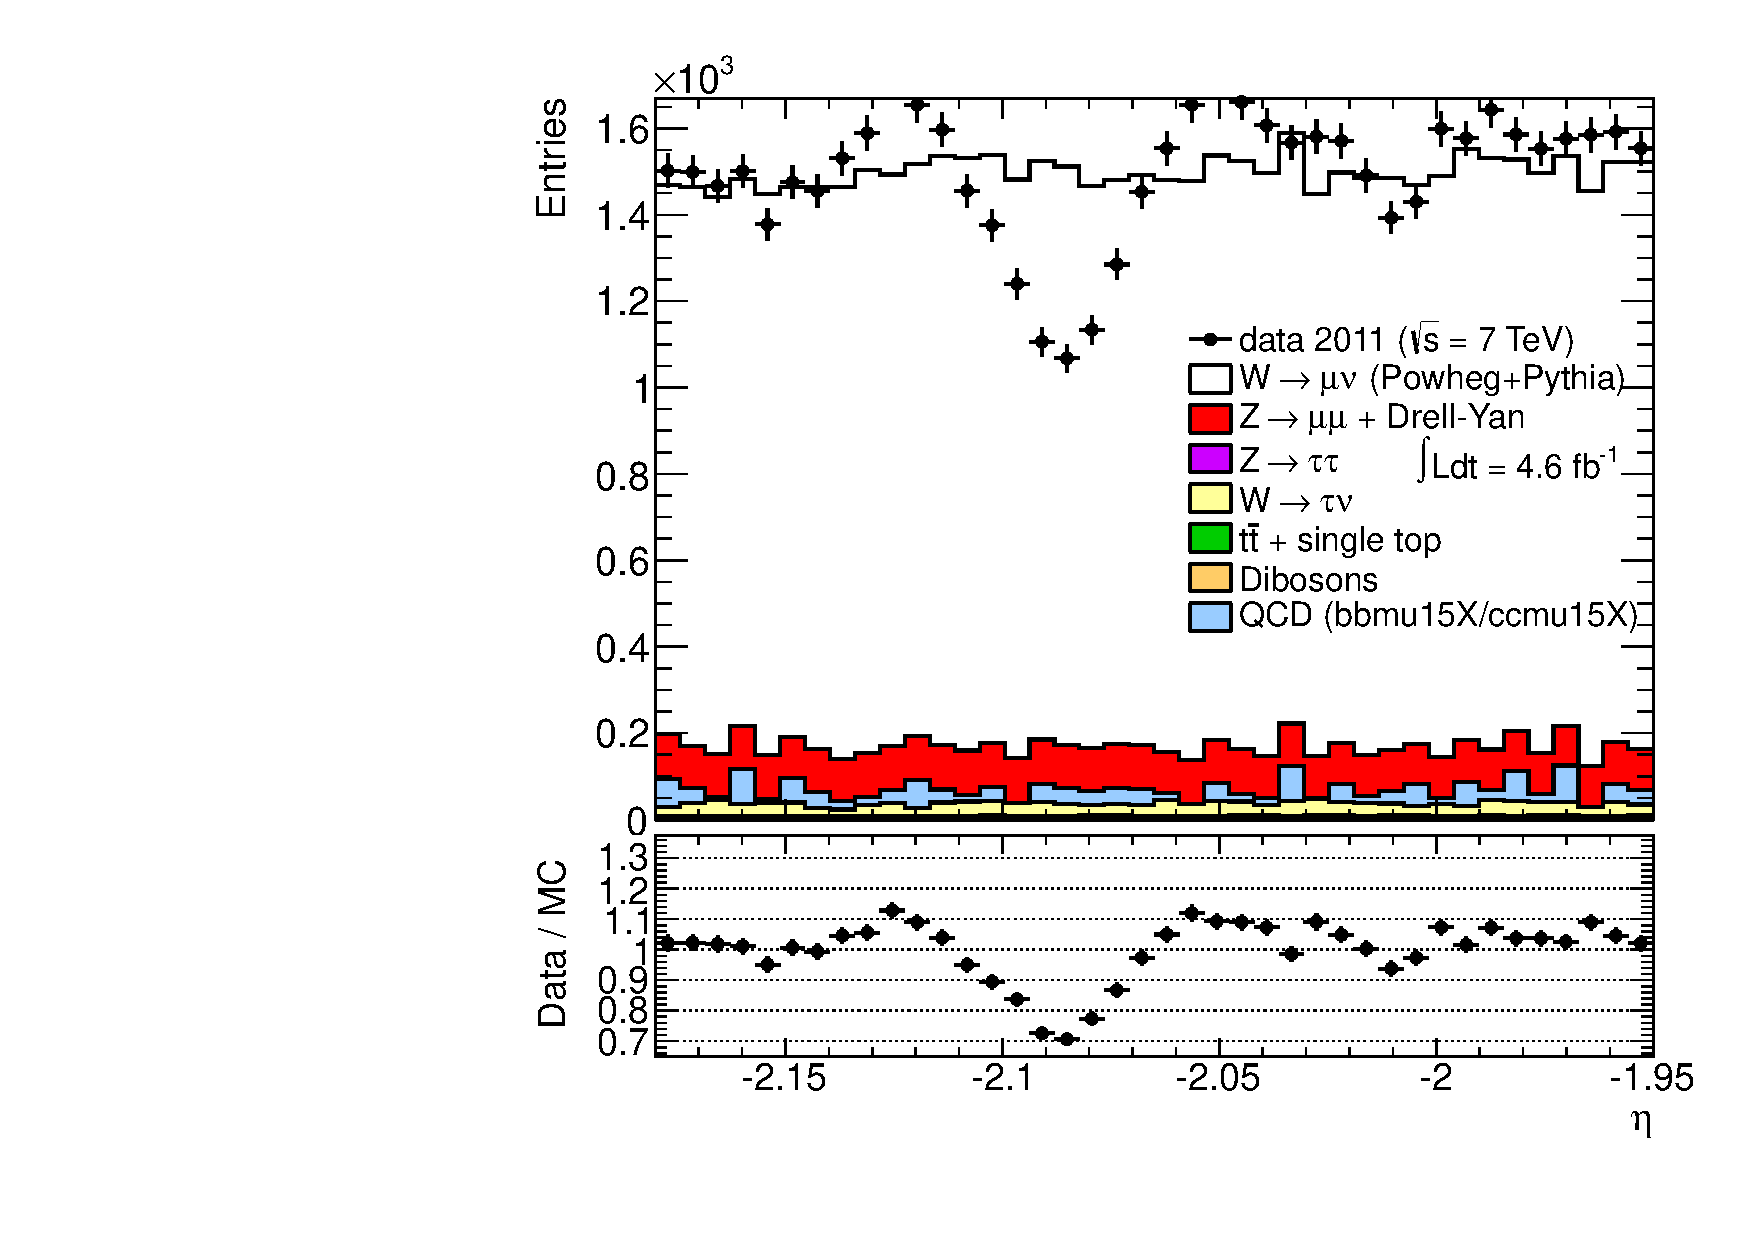
\includegraphics[width=0.66\textwidth]{dates/20130306/figures/both/WpMtoM_10_C_stack_l_eta_NEG} \\
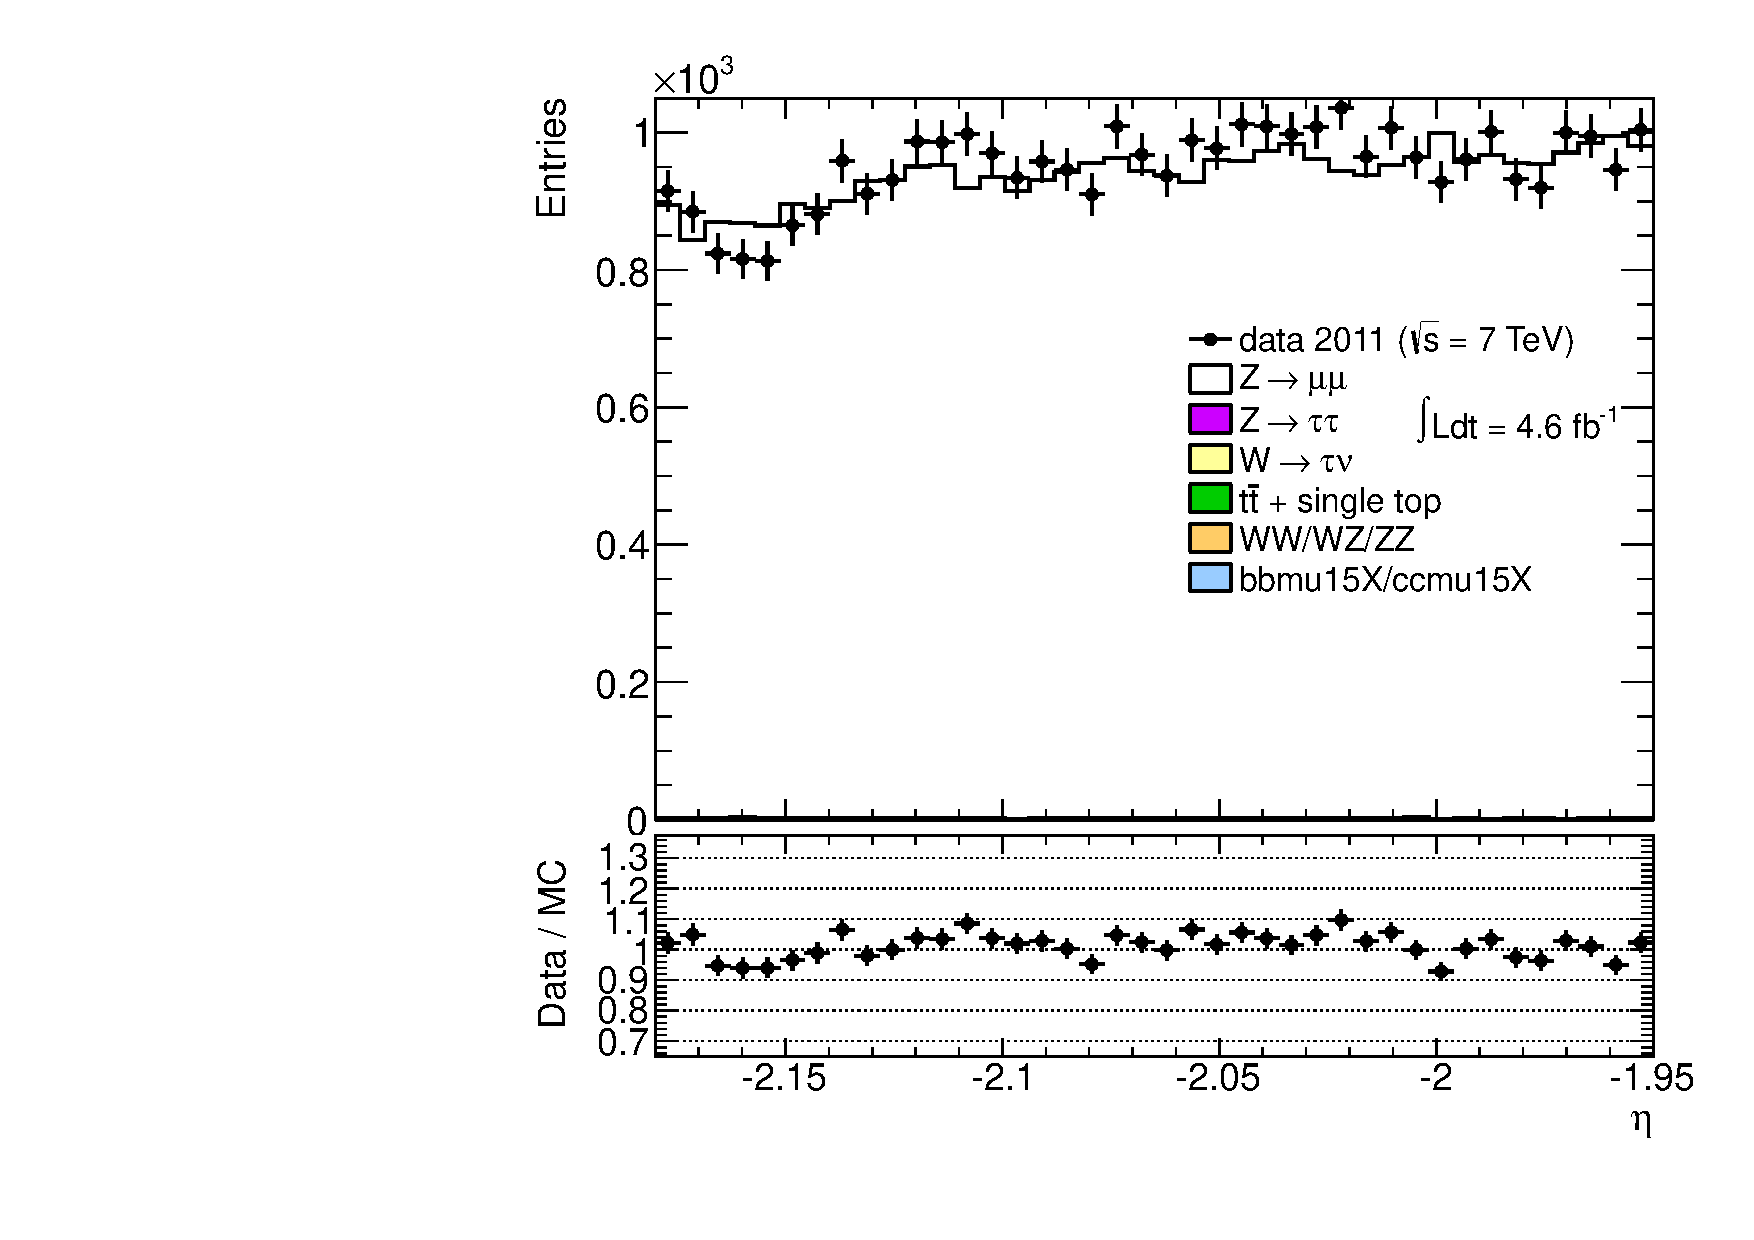
\includegraphics[width=0.66\textwidth]{dates/20130306/figures/both/Z_10_C_stack_lN_eta_ALL.pdf}
\column{.5\textwidth}
A-side $\mu^{-}$ (top: W; bottom: Z)
\centering
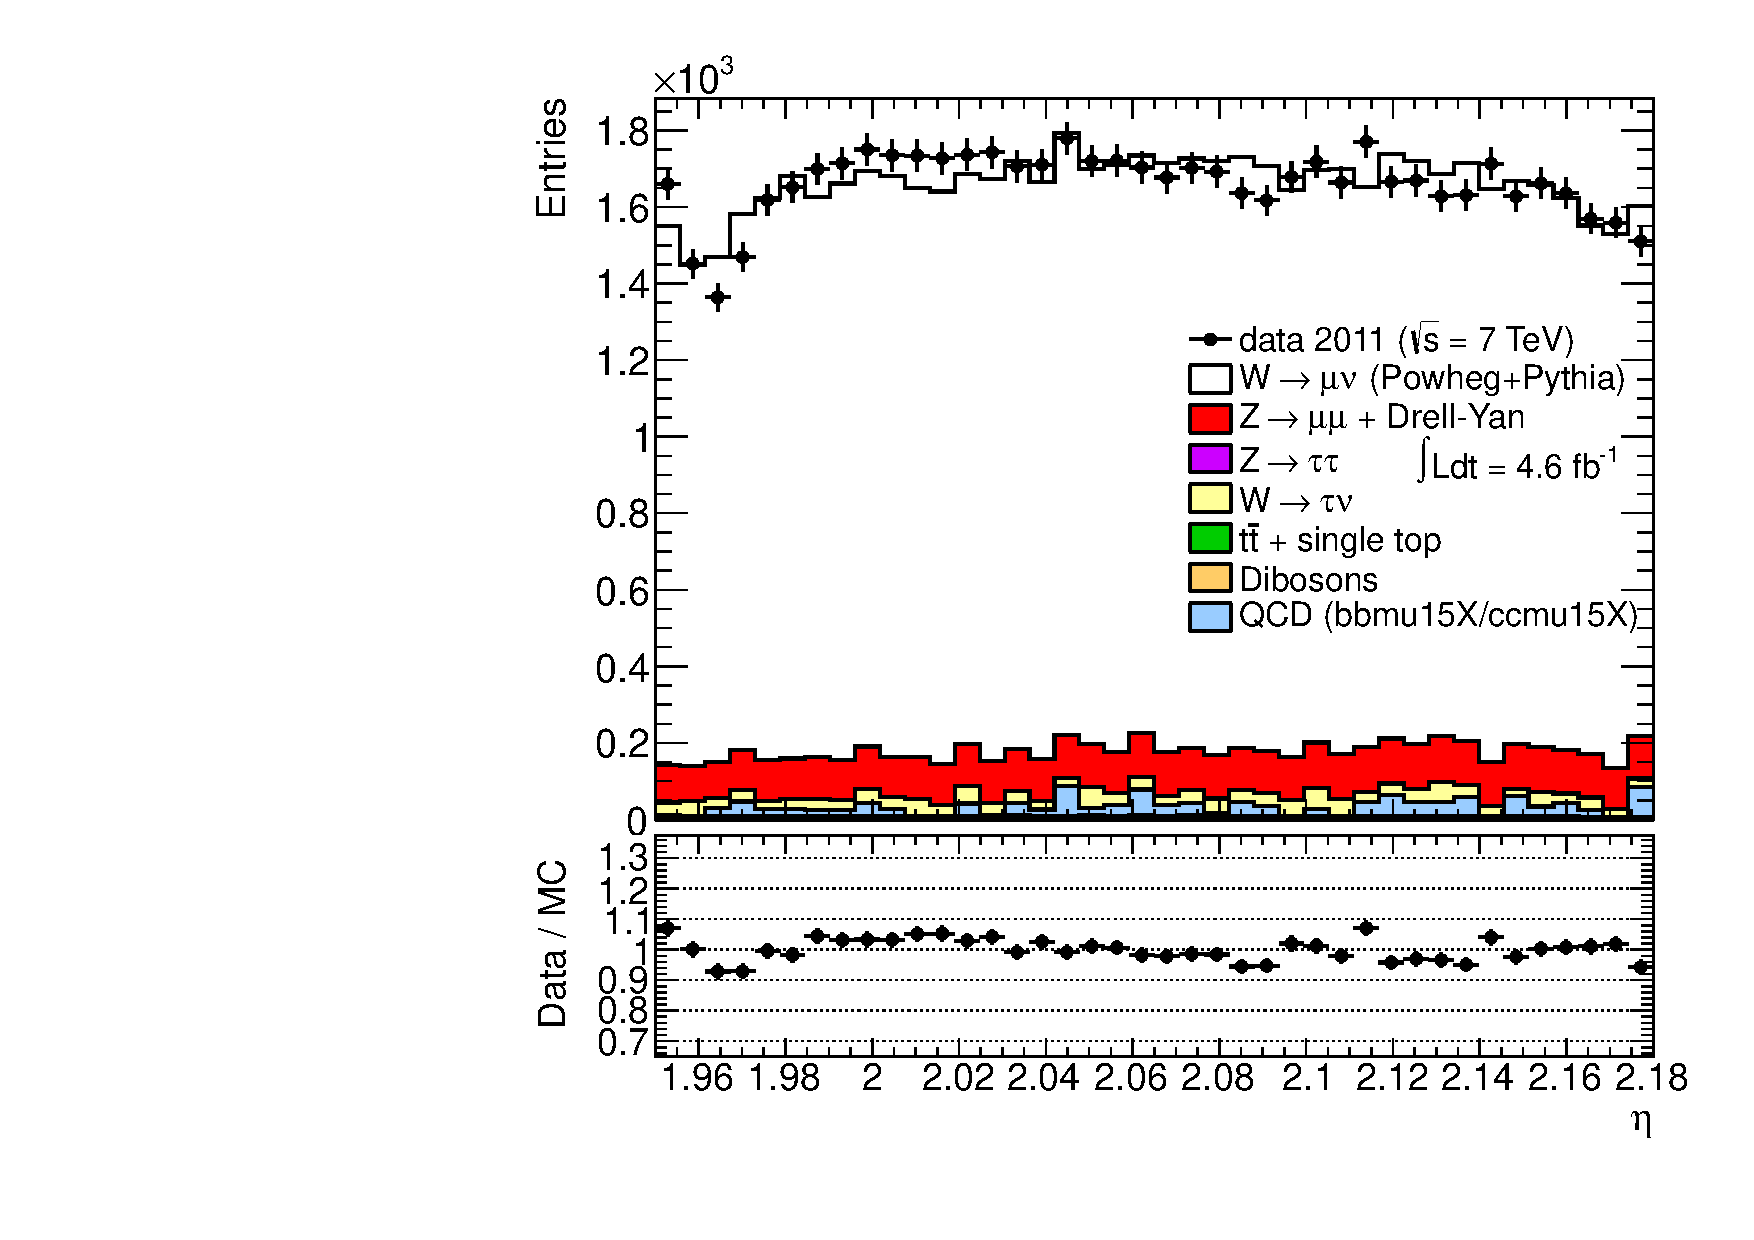
\includegraphics[width=0.66\textwidth]{dates/20130306/figures/both/WpMtoM_10_A_stack_l_eta_NEG} \\
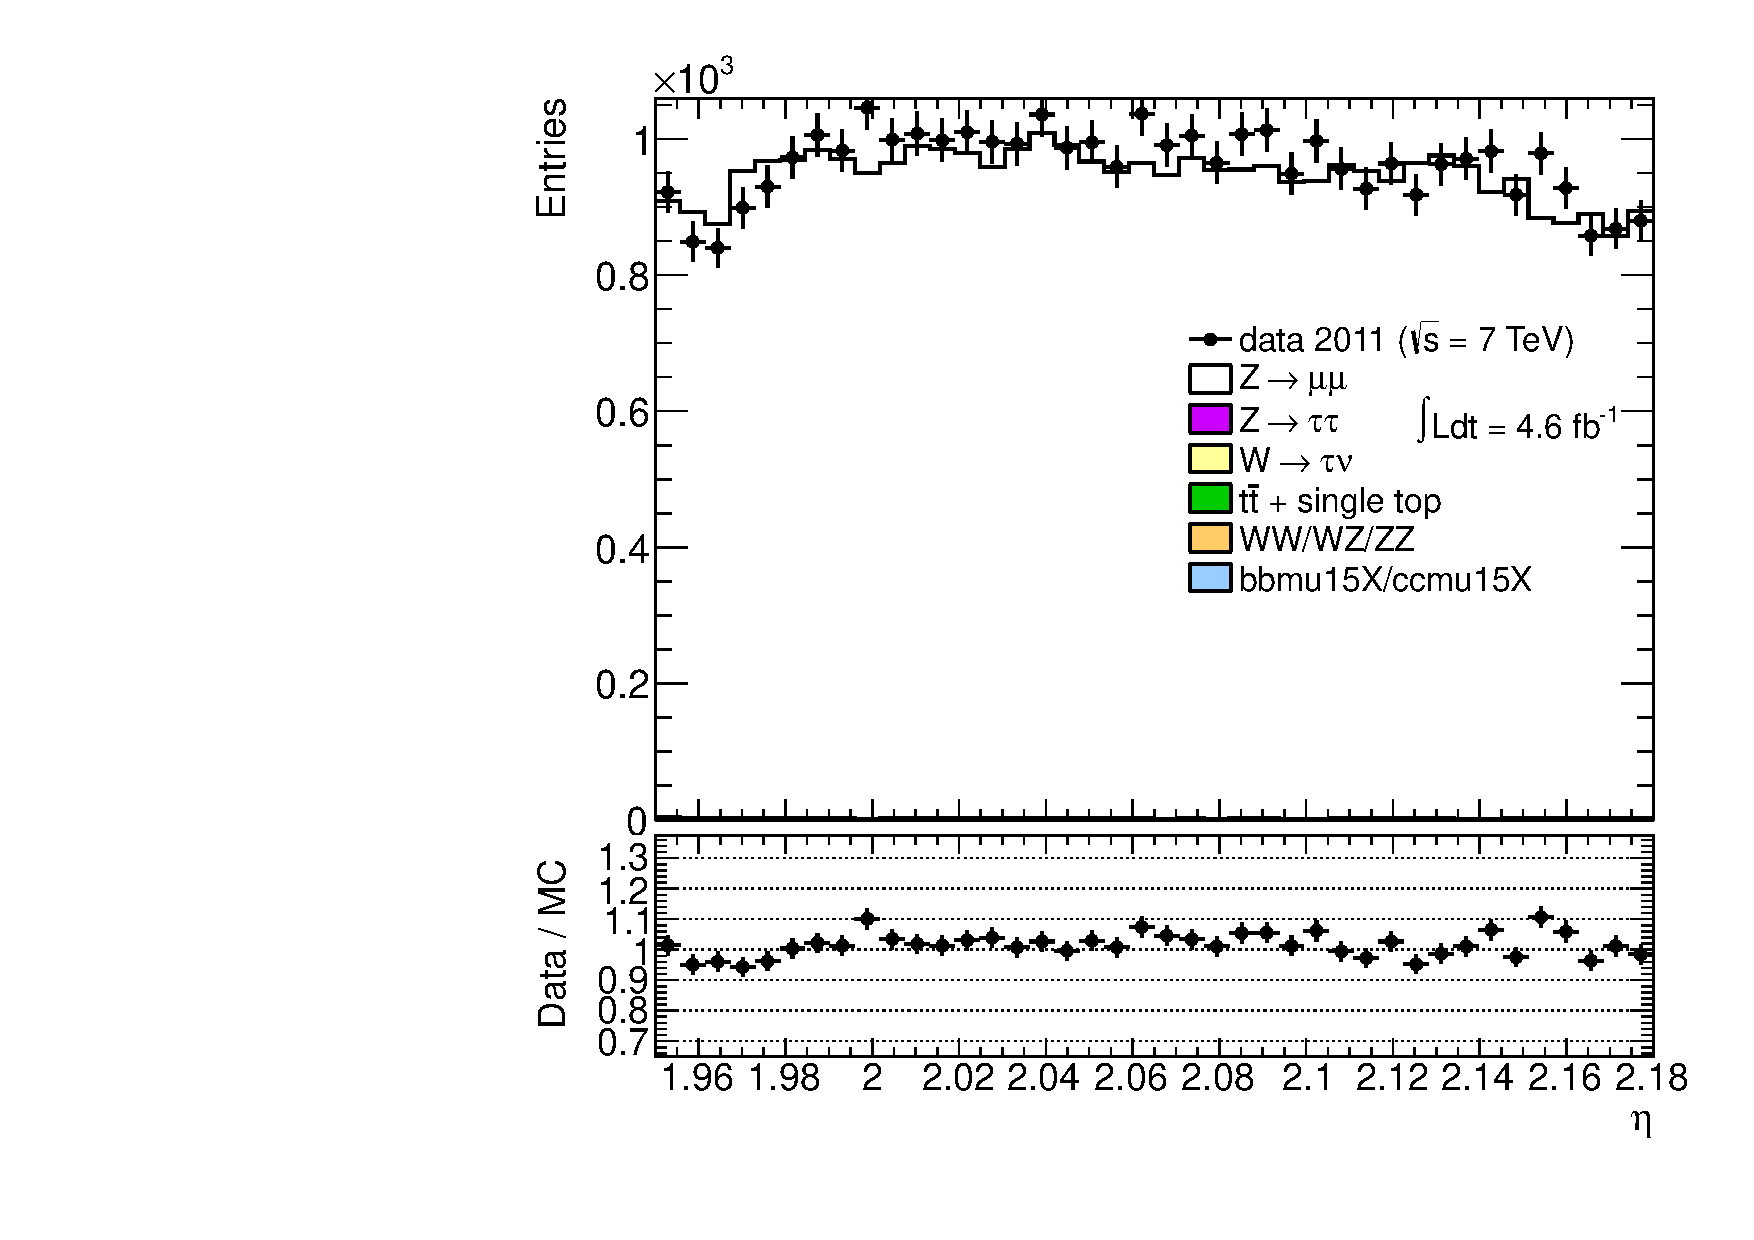
\includegraphics[width=0.66\textwidth]{dates/20130306/figures/both/Z_10_A_stack_lN_eta_ALL.pdf} 
\cole
}

% mu18mg vs mu18
\slide{ mu18MG vs mu18 trigger} {
 The dips appears in period I and stays for the rest of 2011 data taking. \\
 Recall that the dips (in W selection only) are seen with MG triggers. \\
 What about the muid trigger chains (mu18 and mu18medium)? \\
 In the plots below, both Ws and Zs were re-run with muid trigger chain. \\
 (caveat: still using MG-based trigger scale factors)
}

\slide{ $\mu^{-}$: bin 10 ($1.95<\eta<2.18$), mu18MG (nominal)} {
\colb[T]
\column{.5\textwidth}
C-side (top: W; bottom: Z)
\centering
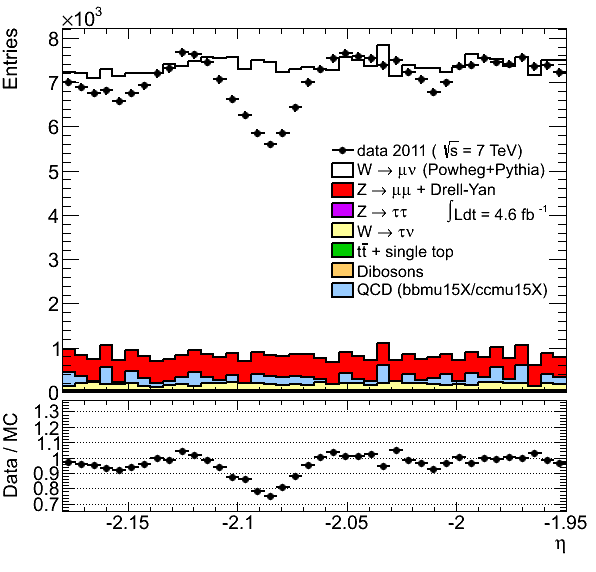
\includegraphics[width=0.66\textwidth]{dates/20130306/figures/mu18/WMU18_MG_10_C_stack_l_eta_NEG} \\
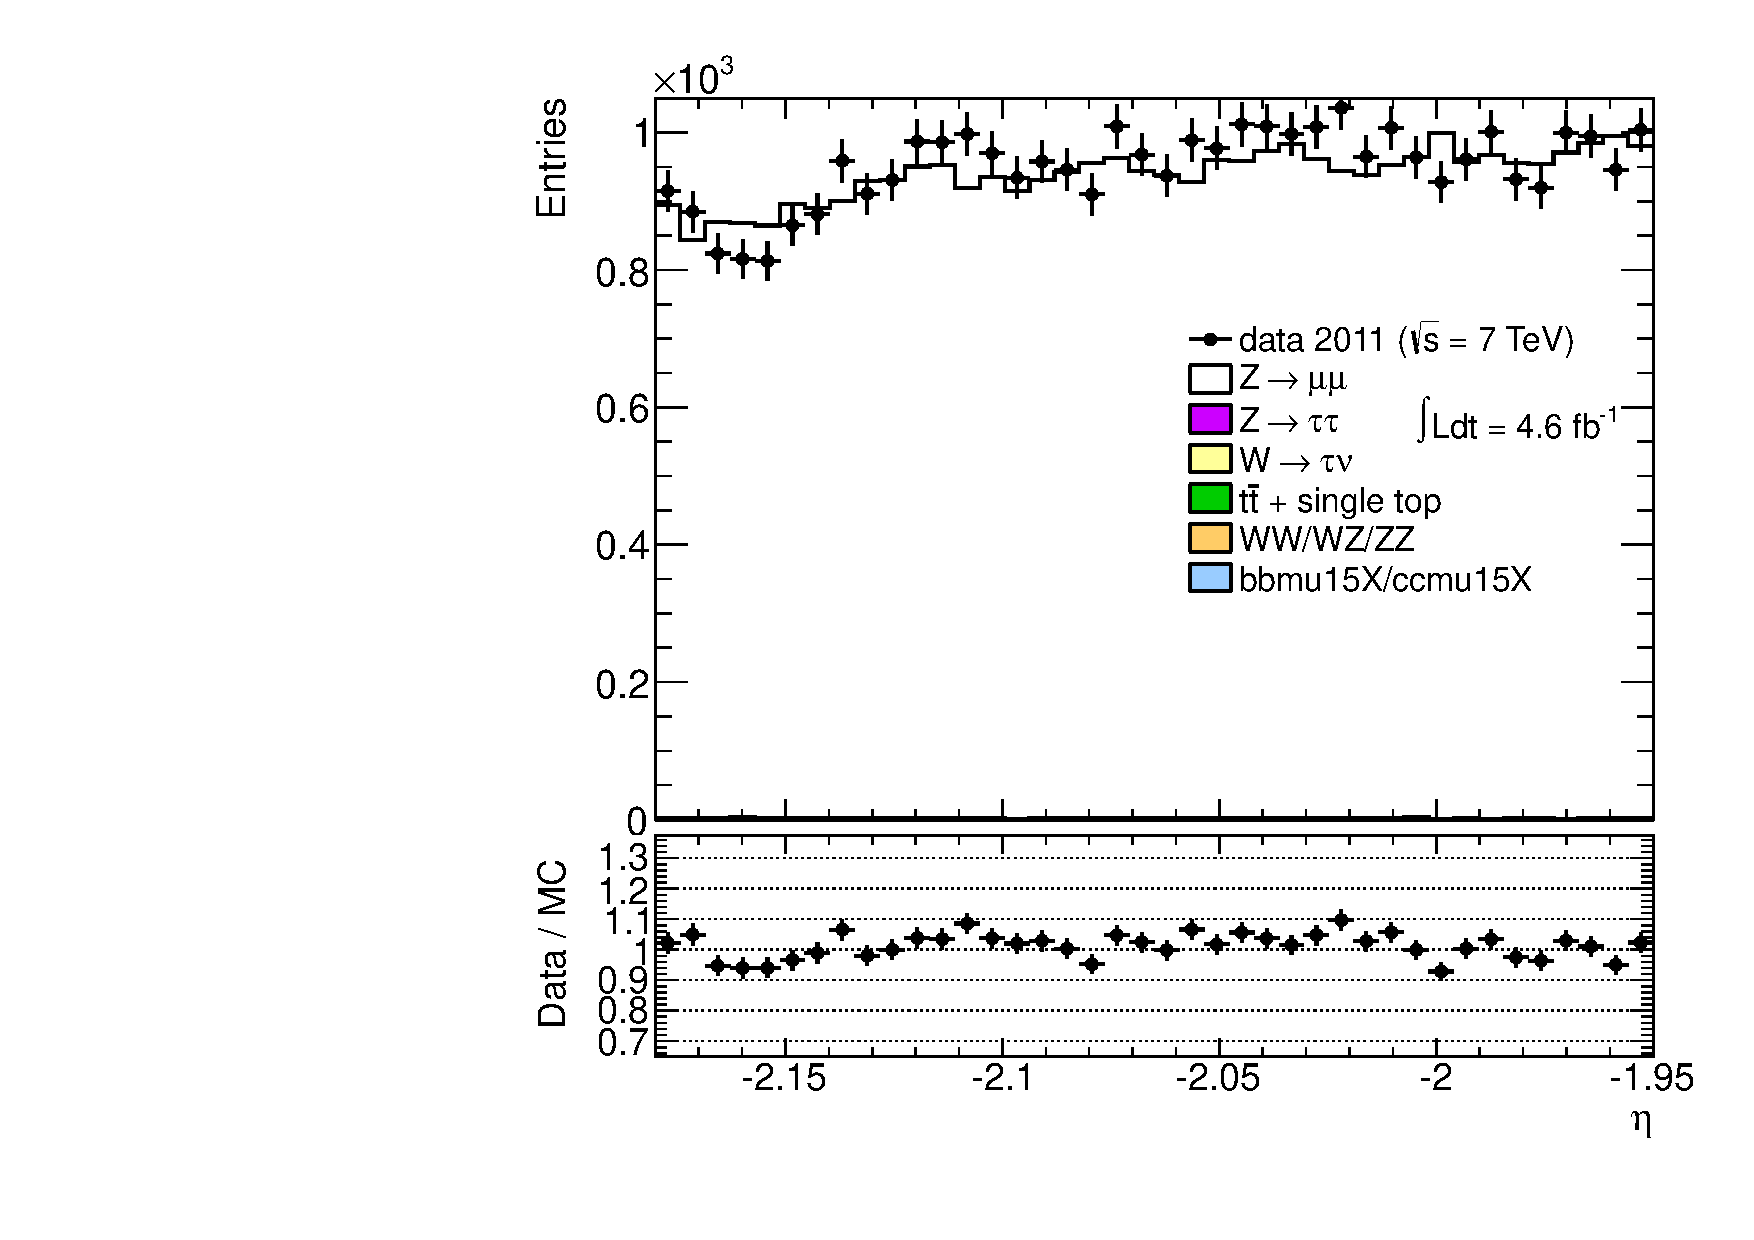
\includegraphics[width=0.66\textwidth]{dates/20130306/figures/mu18/ZMU18_MG_10_C_stack_lN_eta_ALL.pdf}
\column{.5\textwidth}
A-side (top: W; bottom: Z)
\centering
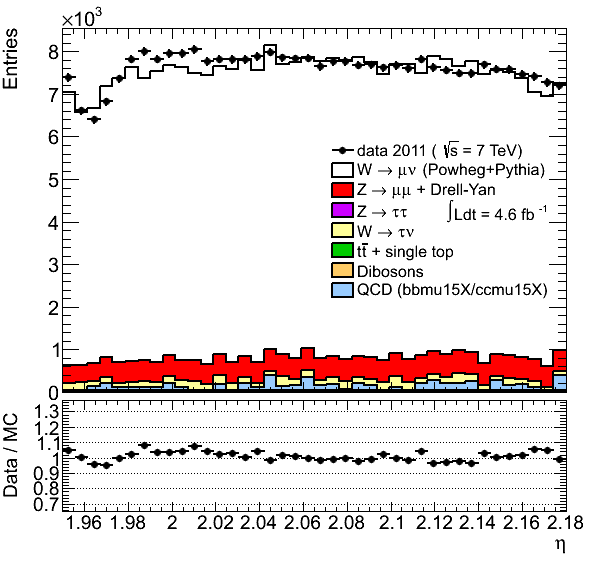
\includegraphics[width=0.66\textwidth]{dates/20130306/figures/mu18/WMU18_MG_10_A_stack_l_eta_NEG} \\
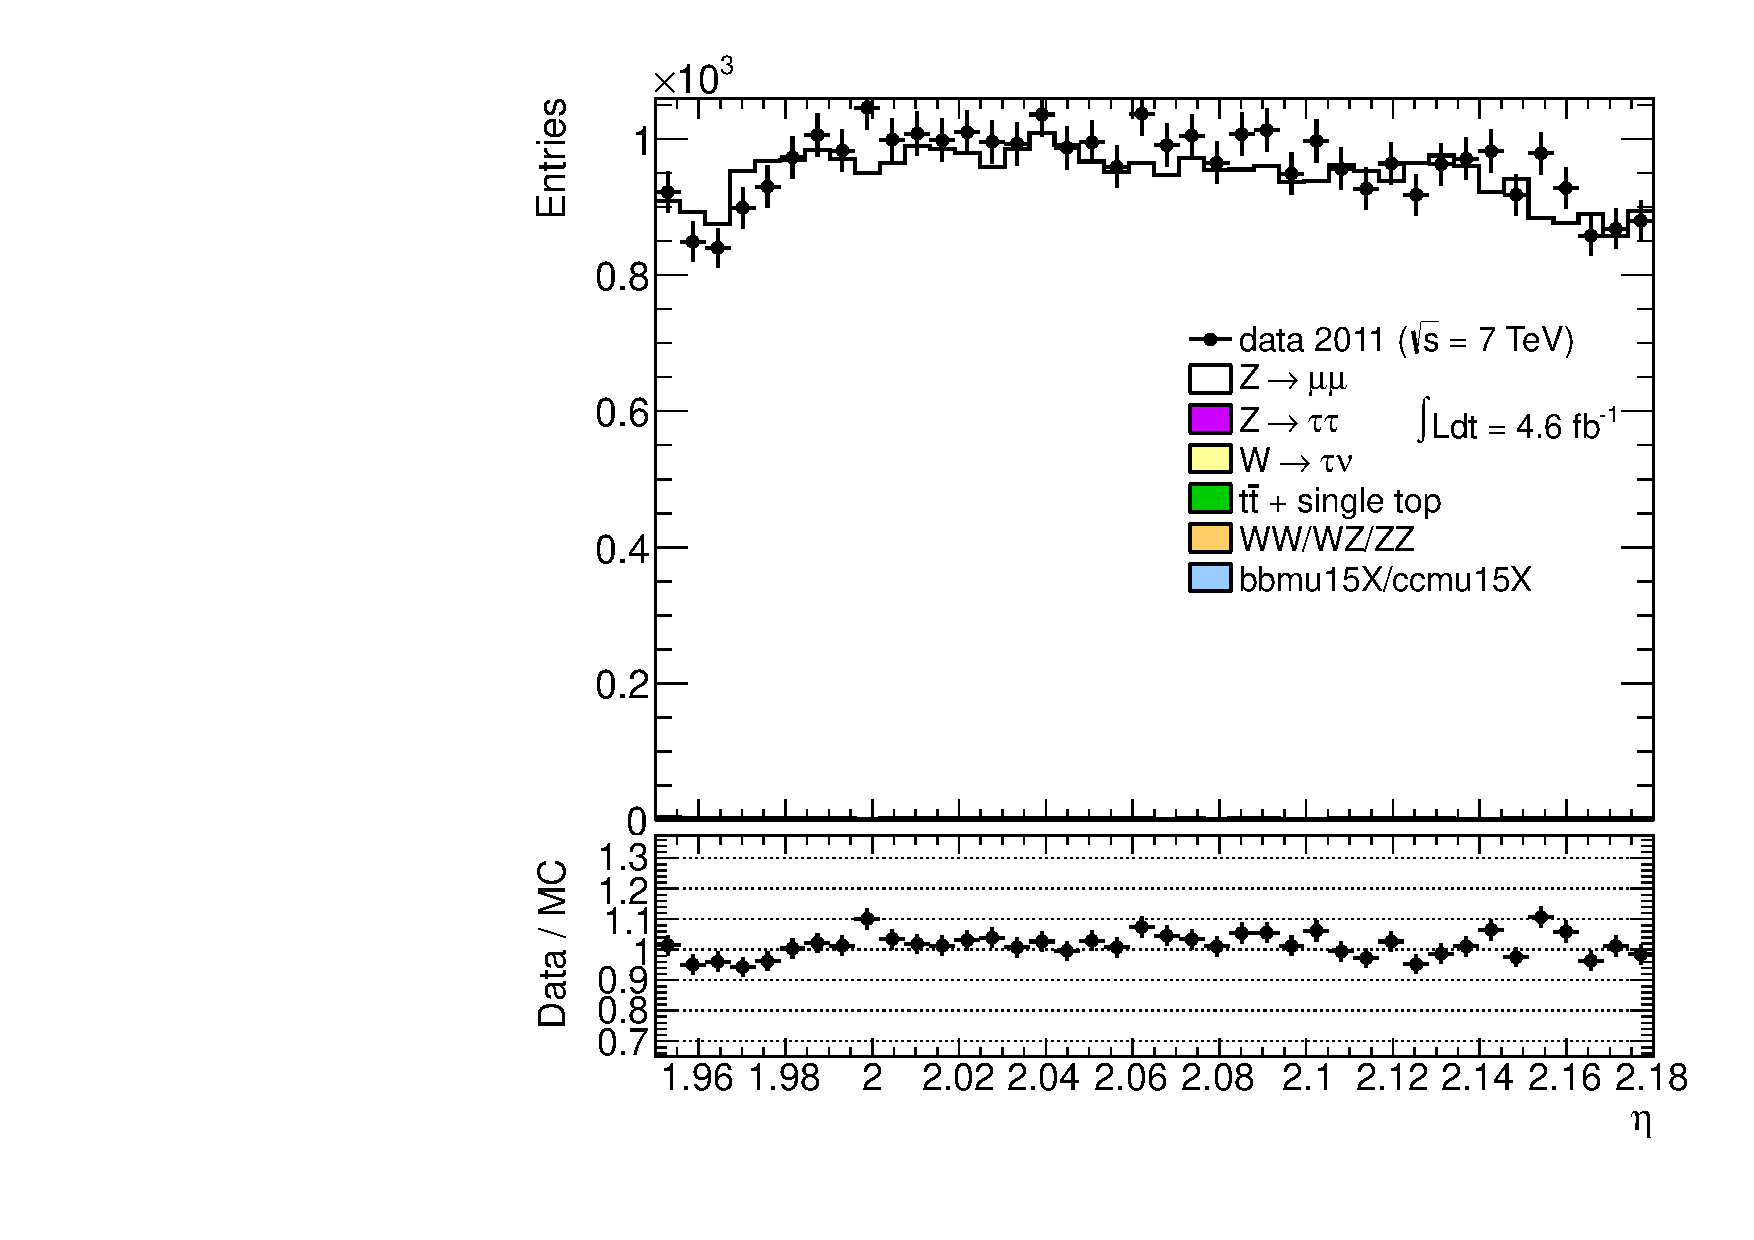
\includegraphics[width=0.66\textwidth]{dates/20130306/figures/mu18/ZMU18_MG_10_A_stack_lN_eta_ALL.pdf} 
\cole
}
\slide{ $\mu^{-}$: bin 10 ($1.95<\eta<2.18$), mu18 } {
\colb[T]
\column{.5\textwidth}
C-side (top: W; bottom: Z)
\centering
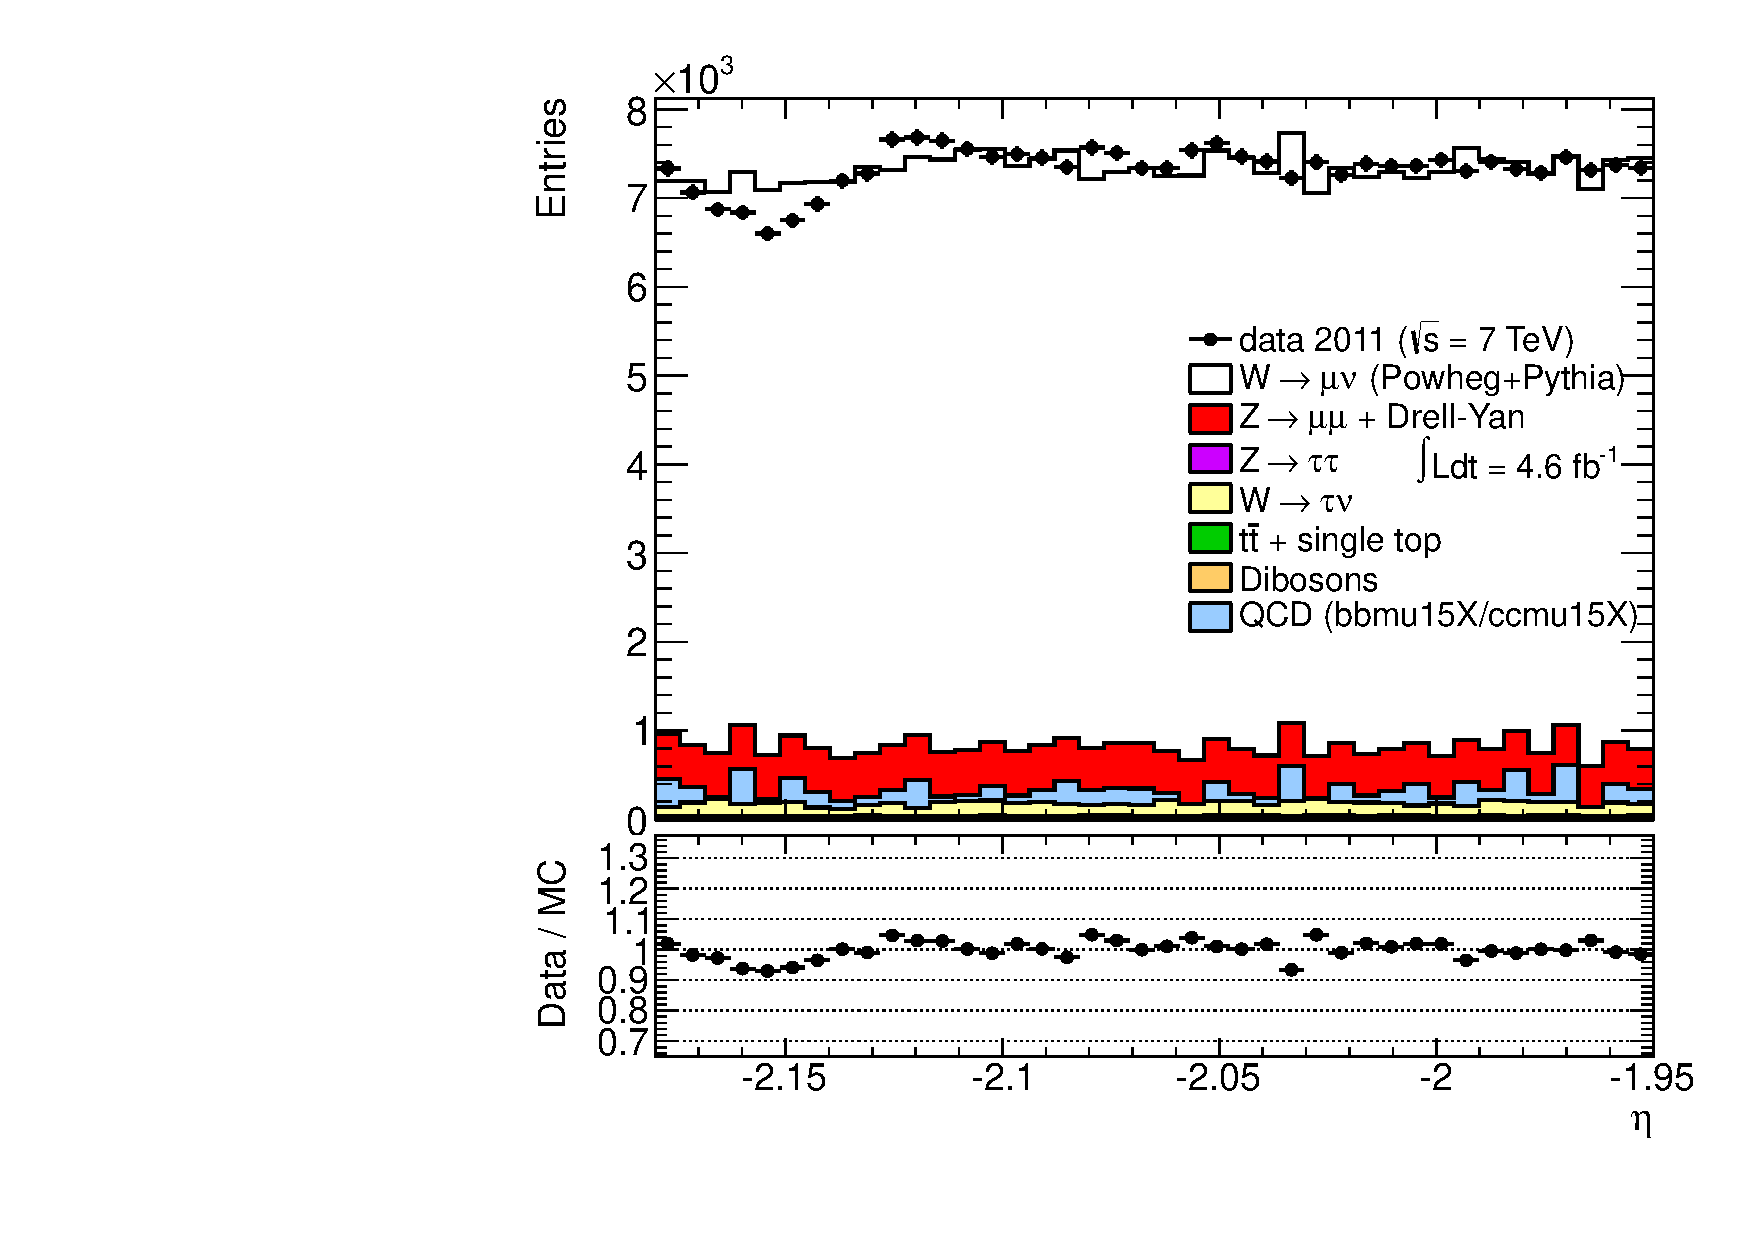
\includegraphics[width=0.66\textwidth]{dates/20130306/figures/mu18/WMU18_10_C_stack_l_eta_NEG} \\
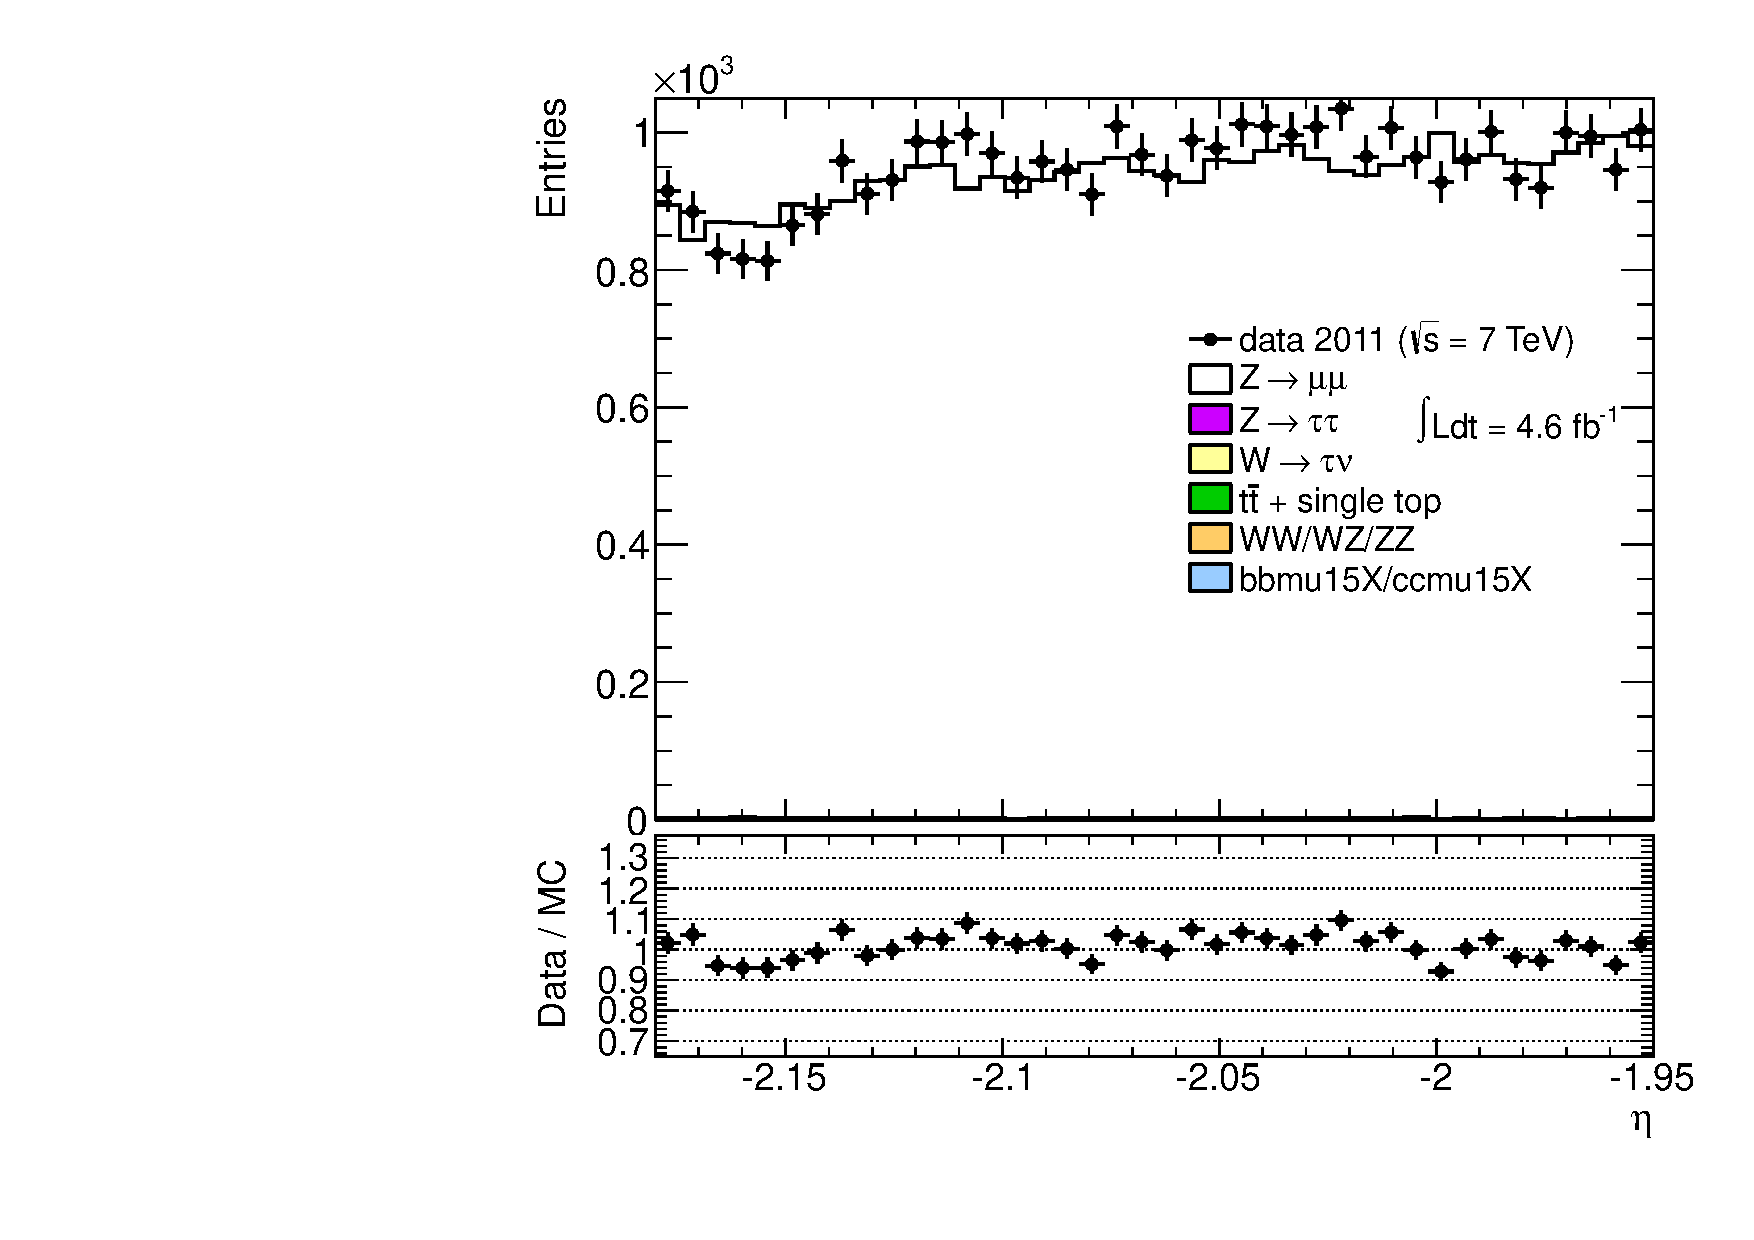
\includegraphics[width=0.66\textwidth]{dates/20130306/figures/mu18/ZMU18_10_C_stack_lN_eta_ALL.pdf}
\column{.5\textwidth}
A-side (top: W; bottom: Z)
\centering
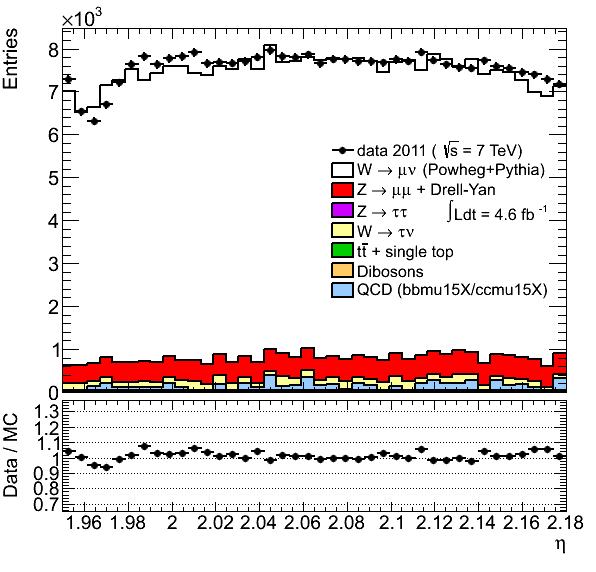
\includegraphics[width=0.66\textwidth]{dates/20130306/figures/mu18/WMU18_10_A_stack_l_eta_NEG} \\
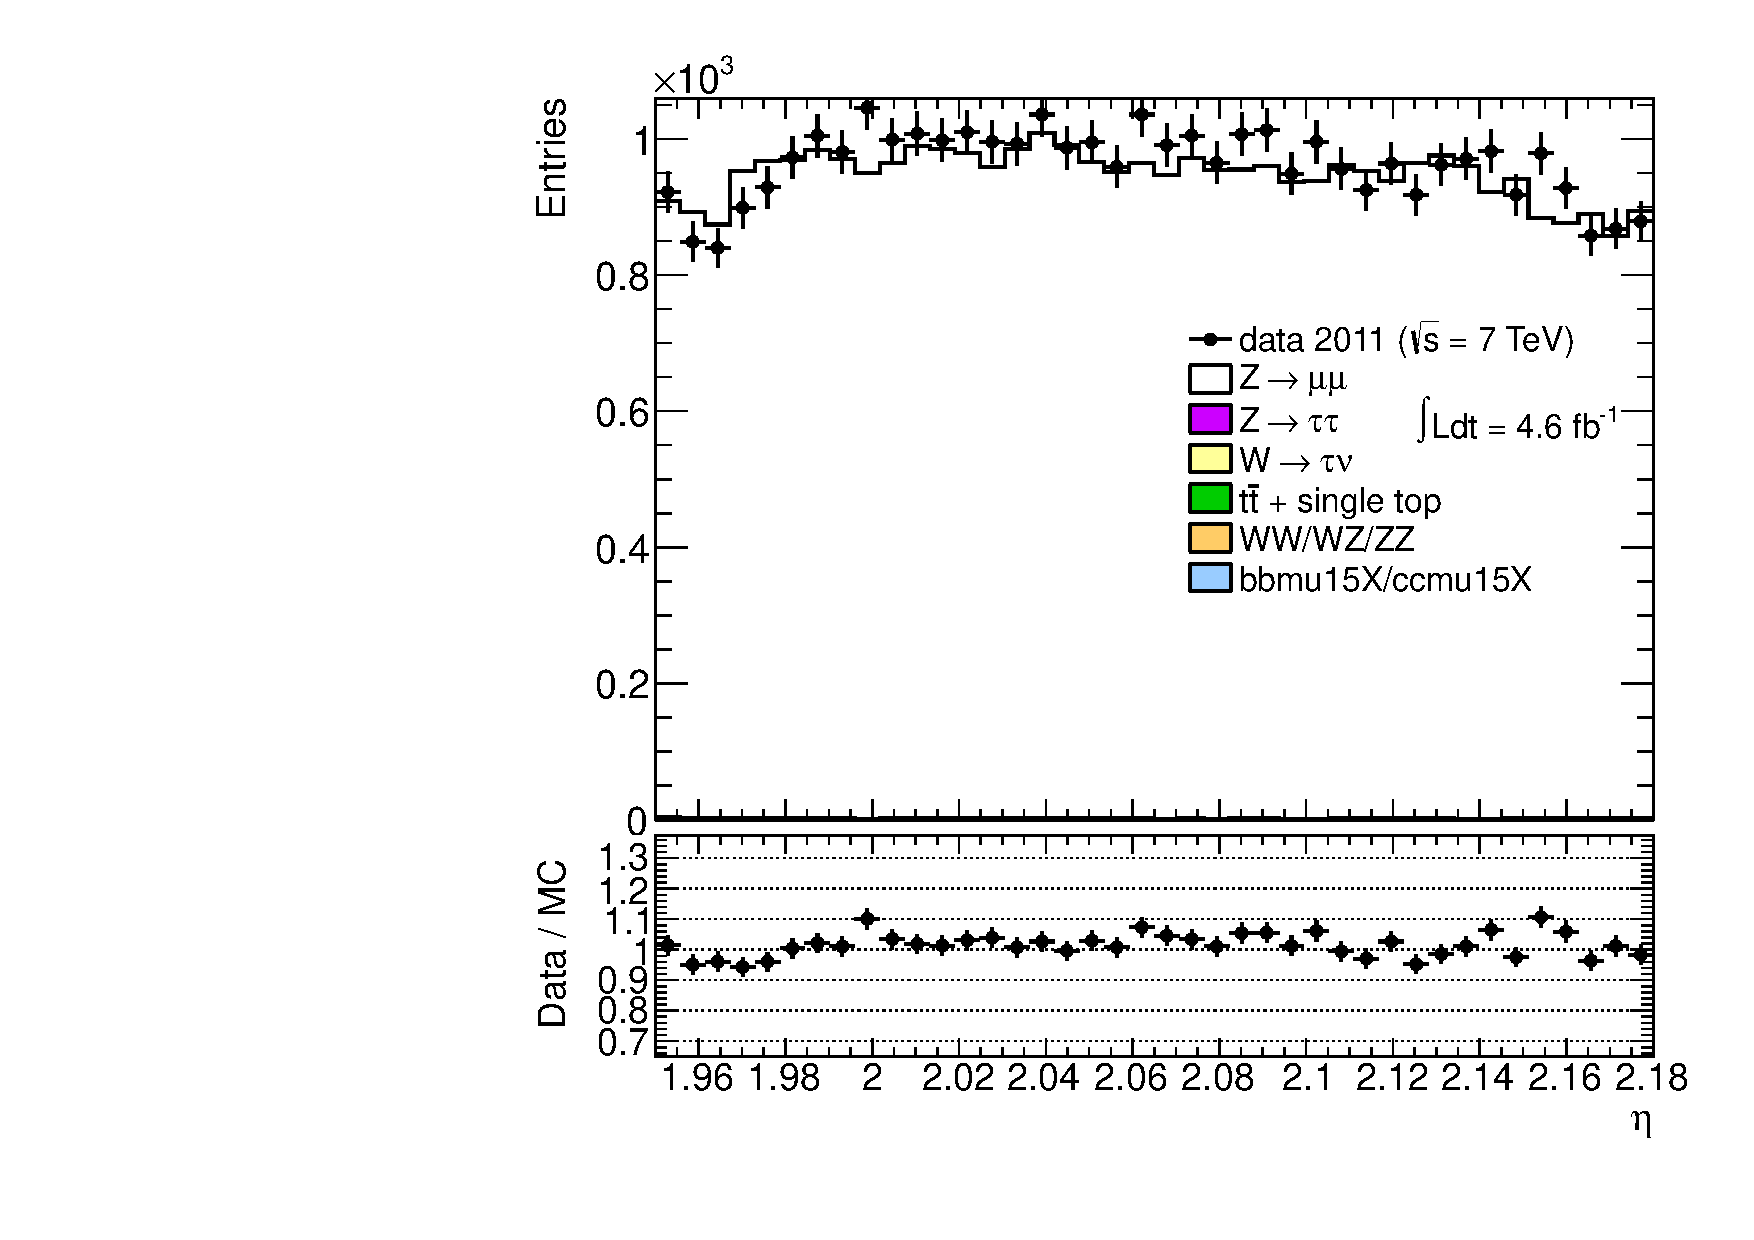
\includegraphics[width=0.66\textwidth]{dates/20130306/figures/mu18/ZMU18_10_A_stack_lN_eta_ALL.pdf} 
\cole
}

% mu18 vs mu18 MG - 2d plots
\slide{ mu18 vs mu18MG  } {
 Z events look the same with either trigger chain. \\
 But the W dip is NOT present when triggred by the muid trigger! \\
 To quantify this better, let's make 2D eta-phi plots for full W selection, where:
 \iteb
 \item mu18MG trigger succeeds, but mu18 fails
 \item mu18MG trigger fails, but mu18 succeeds
 \itee
}
% p.1
\slide{ mu18MG vs mu18: mu18MG succeeds  } {
\colb[T]
\column{.5\textwidth}
$\mu^+$: Period D
\centering
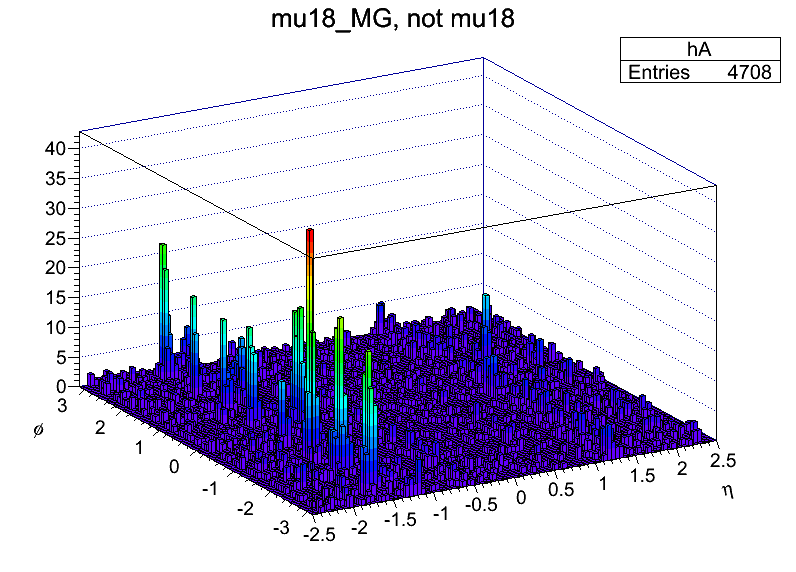
\includegraphics[width=0.95\textwidth]{dates/20130306/figures/mu18/dump_MG_dataD_w_POS.dat__MG_NOT_MUID.png}
\column{.5\textwidth}
$\mu^-$: Period D
\centering
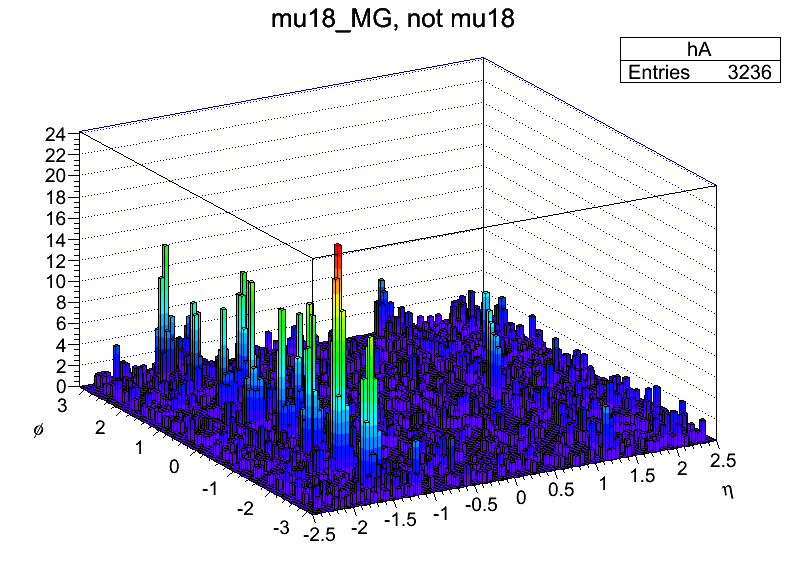
\includegraphics[width=0.95\textwidth]{dates/20130306/figures/mu18/dump_MG_dataD_w_NEG.dat__MG_NOT_MUID.png}
\cole
}
\slide{ mu18MG vs mu18: mu18MG succeeds  } {
\colb[T]
\column{.5\textwidth}
$\mu^+$: Period L
\centering
\includegraphics[width=0.95\textwidth]{dates/20130306/figures/mu18/dump_MG_dataL_w_POS.dat__MG_NOT_MUID.png}
\column{.5\textwidth}
$\mu^-$: Period L
\centering
\includegraphics[width=0.95\textwidth]{dates/20130306/figures/mu18/dump_MG_dataL_w_NEG.dat__MG_NOT_MUID.png}
\cole
}
% p.2
\slide{ mu18MG vs mu18: mu18 succeeds  } {
\colb[T]
\column{.5\textwidth}
$\mu^+$: Period D
\centering
\includegraphics[width=0.95\textwidth]{dates/20130306/figures/mu18/dump_MG_dataD_w_POS.dat__MUID_NOT_MG.png}
\column{.5\textwidth}
$\mu^-$: Period D
\centering
\includegraphics[width=0.95\textwidth]{dates/20130306/figures/mu18/dump_MG_dataD_w_NEG.dat__MUID_NOT_MG.png}
\cole
}
\slide{ mu18MG vs mu18: mu18MG succeeds  } {
\colb[T]
\column{.5\textwidth}
$\mu^+$: Period L
\centering
\includegraphics[width=0.95\textwidth]{dates/20130306/figures/mu18/dump_MG_dataL_w_POS.dat__MUID_NOT_MG.png}
\column{.5\textwidth}
$\mu^-$: Period L
\centering
\includegraphics[width=0.95\textwidth]{dates/20130306/figures/mu18/dump_MG_dataL_w_NEG.dat__MUID_NOT_MG.png}
\cole
}
\slide{ mu18 vs mu18MG  } {
  Conclusions: \\
  Remember that these plots do not rely on trigger matching - we simply use W selection with 1 muon, which HAD to trigger.
  We see that \red{something happened to the MG trigger on the C-side in later data periods}. The mu18 trigger is not affected. \\
  Coupled with the fact that the trigger matching is not working correctly in Z events with MG chains, this C-side MG inefficiency biases the trigger scale factors and introduces A/C asymmetry in the W analysis.
}

\slide{ Conclusions } {
 \iteb
 \item A/C disagreements in a particular bin are associated with a funny $\eta$ dip
 \item Made attempts to introduce the dip in Z events, or remove in W events
 \iteb
 \item All kinematic and quality cuts have no effect
 \item Dips in W are \red{absent before period I}, but present thereafter
 \iteb
 \item Problem doesn't quite align with shift from mu18MG to mu18MGmedium, which happened \red{in the end of period I}.
 \item However, it aligns with the \red{technical stop}, which happened between period H and I.
 \itee
 \item The dips disappear whenever there is a second muon in the event (even if the probe is asked to match trigger!)
 \iteb
 \item At least in 10th $\eta$ bin, the dip re-appears in Z events if the other muon (tag) is explicitly required to \red{fail} trigger.
 \itee
 \item muid trigger chains (mu18 and mu18medium) to not seem to have the same C-side problems seen in MG chains.
 \itee
 \itee
}


%%%%%%% Back-up slides %%%%%%%%%%
\appendix
\newcounter{finalframe}
\setcounter{finalframe}{\value{framenumber}}

\slide{}
{

\centering
\Huge Back-up slides
}
